\documentclass[11pt]{article}
\usepackage[a4paper,margin=23mm]{geometry}
\usepackage{fontspec,xeCJK}
\setmainfont{DejaVu Serif}
\setmonofont{DejaVu Sans Mono}[Scale=0.85]
\setCJKmainfont[AutoFakeBold=2,AutoFakeSlant=0.15]{Droid Sans Fallback}
\setCJKmonofont{Droid Sans Fallback}
\xeCJKDeclareCharClass{Default}{"201C,"201D}
\setlength{\emergencystretch}{2em}
\usepackage{amsmath,amssymb,bm,booktabs,longtable,array}
\usepackage{xcolor,graphicx,tikz}
\usetikzlibrary{arrows.meta,positioning,decorations.pathreplacing}
\usepackage[colorlinks=true,linkcolor=blue!55!black,urlcolor=blue!55!black]{hyperref}
\renewcommand{\contentsname}{目录}
\renewcommand{\abstractname}{摘要}
\renewcommand{\refname}{参考资料与代码依据}
\newcommand{\Tr}{\operatorname{Tr}}
\newcommand{\str}{\operatorname{str}}
\newcommand{\Pf}{\operatorname{Pf}}
\newcommand{\id}{\mathrm{id}}
\newcommand{\tS}{\widetilde S}
\newcommand{\code}[1]{\texttt{\small #1}}
\newcommand{\status}[1]{\par\smallskip\noindent\textbf{状态：#1。}\ }
\newcommand{\eps}{\varepsilon}
\title{严格 $D=2$ fermionic PEPS 与三分 Rényi 多副本环境\\
\large 局域张量、交换符号、six-$R$ 接缝及验证方案}
\author{研究设计 note}
\date{2026 年 9 月 9 日初稿；9 月 18 日更新双边求解与 bare/direct 数据}
\begin{document}
\maketitle
\begin{abstract}
目标是把手写 \code{fPEPS\_renyi\_2.pdf} 中的严格 Gaussian fPEPS 接到目前的
boundary VUMPS、LMPS 与 six-$R$ 计算上，并与 Gaussian 目录的三分多重熵比较。
本文给出局域 $D=2$ 张量的全部非零系数，固定占据数与 leg 顺序，区分
费米子重排的 graded swap 和观测量定义中的普通 replica permutation，
说明单副本双层吸收的符号为何不能直接替代多副本接缝的符号。
建议先建立有限网络的显式 swap 基准，再验证带符号的两周期分解，最后接入 six-$R$。
特别保留中心闭合、远端 cap、spin structure 和截断后 parity string 的信息。

局域 CAR 展开、384 个置换/奇偶组合，以及四模 Gaussian 占据数基准已做小规模数值核对；
后续已实现带完整宇称求和的 LMPS/six-$R$ 收缩，并完成有限网络独立符号检查。
2026 年 9 月 17 日将主路线纠正为两列／三列固定点的 bare/direct，
$w=1,\chi=4$ 的固定网络长度和相位检查通过，但重构一致性与物理精度尚未认证。
本文保留设计阶段的推导与验证要求，新增实现状态不构成无限 $\chi$ 正确性证明。
\end{abstract}
\tableofcontents
\newpage

\section{结论和研究对象}

\textbf{严格的 fPEPS 可以直接构造；主要难点在 environment 的符号约定和多副本闭合。}
这里的符号是反对易代数的确定性符号，不是要用 Monte Carlo 平均消除的随机权重问题。
应把它做成可验证的张量操作规则，而不是在最终标量上补一个经验负号。

建议采用以下顺序：
\begin{enumerate}
\item 固定 $Q$、有向虚键和物理 Fock 顺序，生成精确局域 $A$。
\item 在有限小网络上，从原始 ket/bra 和显式 swap 门计算
      $Z_1,Z_{2A},Z_{2B},Z_{2C},Z_4$，与占据数和 Gaussian 方法逐项比较。
\item 从同一套线序规则导出单副本双层、seam transfer、远端 cap 和中心闭合；
      所有截断保留 parity 与有向融合信息。
\item 验证四副本接缝能否在明确的带符号基变换下分成两个两周期。
      通过后才复用 six-$R$；否则先用完整四副本接缝或扩展 parity 通道。
\end{enumerate}

这里“严格”指局域张量以有限 $D$ 精确表示指定状态。
\textbf{有限 $\chi$ 的 VUMPS/LMPS 环境仍是近似。}
RK--Ising 是严格 $D=2$ 态；当前 TFIM 路线是 AD/CTMRG 优化有限 $D$ 张量，
再对已保存的态求 VUMPS 环境。fPEPS 的新计算应像 RK benchmark 一样固定 $A$，
把 $D$ 误差与 $\chi$ 误差分开，不能将 TFIM 的优化收敛逻辑直接照搬。

已有资料中的 \code{note\_fpeps\_en} 实际讨论的是 \emph{finite} RK--Ising PEPS，
不是 fermionic PEPS。本文主要依据当前 \code{notes/methods.tex}，
不把 archive 中的历史推导当作已验证结论。

\section{先固定观测量：Fock 分区、普通置换和 Gaussian 对照}
\subsection{本 note 的目标定义}

对一个有限系统，先选择区域内部的固定顺序，再把全部物理模排列为
\begin{equation}
 \mathcal O_{ABC}=(A_1,\ldots,A_{N_A},B_1,\ldots,B_{N_B},C_1,\ldots,C_{N_C}).
 \label{eq:regionorder}
\end{equation}
按此顺序定义 Fock 基和系数张量 $\psi_{abc}$，并在
$\mathcal H_A\otimes\mathcal H_B\otimes\mathcal H_C$ 的普通系数空间中定义 replica contraction。
这是要和 Gaussian 程序比较的约定；不是任意二维 Jordan--Wigner 顺序下裸 occupation reshape 的约定。
对未归一化 $\rho=|\psi\rangle\langle\psi|$，定义
\begin{align}
 Z_1&=\langle\psi|\psi\rangle,\qquad
 Z_{2X}=\Tr\big[\rho^{\otimes2}P_X^{\rm occ}(12)\big],\\
 Z_4&=\Tr\big[\rho^{\otimes4}
 P_A^{\rm occ}(\sigma_A)P_B^{\rm occ}(\sigma_B)P_C^{\rm occ}(\sigma_C)\big],\label{eq:zdef}\\
 \sigma_A&=\id,\qquad \sigma_B=(12)(34),\qquad \sigma_C=(13)(24).
 \label{eq:sig}
\end{align}
$P^{\rm occ}$ 在所指定的区域系数基中只置换指标，不额外乘费米子交换号。
写成逐项相乘的形式就是
\begin{equation}
 Z_4=\sum_{\{n_i^{(r)}\}}\prod_{r=1}^4
 \psi(n^{(r)})\,
 \psi^*\!\left(\{n_i^{(\sigma_{X(i)}^{-1}(r))}\}_i\right).
 \label{eq:occupation}
\end{equation}
此处三种置换都是 involution，故逆可省；推广时必须保留源/目标约定。
目标比值为
\begin{equation}
 S_2(X)=-\ln\frac{Z_{2X}}{Z_1^2},\quad
 S_2^{(3)}=-\frac12\ln\frac{Z_4}{Z_1^4},\quad
 \boxed{\tS=-\ln\frac{Z_4Z_1^2}{Z_{2A}Z_{2B}Z_{2C}}.}
 \label{eq:ratio}
\end{equation}
$Z_4$ 含四个 ket 和四个 bra，合计八层；它不是六个物理副本。
six-$R$ 的“六”是六个两周期 seam endpoint。

\subsection{改变物理顺序时必须改变系数}

若源模 $i$ 被移动到目标位置 $\tau(i)$，占据数组 $\mathbf n$ 的 Fock 重排号为
\begin{equation}
 \eps(\tau,\mathbf n)=(-1)^{\sum_{i<j,\,\tau(i)>\tau(j)}n_i n_j}.
 \label{eq:koszul}
\end{equation}
将 row-major 蛇形/扫描顺序换成式\eqref{eq:regionorder}时，
不仅要重新索引位串，还要乘这个号。协方差矩阵则只需同时重排对应的两个 Majorana 行列：
$\Gamma'=P\Gamma P^T$；在协方差表示中，这已经是费米模重排，不能再额外给矩阵元乘 occupation sign。
在多体向量中只做无符号 reshape，则是不同的 Hilbert 空间分解，不能指望得到同一个三分量。

Gaussian 的 \code{run\_point.py} 中 \code{evaluate} 已按 $A,B,C$ 排列物理模；
\code{maj\_tools.py} 的 \code{cube\_occupation} 是普通占据数拼接的有限系统 oracle。
本次四模随机 BdG 检查把原顺序 $A,B,A,C$ 改为 $A,A,B,C$：
未重排的裸 cube 为 $0.0884727785106113$，正确重排后为 $0.1125693345992971$。
后者与 Gaussian 公式的差为 $5.6\times10^{-16}$。
这个差不是数值误差，而是演示“相同的 region 标签不足以固定 occupation 张量的定义”。

\subsection{Gaussian glue 与 PEPS permutation 的字典}

Gaussian occupation oracle 实际使用
\begin{equation}
 (\sigma_A^{G},\sigma_B^{G},\sigma_C^{G})
 =((13)(24),(12)(34),(14)(23)).
\end{equation}
它与式\eqref{eq:sig}对\emph{纯态}等价：先同时左乘 $(13)(24)$ 重标 bra 副本，
再用 $r=(234)$ 同时共轭，得到 $(\id,(12)(34),(13)(24))$。
此处利用 ket 与 bra 各自是四个相同波函数因子的事实，不应不加论证地推广到任意混态。

此外 \code{cube\_bdg\_validate.py} 和 \code{bigcube.py} 的有向 Gaussian glue 为
\begin{align}
 g_A&=E_{13}-E_{31}+E_{24}-E_{42},\nonumber\\
 g_B&=E_{12}-E_{21}-E_{34}+E_{43},\nonumber\\
 g_C&=E_{14}-E_{41}-E_{23}+E_{32}.\label{eq:gmat}
\end{align}
它们满足 $g_X^2=-I$、$\{g_X,g_Y\}=0$（$X\ne Y$）和 $g_Ag_B=-g_C$。
\textbf{这些是 Gaussian/Grassmann 表示中的有向粘合矩阵，不是 occupation 置换矩阵。}
Gaussian note 把它们称为 involution 不准确；不能用
“$\sigma_A\sigma_B\sigma_C=e$”替代有向符号的推导，因为在式\eqref{eq:sig}的 gauge 中该乘积不等于 $e$。
这里的建议是以实际 glue、占据数 oracle 和显式 gauge 字典为准。

在现有 Majorana 约定下，参考计算使用
\begin{equation}
 \Lambda=I_4\otimes i\Gamma+\sum_X g_X\otimes P_X^{\rm Maj},\qquad
 |\gamma_{\rm cube}|=2^{-2N}\sqrt{|\det\Lambda|}.
 \label{eq:pf}
\end{equation}
其中 $P_X^{\rm Maj}$ 选出区域的两个 Majorana 分量。
这给出了独立的幅值检查；$\Pf(\Lambda)$ 的有向相位还取决于 Grassmann 积分顺序。
\textbf{由 determinant 开平方本身不能确定 Pfaffian 的符号。}
小系统应对比完整复数 occupation 标量；大系统用 product-state 基准、Pfaffian 约定及不跨零的连续路径固定相位，
不能仅因为 $\det\Lambda$ 为正就断言符号正确。

\section{精确局域张量：由 Q 生成，避免手填符号}
\subsection{投影算符与虚键}

手写 note 第 1 页与 KSVC 原文\cite{ksvc}的 Gaussian projector 一致：
\begin{align}
 Q&=e^F,\nonumber\\
 F&=(i\alpha+\beta)(-\gamma+i\delta)+\alpha\beta+\gamma\delta
       +c^\dagger(-i\alpha-\beta-\gamma+i\delta).\label{eq:q}
\end{align}
$\alpha,\beta,\gamma,\delta$ 分别为左、右、上、下虚费米子的 annihilator。
取有向虚键
\begin{equation}
 \omega_x=1+\beta_r^\dagger\alpha_{r+\hat x}^\dagger,\qquad
 \omega_y=1+\delta_r^\dagger\gamma_{r+\hat y}^\dagger.\label{eq:bond}
\end{equation}
每条腿只有一个虚复费米模，故 $D=2$，其奇偶分解为 $V=\mathbb C^{1|1}$。
归一化版本把每个 $\omega$ 除以 $\sqrt2$，这一整体尺度应记入 $Z_1$，不影响同步归一化的式\eqref{eq:ratio}。

按手写 note 固定\emph{算符单项式顺序}
\begin{equation}
 Q=\sum_{k,d,r,u,l} A^k_{drul}
 (c^\dagger)^k\delta^d\beta^r\gamma^u\alpha^l.
 \label{eq:acoeff}
\end{equation}
因此 raw storage 若采用现有 core 的 $[s,u,l,d,r]$，应赋值
$A_{\rm raw}[k,u,l,d,r]=A^k_{drul}$。
这句话仅指定\emph{坐标存储}；若实际改变 fermionic tensor 的 leg 顺序，仍须用式\eqref{eq:koszul}。
原文 Eq.~(4) 的单项式是 $c^\dagger\alpha\beta\gamma\delta$，其系数不能无符号抄进式\eqref{eq:acoeff}。

\subsection{全部系数和可复现生成法}

五个互相反对易的 nilpotent 生成元为
$\theta=(c^\dagger,\delta,\beta,\gamma,\alpha)$。
$F$ 是二次式且 $F^3=0$，因此只需精确计算
\begin{equation}
 Q=1+F+\tfrac12F^2.
\end{equation}
单项式乘法先检查重复生成元（有则为零），再按排序逆序数给出符号。
得到以下 16 个非零元，其余 16 个严格为零：
\begin{center}
\begin{tabular}{cc@{\qquad\qquad}cc}
\toprule
$(k,d,r,u,l)$ & $A^k_{drul}$ & $(k,d,r,u,l)$ & $A^k_{drul}$\\\midrule
00000 & $1$ & 00110 & $-1$\\
11000 & $i$ & 00101 & $-1$\\
10100 & $-1$ & 00011 & $i$\\
10010 & $-1$ & 11110 & $-1$\\
10001 & $-i$ & 11101 & $-i$\\
01100 & $-i$ & 11011 & $i$\\
01010 & $-1$ & 10111 & $-1$\\
01001 & $1$ & 01111 & $-1$\\\bottomrule
\end{tabular}
\end{center}
所有项满足
\begin{equation}
 k+d+r+u+l=0\pmod2.\label{eq:even}
\end{equation}
这是 even tensor；不是说每条腿都只能取 even sector。
伴随脚本以独立的 $32\times32$ Jordan--Wigner 算符矩阵重新计算 $e^F$，
与上表重构矩阵的最大误差为零。
这验证了\emph{局域算符展开}，尚未验证某个二维 contraction 图是否正确。

若把式\eqref{eq:acoeff}变成从虚 Fock ket 到物理 ket 的矩阵，需要再指定虚 ket 的 creation 顺序。
例如 annihilator 单项式 $\delta\beta\gamma\alpha$ 的自然配对 ket 是
$\alpha^\dagger\gamma^\dagger\beta^\dagger\delta^\dagger|0\rangle$。
改用另一顺序必须转换；不能把多项式系数、线图张量、线性映射矩阵三个对象默认为同一个数组。

\subsection{严格 GS 的核对与有限系统边界}

本 projector 对应手写页上的有限程配对与对角 hopping Hamiltonian。
与 Gaussian 的 \code{cirac2\_model.py} 比较时，要固定 Fourier 指数、BdG 的
$\tfrac12$、pairing 项与 h.c. 的计数，以及能量整体倍数；最可靠的状态检查是协方差，
而不是只看色散的形状。对于代码记录的规范
\begin{equation}
 d_z=-2\cos k_x\cos k_y,\qquad d_x=2(\sin k_y-\sin k_x),
\end{equation}
在 $(\pi/2,\pi/2)$ 附近有
$d_z=-2q_xq_y+O(q^4)$、$d_x=q_x^2-q_y^2+O(q^4)$，
故 $E=q_x^2+q_y^2+O(q^4)$，这是 quadratic band touching。
不能仅依据原文中的 Dirac 一词来选择线性节点的外推公式。

\textbf{有限 open patch 的简单虚真空封边，不自动等于“删掉越界项”的 open Hamiltonian 的 GS。}
虚边界选定一个 Gaussian 态；开放 Hamiltonian 可能有零模与边缘简并。
小 patch 应首先比较同一个虚边界投影所得的 covariance，
再检查 parent Hamiltonian 的 annihilation/eigenstate 条件。
若要与某个特定 GS 比较，必须使边界条件、零模占据与 parity sector 一致。

在环面上还要指定 $x,y$ 两个 spin structure。
原文 Appendix A 明确指出：特定尺寸/闭合会使原始 fPEPS 投影的范数为零，
其中有未耦合到物理模的虚 Majorana 环造成的可消除零点。
因此不能把有奇异分母的 Schur complement 直接做 pseudoinverse 就宣称得到了原始非零 PEPS。
可先选无零模的 APBC momentum grid，并在虚闭合处实现同一 twist，
同时显式核对 $Z_1\ne0$；必要时按原文修改 unused-Majorana 的闭合。
物理 APBC 与某一虚 parity 插入是否完全对应，需要由该 $Q$ 的投影验证。

\section{符号规则：什么是 swap，什么不是}
\subsection{三种操作必须区分}

设基态 $|i\rangle$ 的奇偶为 $p_i\in\{0,1\}$。
费米子线的相邻交换为
\begin{equation}
 F_{\rm swap}|i,j\rangle=(-1)^{p_ip_j}|j,i\rangle.
 \label{eq:fswap}
\end{equation}
普通系数置换为 $P_{\rm swap}^{\rm occ}|i,j\rangle=|j,i\rangle$。
二者关系为
\begin{equation}
 P_{\rm swap}^{\rm occ}=F_{\rm swap}D,\qquad
 D|i,j\rangle=(-1)^{p_ip_j}|i,j\rangle.
 \label{eq:correction}
\end{equation}
第三种是\emph{内存轴换位}：若只是将同一抽象 leg 放到另一个数组位置，
可用普通数组 permutation，但抽象 tensor 的有序端口描述不能改变。
如果程序借此真正重排端口或物理模，则必须实现式\eqref{eq:fswap}。
接口应该显式区分这两种用途，而不是一律把所有 \code{permutedims} 乘号或一律不乘号。

最简单的反例是区域约化态 $\rho_X=|1\rangle\langle1|$：
\begin{equation}
 \Tr[(\rho_X\otimes\rho_X)P^{\rm occ}_{\rm swap}]=1,
 \qquad \Tr[(\rho_X\otimes\rho_X)F_{\rm swap}]=-1.
\end{equation}
可取整体偶宇称积态 $|1_A1_B0_C\rangle$，所以问题并不能靠“总态 even”回避。
更一般地，$\rho_X=\operatorname{diag}(a,b)$ 时两者分别为 $a^2+b^2$ 和 $a^2-b^2$。
若在 Rényi sewing 处盲目用 FSWAP，甚至会把纯态的 purity 变成负数。

\subsection{任意 replica permutation 与非相邻交换}

对按顺序排列的 $k$ 个\emph{区域副本块}，源块 $i$ 去目标位置 $\sigma(i)$，
令块 parity 为 $P_i=N_i\bmod2$，则
\begin{equation}
 U^F_\sigma|\mathbf n_1,\ldots,\mathbf n_k\rangle
 =\eps(\sigma,\mathbf P)|\mathbf n_{\sigma^{-1}(1)},\ldots,
                  \mathbf n_{\sigma^{-1}(k)}\rangle,
 \quad P^{\rm occ}_\sigma=U^F_\sigma D_\sigma.\label{eq:perm}
\end{equation}
$D_\sigma$ 的对角元就是式\eqref{eq:koszul}中的 $\eps$。
若只移动一个区域在 replica-major 的全系统 Fock 空间中的模，
必须对\emph{全部被跨越的模}使用逆序公式；不能忽略其他区域的 spectator parity。
把各区域副本先排成相邻块后，才可以直接使用式\eqref{eq:perm}的块版本。

在块顺序 $(1,2,3,4)$ 下，三种非平凡 Klein permutation 的 exponent 为
\begin{align}
 f_{(12)(34)}&=P_1P_2+P_3P_4,\nonumber\\
 f_{(13)(24)}&=(P_1+P_2)(P_3+P_4),\nonumber\\
 f_{(14)(23)}&=\sum_{i<j}P_iP_j \pmod2.\label{eq:klein}
\end{align}
因此非相邻 $(13)$ 不能只插 $(-1)^{P_1P_3}$；它还跨过块 2。
这些式子也是解释为何不同 cycle 之间可能残留 parity 耦合的最直接例子。
本次已遍历 $4!\times2^4=384$ 种情况，以相邻交换序列核对逆序公式。

\textbf{区域 SWAP 是整个区域块的 SWAP。}
若区域有多个物理模，不能在固定 replica-major 全局 Fock 顺序下，
把它无条件替换成逐站点 FSWAP 再仅乘站点 $(-1)^{n_i^{(1)}n_i^{(2)}}$；
从 replica-major 到 site-major 的基变换也有符号。
实现上可以在区域系数基中用普通 delta sewing，
让每个波函数先完成式\eqref{eq:regionorder}的重排；也可以在统一 graded 表示中编译完整的 $P^{\rm occ}$。
两条路线应得到同一个完整标量，但不能把两条路线各自的修正同时插入。

\subsection{bra、fusion、trace 与空间旋转}

\begin{itemize}
\item $\psi^\dagger$ 是整个 ket 网络的镜像/反序伴随，
      $(O_1\cdots O_m)^\dagger=O_m^\dagger\cdots O_1^\dagger$。
      可在特定吸收约定后存为 $A^*$，但不能先假定 \code{conj(A)} 自动完成了端口反序。
\item 融合 $v=(i,j)$ 的 parity 为 $p_v=p_i+p_j\pmod2$。
      固定融合映射 $f(i,j)$ 与 inverse；交换两个完整融合块的号为
      $(-1)^{(p_i+p_j)(p_k+p_l)}$。
      若 seam 只交换 bra 子腿，不能用完整融合块的 parity 代替。
\item 物理范数和 Rényi 使用普通 $\Tr$。
      在某些 graded cup/cap 规范中图形闭环自然给出
      $\str M=\Tr(PM)$，必须加入相应 twist 恢复目标普通 trace。
      基本检查是 $\Tr I=2$、$\str I=0$（$1|1$ 空间）。
\item 旋转/镜像需要端口 permutation、对偶方向和可能的物理 gauge。
      配对振幅含复数相位，不能照抄实数 RK tensor 的 C4v rail 复用。
      先检验实际 $A$ 和有向转移算子，再决定是否共用四个方向的环境。
\end{itemize}
这套显式 swap 规则是标准 fPEPS 收缩方式\cite{corboz}；
下文关于本项目 replica sewing、six-$R$ 和截断的要求是从这些规则推导的实现方案。

\section{单副本双层：手写公式的适用范围}

手写 note 第 2 页给出的平面布局，可转录为
\begin{equation}
 a_{(u,\bar u)(l,\bar l)(d,\bar d)(r,\bar r)}
 =\sum_k A^k_{drul}\overline{A^k_{\bar d\bar r\bar u\bar l}}
 (-1)^{\bar u(l+\bar l)+\bar r(d+\bar d)}.
 \label{eq:handdl}
\end{equation}
这里各字母取 $0,1$，指数模 2；融合顺序为 ket 在前、bra 在后。
这是\emph{该图、该 bra 镜像和该局域单项式约定下的候选双层公式}。
若改用 $[k,u,l,d,r]$ 的 leg 顺序、反向虚键或不同 cup/cap，须重新推导对应形式。
\textbf{本次仅验证了 $Q$ 展开，没有用完整二维网络验证式\eqref{eq:handdl}。}
实施时应由显式线图编译器生成符号，并与该式逐元素对照，而非直接把公式作为基准本身。

在固定平面范数网络里，把所有 swap 吸收入局域 $a$ 后，余下收缩确实可以表现为普通数值张量网络。
手写页上的“no more swap gates after constructing $a$”应在这个意义下理解。
但下面三件事并未因此自动解决：
\begin{enumerate}
\item 未闭合 boundary/LMPS 端口仍有顺序；两个 even tensor 内部的 odd legs 仍会相交。
\item 把 ket $i$ 与 bra $\sigma_X(i)$ 重配，会产生新的跨副本线交叉，
      这些交叉不在原先的 $a$ 中。
\item 环面闭合、中心接点和远端 cap 的线序不是重复局域 norm tile 的内部线序。
\end{enumerate}
所以单副本的 $a$ 可以成为 VUMPS 输入，但其数据契约至少要携带
ket/bra fusion、parity、arrow、port order 和已吸收的 swap 信息。
不能只交付一个形状为 $(D^2)^4$ 的数组。

\begin{figure}[ht]
\centering
\begin{tikzpicture}[>=Latex,node distance=8mm,
 box/.style={draw,rounded corners,align=center,text width=38mm,minimum height=13mm,font=\small}]
\node[box] (a) {$Q$、虚键、Fock 顺序\\显式原始网络};
\node[box,right=of a] (b) {单副本 $a$\\记录已吸收的 swaps};
\node[box,right=of b] (c) {VUMPS / LMPS\\保留有向端口和 parity};
\node[box,below=12mm of b] (d) {二/四副本 sewing\\编译新 crossing 和 cap};
\node[box,right=of d] (e) {带符号 cycle 分解\\及 six-$R$ 中心闭合};
\draw[->] (a)--(b);\draw[->] (b)--(c);
\draw[->] (a)|-(d);\draw[->] (c.south)--++(0,-4mm)-|(d.north);
\draw[->] (d)--(e);
\end{tikzpicture}
\caption{单副本吸收与多副本 sewing 必须共享符号规则。下方有限原始网络提供独立核对。}
\end{figure}

\section{多副本局域张量与 seam 编译}
\subsection{一个不依赖猜测的构造定义}

对 $k=1,2,4$，指定完整源词：各 ket 网络按 replica-major 排列，
bra 为所选伴随规范，并使每个波函数的物理输出符合式\eqref{eq:regionorder}。
构建
\begin{equation}
 \mathcal A^{(k)}_{\sigma_X}
 =\mathcal C_{\mathcal O}\!\left[
    A_1\otimes_F\cdots\otimes_F A_k
    \otimes_F A_k^\dagger\otimes_F\cdots\otimes_F A_1^\dagger;
    P_X^{\rm occ}(\sigma_X)\right].\label{eq:replicatile}
\end{equation}
$\mathcal C_{\mathcal O}$ 是在固定端口顺序下的 contraction 编译规则，不是额外物理算符：
每一次端口移动用逆序公式，每次 cap 用已固定的普通 trace 规范。
若不能把完整区域 sewing 局域化，保留从区域顺序转换产生的 parity string/MPO，
而不是强行假设 $\mathcal A$ 仅依赖一个 site 的裸腿。

建议先保留 $(k_1,\bar k_1,\ldots,k_k,\bar k_k)$ 子腿顺序再融合。
$D=2$ 时，单方向的双层维数为 $4$，二副本为 $16$，四副本为 $256$。
一个无结构的四副本站点张量会有 $256^4=2^{32}$ 个复数元，约 64 GiB。
因此即使 $D=2$，也不应先完整物化八层融合站点再考虑压缩；
有限 oracle 按层/按物理指标 contraction，生产路径使用分块或隐式 matvec。

\subsection{把 bulk permutation 推向边界需要保留端点}

同一区域的相同 replica permutation 可以在精确网络中作内部重标号，
把缺陷集中在区域边界。对 fermion，伴随这个重标号的 graded 基变换和 sewing 修正也必须一起移动。
在开放子网络中可能留下沿切口的 parity string、角点算符和远端边界条件。
因此建议使用如下验证命题，而非直接假定“bulk 都相同，所以 seam 只需 delta”：
\begin{equation}
 Z_k^{\rm raw}(L)=Z_k^{\rm bulk+seams+caps}(L)
 \quad(k=1,2,4),\label{eq:finiteidentity}
\end{equation}
在\emph{相同有限几何、相同虚边界、无截断}时逐项核对完整复数值。
只有通过后，才用一个公共 bulk boundary 加 defect/seam operators 的方案。

\section{six-R：拓扑可沿用，代数不能直接照搬}
\subsection{现有六个端点的精确归属}

按 core 的约定，$q_{XY}=\sigma_X^{-1}\sigma_Y$，
得到 $AB:(12)(34)$、$AC:(13)(24)$、$BC:(14)(23)$。
下表中 $X_{i\bar j}$ 表示区域 $X$ 中 ket $i$ 与 bra $j$ 的一条 LMPS rail。
\begin{center}\small
\begin{tabular}{lll}\toprule
endpoint & 四条 open rails（表内顺序作为起始约定） & cycle\\\midrule
$R_{AB12}$ & $A_{1\bar1},A_{2\bar2},B_{1\bar2},B_{2\bar1}$ & $(12)$\\
$R_{AB34}$ & $A_{3\bar3},A_{4\bar4},B_{3\bar4},B_{4\bar3}$ & $(34)$\\
$R_{AC13}$ & $A_{1\bar1},A_{3\bar3},C_{1\bar3},C_{3\bar1}$ & $(13)$\\
$R_{AC24}$ & $A_{2\bar2},A_{4\bar4},C_{2\bar4},C_{4\bar2}$ & $(24)$\\
$R_{BC14}$ & $B_{1\bar2},B_{4\bar3},C_{1\bar3},C_{4\bar2}$ & $(14)$\\
$R_{BC23}$ & $B_{2\bar1},B_{3\bar4},C_{2\bar4},C_{3\bar1}$ & $(23)$\\\bottomrule
\end{tabular}
\end{center}
它们仍有十二条共享区域/副本边，是 octahedron 的组合结构。
\textbf{octahedron 的图本身是平面的，但图不记录每个端点的 fermionic 端口循环顺序。}
是否能用无 crossing 的平面嵌入，要连同这些端口和 cup/cap 一起检查。
不能由“图是平面的”推出闭合符号为 $+1$，也不能无依据地说 octahedron 必然需要额外负号。

\subsection{需要验证的两周期分解}

bosonic 路径把相对置换的两个不相交 cycle 分别求解。
fermionic 情况的候选恒等式应写为
\begin{equation}
 \mathbb T^{(4)}_{XY}
 \stackrel{?}{=}U_{XY}^{-1}
 [\mathbb T^{(2)}_{XY,c_1}\otimes_F\mathbb T^{(2)}_{XY,c_2}]U_{XY},
 \label{eq:factor}
\end{equation}
其中 $U_{XY}$ 包含 cycle grouping 的带符号 permutation，
并要求两边采用同一个目标 $P^{\rm occ}$ sewing。
式\eqref{eq:klein}已经显示 cycle 之间的 crossing 可以带 $P_iP_j$ 耦合。
若这些耦合仅是两端的 $U$，six-$R$ 可以保留；
若还留有逐层 parity defect 或额外 sector，必须显式带着它们求解。

验证时在小 boundary 维数下构造完整 $\mathbb T^{(4)}$，
比较其对随机向量的作用与右侧 factorized action，而不是只比较最大本征值。
再核对 finite length 的 transfer powers 与物理 far cap。
若式\eqref{eq:factor}不成立，准确的备选是每条 seam 一个完整四副本 endpoint
（通常八条 retained legs），或一组带 parity 标签的两周期 endpoint；
不能为了保留“只有六个 $R$”而删掉耦合。

即使式\eqref{eq:factor}成立，若有多个相同模长的主本征值，
物理 cap 可能选出 $\sum_{ab}c_{ab}R_{c_1,a}\otimes_F R_{c_2,b}$，
未必是一个张量积。six-$R$ 单端点表示还需要说明主子空间与边界选态。

\subsection{中心闭合的明确方案}

\textbf{推荐初版：中心直接保留显式 swap 网络。}
用上表的有序四端口和全局 edge list 建立小中心图，把相交门逐步吸收入某个 $R$，
再交给已有的 contraction optimizer。
重新选择 contraction tree 可以，但要对\emph{同一个已定义的带符号网络}重新编译；
不能让 optimizer 自行把 fermionic port permutation 当作无符号换轴。

如果存在统一 parity basis，也可把最终表达写成示意形式
\begin{equation}
 Z_4=\sum_{\boldsymbol\alpha}
 J_\eta(\boldsymbol\alpha)\,
 R_{AB12}R_{AB34}R_{AC13}R_{AC24}R_{BC14}R_{BC23}.
 \label{eq:junction}
\end{equation}
$\eta$ 记录闭合/sector 约定；$J_\eta$ 是从完整有向线图导出的 crossing/cap 算符。
若其作用仅在可见 parity 上，则
$J=(-1)^{c+\sum_e a_ep_e+\sum_{e<f}b_{ef}p_ep_f}$，
其系数由图导出，不能拟合结果。
但在一般压缩后的 $\chi$ 空间中，$J$ 可能不是这种标量对角函数，而是投影后的算符或带辅助 parity 线的网络。
\textbf{只保存十二条边各自的总 parity，未必足够恢复曾跨越 ket/bra 子腿的符号。}

\subsection{二副本复用也需重证}

bosonic reuse table 为
\begin{center}
\begin{tabular}{lll}\toprule
sector & 两个非平凡 endpoint & 两个 identity-cycle metric\\\midrule
$Z_{2A}$ & $AB12,AC13$ & $S_{BC},S_{BC}$\\
$Z_{2B}$ & $AB34,BC14$ & $S_{AC},S_{AC}$\\
$Z_{2C}$ & $AC24,BC23$ & $S_{AB},S_{AB}$\\\bottomrule
\end{tabular}
\end{center}
fPEPS 中复用需要显式 intertwiner $W$ 满足
\begin{equation}
 \mathbb T_{\rm target}W=W\mathbb T_{\rm source},\qquad
 R_{\rm target}=WR_{\rm source},\label{eq:reuse}
\end{equation}
以及 cap、端口、sector 和相位的相同映射。
$W$ 可包含带符号重排、对偶基转换和可验证的 gauge，不能仅是 \code{replaceind}。
若没通过，用直接二副本解作为独立参考；复用失败不等于物理方法失败。
$Z_1$ 也要用同一 cap/trace 约定闭合，不能假设所有 $S_{XY}$ 都是单位矩阵。

\section{VUMPS、LMPS 与截断后的 parity 信息}
\subsection{一副本仍可做，但边界不是无标签数组}

规范变为 $\chi=\chi_{\rm even}+\chi_{\rm odd}$，
对双层边界 site $M_{\alpha,(v,\bar v),\beta}$，均匀 even 规范中有
\begin{equation}
 p_\alpha+p_v+p_{\bar v}+p_\beta=0\pmod2.
\end{equation}
SVD/QR、canonicalization 和 metric pseudoinverse 应在 parity 块内执行，
避免简并时任意混合 even/odd 向量。并记录每个 sector 的保留维数与舍弃权重，
而不只是总 $\chi$。pairing 系统通常只保留 $\mathbb Z_2$，不能强加粒子数 $U(1)$。
转移算子的 symmetry-sector structure 也不等于所有本征向量都在同一个 sector。

历史 grown-tail LMPS 的定义为
$G=LR$、$B=L D_{\rm grow}R$、$H\propto BG^+$。
这里每次融合、方向变换和 adjoint 都必须使用同一 graded/已吸收符号约定。
该定义不能称为用户要求的 bare/direct。fPEPS 不会自动解决
bare ladder、grown-tail 与 VUMPS endpoint 的差别；
不要因插入了 fermionic swap 就假定 $G_{\rm bare}=G_{\rm grow}$。

\subsection{bare/direct 的定义与首个数值结果（2026-09-17）}

主路线使用实际相对方向的空间边界 $E_t,E_b$，分别求解
\begin{equation}
 \mathcal E_{E_t,E_b}(G)=\lambda_G G,\qquad
 \mathcal E_{E_t,A\bar A,E_b}(B)=\lambda_B B.
\end{equation}
两列 $G$ 和三列 $B$ 属于不同的张量空间，不是同一组长大张量端点的乘积。
所有收缩保留 FermionParity、有向物理腿及 graded 重排。
若 $G$ 在保留空间满秩，两个区域框架分别取
\begin{equation}
 H_A=BG^{-1},\qquad H_B=(G^{-1}\otimes I_{\rm phys})B.
\end{equation}
相邻方向独立求 VUMPS；没有以未经证明的旋转对称性替代。
实现见 \path{benchmark/bare_direct_core.jl}，详细提交记录见
\path{data/bare_direct_20260917/README.md}，路径相对于 fPEPS 实现目录。

首轮固定 $w=1,\chi=4$，复用原来的 VUMPS 边界张量而重新构造 bare 网络：
\begin{center}
\begin{tabular}{lr}
\toprule
量 & 结果\\
\midrule
bare/direct $\tS$ & $0.439613897919$\\
历史 grown-tail $\tS$ & $0.434719992643$\\
两者差值 & $0.004893905276$（约 $1.13\%$）\\
depth $32,64,128$ 的最大相邻漂移 & $1.22\times10^{-10}$\\
depth $128$ 归一副本比值的相位误差 & $5.57\times10^{-13}$\\
完整四副本与周期分解误差（depth $1$） & $3.20\times10^{-15}$\\
\bottomrule
\end{tabular}
\end{center}
最终熵来自完整 signed 求和。精确 character 简化只作对照，不用于此结果。
这些检查认证的是所给有限 $\chi$ 网络的收缩，不能替代环境准确性检验。
重构 $H$ 对独立垂直方向边界的 fidelity per site 为 $0.99998206$，
闭合条带 $\log Z$ 偏差为 $-3.27\times10^{-4}$，重构后的原生
Galerkin 残差为 $3.27\times10^{-3}$；重构一致性门槛未通过。
这不表示输入 VUMPS 本身未收敛，也不单独证明费米子符号出错。

在原坐标中，以独立垂直边界对的 bare 重构 north 与原 south 计算物理 RDM。
与无限平面 Gaussian 参考比较，二站点 RDM 最大逐元素误差从
$1.914\times10^{-3}$ 降至 $1.344\times10^{-3}$，三站点从
$9.570\times10^{-4}$ 降至 $6.941\times10^{-4}$。
两组 RDM 均通过归一、Hermiticity 和正定性检查；局域精度改善不能证明长距离正确。
输入环境的 fermion-coupled $\xi_{\rm physical}=3.25654$，
重构环境的对应值为 $3.50011$，二者不可混为同一项。
Gaussian 的短条带 purification entropy 也不是上表的无限三分区 $\tS$。
在 $r=31$，anomalous 关联的相对复数误差由旧 $99.13\%$ 变为新 $98.48\%$，
connected-density 误差仍约 $100\%$；normal 绝对误差则从
$2.88\times10^{-6}$ 增至 $4.95\times10^{-6}$。
有限 $\chi$ 的指数衰减不能保持精确 gapless 长尾，不能以局域改善声称整体通过。
\status{bare 固定网络收缩通过；熵仍作诊断值，未作物理精度认证}

\subsection{较大 $\chi$ 的 bare 扫描首轮}

同一 $w=1$ 模型固定已有边界，继续用两列／三列 bare 构造。
最终熵仍使用完整 signed 周期求和，各点在 depth $1,2$ 对照 character；
未分解四副本图的验证范围仍为前节的 $\chi=4$。
\begin{center}
\begin{tabular}{rrrrl}
\toprule
$\chi$ & $\tS$ 或实部诊断值 & 最大 depth & 最终相位误差 & 收缩状态\\
\midrule
6 & 0.524257409377 & 256 & $4.81\times10^{-13}$ & 长度、相位通过\\
8 & 0.578186036365 & 512 & $2.40\times10^{-11}$ & 长度、相位通过\\
12 & 0.837778976592 & 1024 & $2.80\times10^{-9}$ & 长度未过，诊断\\
16 & 0.855621333865 & 1024 & $6.81\times10^{-7}$ & 相位未过，诊断\\
\bottomrule
\end{tabular}
\end{center}
$\chi=6,8$ 的长度漂移分别为 $6.96\times10^{-11}$、$1.14\times10^{-13}$。
$\chi=12$ 最后一次长度变化约 $1.06\times10^{-7}$，端点残差已至
$5.60\times10^{-14}$；因此保持几何和 caps 不变，另提交 depth $2048,4096$
延长检查（作业 11268585），首轮结果保留。
该延长作业已完成：depth $4096$ 的 $\tS=0.8377789765909256$，
长度漂移 $1.82\times10^{-12}$，相位误差 $2.80\times10^{-9}$，收缩门槛通过。
$\chi=16$ 在 depth $512,1024$ 的相位误差均约 $6.81\times10^{-7}$，
不能将实部自动当成有效熵。

$\chi=12,16$ 的输入原生残差分别约 $2.76\times10^{-6}$、$5.67\times10^{-6}$，
未通过原生收敛门槛；这些大 $\chi$ 尚无独立重构和 Gaussian 精度认证。
输入环境的 $\xi_{\rm physical}$（$\chi=6,8,12,16$）分别为
$5.37653,7.43773,35.53221,30.39997$，不应当标成重构 $H$ 的关联长度。

\subsection{单边与双边边界 MPS 的关联长度}

重新测量相同 bare 输入边界的完整偶、奇宇称转移谱，定义
\begin{equation}
 \xi_{\rm MPS}=-\frac{1}{\ln|\lambda_1^{\rm self}/\lambda_0^{\rm self}|},\qquad
 \xi_{\rm pair}=-\frac{1}{\ln|\lambda_1^{\rm pair}/\lambda_0^{\rm pair}|}.
\end{equation}
单边 self 使用同一 MPS 与其共轭；双边 pair 使用实际 north/south 空间边界，
\textbf{不夹 PEPS 列}，空间反向和 pivotal 符号由已验证的 bra 转换处理。
主模取偶扇区本征值，非主模从两个宇称扇区合并后选择；额外同模本征值
不会被静默剔除。本次全部完整谱的主非平凡模在奇扇区。

\begin{center}
\begin{tabular}{rrrrr}
\toprule
$\chi$ & $\xi_{\rm MPS}$（完整） & $\xi_{\rm pair}$（完整） & MPS 偶扇区 & pair 偶扇区\\
\midrule
4  & 0.997061598 & 2.817517478 & 0.498530799 & 1.408758739\\
6  & 1.790770989 & 4.999942660 & 0.905593172 & 2.139559068\\
8  & 2.950437658 & 7.146827277 & 1.487755380 & 2.659399098\\
12 & 7.707971060 & 35.263604370 & 3.882315764 & 8.952179950\\
16 & 10.006073770 & 30.176678834 & 5.026509193 & 9.079990358\\
\bottomrule
\end{tabular}
\end{center}
north、south 与 rotated-north 的单边结果最大相差 $4.24\times10^{-12}$，
表中列 north。全部本征对 backward error 小于 $9.45\times10^{-16}$，
双边偶扇区混合通道与直接两列空间收缩的完整矩阵逐基比较一致。
历史 \path{xi_boundary} 仅为偶扇区，不能直接称为这里的完整 $\xi_{\rm MPS}$。
$\xi_{\rm MPS}$ 在这些点上单调增加，而完整 $\xi_{\rm pair}$ 在 $12\to16$ 下降；
这不构成独立截断导致非单调的证明。$\chi=12,16$ 输入原生收敛仍未通过。
以上是谱长度，未按指定观测量的模式耦合筛选。
数据与图在 \path{data/direct_chi_curve/bare_boundary_self_pair_xi.*}，
原始复谱及提交记录在 \path{data/bare_direct_20260917/}，作业 11297706、11297709。

\section{独立左右变量的 bi-VUMPS 实验（2026-09-19）}
\label{sec:independent-bivumps}

\textbf{版本边界。}本节是新的实现，代码位于
\path{fpeps/benchmark/independent_bivumps/}，输出位于
\path{fpeps/data/independent_bivumps_20260919/}。
旧目录 \path{selfconsistent_pair_20260917} 的张量只可作为初态，
其收敛标记、熵和图不继承为新算法的结果。
本节的算法是独立左右变量、显式混合度量的 bivariational VUMPS，
在每个有效中心问题中构造双正交基底。
存盘仍采用左右各自的 ordinary canonical MPS，
不声称同一个 uniform tensor 的两个混合固定点同时为单位矩阵。

\subsection{两个未知态与空间方向}
同一个行 transfer MPO $T$ 的未知量是两套\emph{独立}的无限 MPS：
\[
 T|R\rangle\simeq\lambda|R\rangle,\qquad
 T^\dagger|L\rangle\simeq\lambda^*|L\rangle.
\]
$L$ 是 bra $\langle L|$ 的 ket 表示，而不是南向空间张量的名字。
南向空间边界 $S$ 通过已经定义的 graded spatial-bra 映射转为 $L$。
这是对\emph{同一个独立态}的坐标转换，不是从 $R$ 生成另一个态。
南向张量箭头反转后，dual strand 的 twist 位置会改变，所以该映射
不能未经检查就当成自身的逆。
实现把其系数形式写成 $b=M\bar s$，检查 $M^\dagger M=I$，
用 $s=\overline{M^\dagger b}$ 返回空间边界。

每个态分别保留
\[
 A_C=A_\ell C_R=C_R A_r,\qquad
 B_C=B_\ell C_L=C_L B_r.
\]
下标 $\ell,r$ 指沿链的左、右 canonical 区域，
大写 $L,R$ 指 transfer MPO 的两个独立态。
另一晶格方向须对旋转后的模型再独立解一对；
不能用方向约束减少本次的独立变分变量。

\subsection{环境收缩与中心方程}
构造 $\langle L|T|R\rangle$ 和 $\langle L|R\rangle$ 两种水平混合通道。
左 cap 使用 $A_\ell,B_\ell$，右 cap 使用 $A_r,B_r$。
含 PEPS 行的两个 cap 记作 $E_\ell^T,E_r^T$，
不含该行的两个 cap 记作 $E_\ell^0,E_r^0$。
它们都是给定 $R,L$ 后的辅助固定点，不能把它们的收敛混同于 MPS 收敛。

\begin{figure}[htbp]
\centering
\begin{tikzpicture}[x=1.1cm,y=.8cm,>=Latex,
 t/.style={draw,rounded corners,minimum width=.85cm,minimum height=.5cm},
 envbox/.style={draw,fill=gray!15,minimum width=.7cm,minimum height=2cm}]
 \node[envbox] (el) at (0,0) {$E_\ell^T$};
 \node[t,fill=blue!12] (ac) at (2,1) {$A_C$};
 \node[t,fill=orange!18] (o) at (2,0) {$T$};
 \node[t,fill=green!12] (bc) at (2,-1) {$\overline{B_C}$};
 \node[envbox] (er) at (4,0) {$E_r^T$};
 \draw[->] (el.north east)--(ac.west);\draw[->] (ac.east)--(er.north west);
 \draw[->] (el.east)--(o.west);\draw[->] (o.east)--(er.west);
 \draw[->] (el.south east)--(bc.west);\draw[->] (bc.east)--(er.south west);
 \draw (ac)--(o);\draw (o)--(bc);
 \node[align=left] at (7,0) {移去 $\overline{B_C}$：$H_{AC}A_C$\\
 移去 $A_C$ 后取伴随：$H_{AC}^\dagger B_C$\\
 以恒等线替换 $T$：$N_{AC}$};
\end{tikzpicture}
\caption{同一混合网络对两个独立中心的变分。图中 $T$ 的竖直线代表
双层物理虚腿，所有交叉和 cup 均按原来的 graded 约定收缩。}
\end{figure}

中心局域坐标中记 $r=\operatorname{vec}A_C$、$l=\operatorname{vec}B_C$，
有 $h=l^\dagger H r$、$n=l^\dagger N r$。
分别对 $\bar l,r$ 变分得到
\begin{equation}
 Hr=zNr,\qquad H^\dagger l=z^*N^\dagger l.
\label{eq:independent-pencil}
\end{equation}
bond 中心 $(C_R,C_L)$ 也解对应方程。
左方程由\emph{同一个}已经包含 fermionic signs 的矩阵取伴随，
不是另猜一个空间转置规则。
FermionParity 的简单对象量子维数为一，代码的数据向量内积与这里的
系数 Hilbert 内积一致。

设含行和不含行通道的主值分别为 $\mu_T,\mu_0$，
$q=\mu_T/\mu_0$。site 与 bond 中心相差一个 MPO site，因此检查的是
\[
 z_{AC}=q z_C,
\]
而不是 $z_{AC}=z_C$。同时直接检查一般非驻点的局域商恒等式
\[
 \frac{B_C^\dagger H_{AC}A_C}{B_C^\dagger N_{AC}A_C}
 =q\frac{C_L^\dagger H_C C_R}{C_L^\dagger N_C C_R}.
\]

\subsection{双正交化的准确位置}
保留混合度量，不把它假设为恒等矩阵。
每个中心问题作 $N=U\Sigma V^\dagger$，定义
\[
 X=V\Sigma^{-1/2},\quad Y=U\Sigma^{-1/2},\quad
 Y^\dagger NX=I,\quad K=Y^\dagger HX.
\]
求配对的右、左本征向量
\[
 Kv=zv,\qquad K^\dagger u=z^*u,
 \qquad r=Xv,\quad l=Yu.
\]
这是中心左右\emph{有效基底}的双正交化，包含两个半无限块的实际重叠。
与直接计算两个局部张量的重叠不同；也不等于让两个已经独立收敛的
ordinary VUMPS 态只在最后做一次 SVD。
左右态在每轮中心更新中耦合，随后各自 regauge，再重新收缩混合环境。
实现只在允许的总宇称 tensor-map 系数空间工作；没有跨入禁戒奇偶块。
若 $\sigma_{\min}/\sigma_{\max}\le10^{-12}$，本试验停止并报告原因，
不会静默截断、加 floor 或改成 Hermitian 问题。

\subsection{更新、验收及可复现实验}
每轮同时构造 $AC,C$ 的 paired proposal，分别回到 $R,L$ 的原中心坐标，
再做带阻尼的独立 canonical 更新。试验版依次尝试
$\alpha=1,1/2,\ldots,1/64$，只接受重新收缩后外层残差下降的步。
这是一种全局化选择，不保证每个非 Hermitian 问题都能收敛；
没有下降步必须报告 stalled，不能以小内层残差宣布成功。

外层检查包括两个中心的左右原始残差、双正交坐标下的残差、
两态各自的 canonical consistency，以及 $z_{AC}=qz_C$。
另行输出 cap 残差、混合奇异值比和 $\|Y^\dagger NX-I\|$。
有限 $\chi$ 的投影驻点不是严格的全空间本征态，也不自动保证所选分支正确。
必须继续检查 Gaussian 关联函数与 $\chi$ 稳定性。

方程检查脚本 \path{benchmark/independent_bivumps/audit.jl} 包括：
\begin{enumerate}
 \item 对独立复数扰动后的上下态，比对显式空间 PEPS column 与
       row-growth/bra-chart 收缩的 $q$；
 \item 分别扰动 $R$ 和 $L$，沿实、虚两个方向，重算全部环境，
       用中心差分检查有效中心方程确为 uniform $\log q$ 的导数；
 \item 试算只扰动右态，检查左态没有被共享存储或方向关系一起改变。
\end{enumerate}
这些检查通过之前，所有迭代输出均为诊断数据。

在 \path{PEPS/code2d/fpeps} 下提交（\texttt{SOURCE} 是初态目录，
\texttt{OUT} 必须是不存在的新目录）：
\begin{verbatim}
sbatch --clusters=htc --partition=htc --time=00:30:00 --mem=12G \
  jobs/run_cpu.sh --compiled-modules=existing --pkgimages=existing \
  benchmark/independent_bivumps/audit.jl SOURCE OUT
sbatch --clusters=htc --partition=htc --time=00:30:00 --mem=12G \
  jobs/run_cpu.sh --compiled-modules=existing --pkgimages=existing \
  benchmark/independent_bivumps/run.jl SOURCE OUT 60 0.001
\end{verbatim}
最后两个参数是最大迭代数与仅施加到初始右态的扰动幅度。
还可追加外层容差，例如 \texttt{60 0.001 1e-12}。
第一组 native 初态实际取自
\path{data/selfconsistent_pair_20260917/analytic_dense_trust4}，
旋转初态取自 \path{data/selfconsistent_pair_20260917/real_rotated4}。
新输出分别为 \path{data/independent_bivumps_20260919/native_chi4}
与 \path{rotated_chi4}；这些路径中前面的公共新数据根目录相同。
更大 $\chi$ 可用 \path{expand.jl SOURCE OUT EVEN ODD NOISE}
分别扩充两态；例如 $\chi=6$ 的 \texttt{EVEN ODD} 为 \texttt{3 3}
或 \texttt{4 2}，不能把两种配额混作同一个试验。
每个输出记录代码和初态 SHA256、Slurm job ID、每步左右残差与拒绝原因。
保存 $\xi_{\rm MPS,R}$、$\xi_{\rm MPS,L}$、$\xi_{\rm pair}$ 时，
用对应 self/mixed 通道所有允许宇称扇区的次主模：
$\xi=-1/\log|\lambda_1/\lambda_0|$。
物理 $\xi$ 另外通过夹 PEPS column 的关联函数测量，不能拿这些量互相替代。

\textbf{熵的验收仍用 bare/direct。}
将本方向的独立上下边界和旋转模型的独立边界交给原来的
\path{bare_direct_scan_point.jl}，继续使用 $G=\mathrm{fp}(LR)$、
$B=\mathrm{fp}(LTR)$、完整带符号 replica 求和及长度/相位检查。
优化时吸收一行 $T$ 不代表熵测量使用 grown-tail。
本节不把旧的 $\widetilde S$ 表改名为新 bi-VUMPS 数据。

\subsection{分别对齐虚基的 Anderson 加速}
固定阻尼对 $\chi=8$ 仍出现持续增长，因此新增
\path{benchmark/independent_bivumps/anderson.jl}。
它加速的是上述\emph{同一个}独立双边 VUMPS 更新映射 $F$，
不改变中心方程、混合 SVD 或最终残差的定义。

两个 ordinary canonical MPS 各有自己的 unitary gauge。
若直接把不同时刻的 tensor data 拼接做外推，差分会混入任意虚基旋转。
因此，对每个态分别求新旧 MPS 的混合 overlap 固定点 $g$，
取其 polar unitary $U$ 并消除 overlap 主值的整体相位，
把新态的 $A_\ell,A_r,C,A_C$ 同时搬回上一轮的虚基。
这是对每一态的可逆 gauge transformation，没有把 $L$ 设为 $R$ 的函数。
每一步检查 unitary、canonical identities 和变换前后 fidelity per site；
另用随机的已知 unitary gauge 和整体相位检验是否恢复原始张量。

将对齐后的左右 $A_\ell$ 系数拼成 $x_k$，令
$f_k=F(x_k)$、$g_k=f_k-x_k$。保留最近八组差分，解实系数最小二乘
\[
 c_k=\arg\min_c\|g_k-\Delta G_kc\|_2,
 \qquad x_{k+1}^{\rm trial}=f_k-\Delta F_kc_k.
\]
这里复向量的实、虚部叠放后求解；
$\Delta G_k$ 的相对奇异值阈值为 $10^{-10}$，仅用于历史差分的数值秩，
不截断物理 MPS 或混合度量 $N$。
外推步限制为 $0.2\|x_k\|$，必要时减半；允许有限的非单调性，
但 trial 外层残差须小于 $\min(0.1,10\epsilon_{\rm best})$。
结束时显式导出记录中的 best iterate，并重新收缩全部环境验收。
\path{report.toml} 保留 \texttt{exported\_best\_iteration}，
不把最后一轮与最优一轮混淆。

同一脚本的提交方式与 \path{run.jl} 相同，只把脚本名改成
\path{anderson.jl}。例如在已有新 $\chi=8$ stalled 状态上继续：
\begin{verbatim}
sbatch --clusters=htc --partition=htc --time=02:00:00 --mem=24G \
  jobs/run_cpu.sh --compiled-modules=existing --pkgimages=existing \
  benchmark/independent_bivumps/anderson.jl SOURCE OUT 300 0 1e-11
\end{verbatim}
每个方向独立提交；代码不把 native 解旋转复制成另一方向的收敛解。
测熵前还要求 $\chi=4$ 加速控制与随机 gauge 恢复检查通过。

\subsection{第一批实际检查结果}
\texttt{chi4\_equations\_nonstationary/checks.toml} 记录空间/bra-chart
三组比对的最大差异为 $4.6\times10^{-15}$。
导数检查使用两个分别加入复数噪声的非驻点态；
四个方向的导数模约为 $0.026$--$0.037$，并非以近零梯度蒙混过关。
中心差分各方向最佳绝对误差约 $2\times10^{-11}$--$2\times10^{-10}$。

在只扰动右态后，native $\chi=4$ 经 23 次独立双边更新达到
$8.31\times10^{-10}$，随后继续收紧到 $7.99\times10^{-13}$；
旋转模型独立更新达到 $9.71\times10^{-13}$。
这些是新方程的外层残差，不能当成 Gaussian 物理误差。
native 和旋转边界分别通过后，重新测得
\[
 \widetilde S_{\chi=4}=0.49038830734025396,\quad
 \xi_{\rm pair}=4.26189282894571,\quad
 \xi_{\rm physical}^{c^\dagger c}=4.788325855198712.
\]
bare/direct 的长度、相位、带符号求和检查均通过。
$\xi_{\rm MPS,R}\simeq\xi_{\rm MPS,L}=1.170877010086$ 使用所有宇称扇区；
若仅使用偶扇区则为 $0.585438505043$，两种定义须明确区别。
这些数值复现旧 $\chi=4$ 驻点，说明独立更新没有把它破坏；
不表示该有限 $\chi$ 态等于精确 Gaussian 边界。
例如 $r=7$ 的 normal correlator 对冻结 Gaussian 参考仍有
约 $4.33\times10^{-3}$ 的绝对误差。三 site RDM 的厄米性误差约
$2.4\times10^{-13}$，最小本征值为正。

$\chi=6$ 从 $\chi=4$ 冷扩维的两种配额均停滞，未进入熵表；
另从旧 $(4,2)$ 初态出发，独立扰动并更新后，native 残差为
$9.89\times10^{-13}$，旋转方向为 $1.88\times10^{-12}$。
后者未达到额外要求的 $10^{-12}$ polishing 目标；单独的存盘/导出态审计
确认其满足原定 $10^{-9}$ 环境门槛。两种容差及原有成功/失败标记都保留。

加入 Anderson 后，$\chi=8$ native/rotated 分别为
$4.53\times10^{-12}$、$8.03\times10^{-12}$；
$\chi=12$ 分别为 $8.73\times10^{-12}$、$9.95\times10^{-12}$。
$\chi=4$ 加速控制收敛，六组已知随机 gauge 恢复检查通过。
这些都是独立双边方程的残差，不能据此宣布有限 $\chi$ 的物理误差消失。
新的 $\chi=6,8,12,16$ bare/direct 测量也已通过长度、相位和符号检查。
首组结果如下；$\chi=6$ 特指 $(\chi_e,\chi_o)=(4,2)$，其余为等配额。
\begin{center}
\small
\begin{tabular}{rrrrrr}
\toprule
$\chi$ & $\widetilde S$ & $\xi_{\rm MPS,R}$ & $\xi_{\rm pair}$ &
$\xi_{\rm physical}$ & 双方向最大残差\\
\midrule
4 & 0.490388307340 & 1.170877 & 4.261893 & 4.788326 & $9.71\,10^{-13}$\\
6 & 0.534455703891 & 1.177982 & 3.719791 & 4.248679 & $1.88\,10^{-12}$\\
8 & 0.636602792348 & 2.676483 & 10.821803 & 11.347482 & $8.03\,10^{-12}$\\
12 & 0.765262255280 & 6.100225 & 25.498075 & 26.031724 & $9.95\,10^{-12}$\\
16 & 0.759817458007 & 5.935184 & 23.810412 & 24.335984 & $2.79\,10^{-11}$\\
\bottomrule
\end{tabular}
\end{center}
左右单边 $\xi_{\rm MPS}$ 在所列精度一致，但实现仍分别计算并存盘。
完整有效数字、Gaussian 误差和长度/相位诊断见新数据根目录的
\path{results.csv}、\path{results.json}。
图仍写在原来的 \path{data/direct_chi_curve/} 内，文件名带
\texttt{independent\_bivumps}，不覆盖旧系列。

\begin{figure}[htbp]
\centering
\includegraphics[width=\linewidth]{../../code2d/fpeps/data/direct_chi_curve/independent_bivumps_stilde_chi.pdf}
\caption{新独立 bi-VUMPS 的 bare/direct 熵及关联长度。
$\chi=6,16$ 的双边及物理关联长度下降；熵在 $\chi=16$ 也有下降。
左右 MPS 曲线在图中几乎重合。}
\end{figure}

对 $r=1,\ldots,128$ 的 frozen Gaussian 参考，normal correlator
最大绝对误差依次约为 $0.00652,0.00770,0.00278,0.00148,0.00134$。
因此 $\chi=6$ 在这一指标上没有优于 $\chi=4$；
非 Hermitian 驻点收敛、replica 收缩通过和物理近似精度是三个不同问题。
这五个点验证了独立更新能恢复相应的有限 $\chi$ 驻点，尚非精确临界态的收敛外推。

$\chi=16$ 从新 $\chi=12$ 的两态分别扩维后，第一轮较大步长触发保护。
后续单独试验把最小步长从 $1/16$ 延伸到 $1/1024$，并与旧 $\chi=16$
张量仅作初态的独立扰动求解对照。最终表中的 $\chi=16$ 使用
\path{native_chi16_AL_m32} 和 \path{rotated_chi16_AL_m32}：
Anderson memory 增至 32，两方向分别独立迭代 300 步，保存最佳态。
它们未达到额外要求的 $10^{-11}$ polishing 目标，因此原始
\texttt{converged=false} 标记保留。新存盘/导出审计的残差分别为
$1.24\times10^{-11}$、$2.80\times10^{-11}$，通过原定 $10^{-9}$ 门槛。
同一源码及 memory=32 的 $\chi=4$ 收敛对照也通过。
bare/direct 在长度至 1024 的扫描中通过，最终长度漂移
$1.33\times10^{-10}$；带符号字符分解与完整 replica 求和比较通过。
物理模式按真实算符 residue 选取，关联函数谱重构误差约 $10^{-13}$。
$\chi=16$ 的 $\xi$ 虽小于 $\chi=12$，normal correlator 的最大误差有所减小；
不能以 $\xi$ 或 $\widetilde S$ 的单调性作为验收条件。

\subsection{$\chi=16$ 的局部谱与弱 Schmidt 方向诊断}
对旧 $\chi=16$ 张量只做新方程的只读审计，native/rotated 残差分别为
$1.12\times10^{-12}$、$6.13\times10^{-12}$，且 $AC,C$ 驻点根均为最大模根。
这说明旧初态处存在新方程的驻点，\emph{不等于独立优化已经收敛}。
native 初态的混合度量奇异值比约 $0.459$，并不接近奇异；
但单边 MPS 的最小 Schmidt 值只有 $2.066\times10^{-6}$。
只扰动右态 $10^{-8}$ 后，一次配对更新的
$\|\Delta A_L\|=1.870\times10^{-4}$，
$\|\Delta A_C\|=1.173\times10^{-7}$；
外层残差在这一步从 $2.713\times10^{-7}$ 降至 $4.996\times10^{-8}$。
这直接显示弱 Schmidt 方向在 canonical 坐标中的放大，
尚不能断言它是全部失稳原因。

另写的 \path{anderson_centers.jl} 把加速变量改为两侧的 $A_C,C$，
在各自虚空间 gauge 对齐后再对齐共同的中心相位。
已知随机 gauge、site phase 和中心相位恢复检查通过，
$\chi=4$ 对照达到 $5.40\times10^{-12}$；
但两方向 $\chi=16$ 的 $10^{-3}$ 扰动试算仍失败。
普通 $A_L$ 坐标、memory=8 的 $10^{-6}$ 扰动试算也停在
最佳残差 $1.22\times10^{-6}$，没有达到 $10^{-9}$ 门槛。
这些失败结果均独立保存，没有加入熵图。

\subsection{独立复数变量的 Newton 修正试验}
为控制局部更新的放大，新增 \path{newton_response.jl}、\path{newton.jl}。
这是同一双边驻点问题的 Newton 求根试验；其迭代步骤与前述 VUMPS
中心本征更新不同，报告中使用独立的 \texttt{update\_strategy}。
两侧仍是独立复数张量，不引入方向绑定或额外实数限制。

设 $A,B$ 是各自左正交的 uniform site tensor，使用原始 uniform 表示
直接求行通道和重叠通道的左右 cap，而不是把它们误当作同一 MPS 的
$A_L,A_R$。令行商 $q=\lambda_T/\lambda_0$，求
$f=\operatorname{Re}\log q$ 的驻点；不假设它是极大或极小值。
每个 cap 的解析响应由带约束线性方程给出：
\[
 \begin{pmatrix}\mathcal T-\lambda I&-r\\r^\dagger&0\end{pmatrix}
 \begin{pmatrix}\delta r\\\delta\lambda\end{pmatrix}
 =\begin{pmatrix}-(\delta\mathcal T)r\\0\end{pmatrix}.
\]
四个 cap 的矩阵分解在每个外层步缓存，$\delta\mathcal T$ 包含
两侧分别变化的贡献及库中的 fermionic bra 共轭规则。

两侧分别取 $A^\dagger N_A=B^\dagger N_B=0$，使用光滑局部坐标
\[
 A(X)=(A+N_AX)(I+X^\dagger X)^{-1/2},\qquad
 B(Y)=(B+N_BY)(I+Y^\dagger Y)^{-1/2}.
\]
$X,Y$ 的实部和虚部都是独立未知数。
对混合局部算子 $H,N$，令 $h=b^\dagger Ha$、$n=b^\dagger Na$，
两侧实目标的复数梯度表示为
\[
 g_A=\frac{H^\dagger b}{h^*}-\frac{N^\dagger b}{n^*},\qquad
 g_B=\frac{Ha}{h}-\frac{Na}{n}.
\]
对 cap 和这两个表达式一起微分，得到局部坐标中的实对称 Hessian $K$。
试探步解 $\min_{\|\delta\|\leq\Delta}\|g+K\delta\|^2$；
保留 Hessian 的正负本征值，正则化只控制步长，不改变物理 bond 维度。
接受步长后重新构造两份 canonical MPS，并以原来的完整 $AC/C$
双边残差验收；小梯度本身不构成成功证据。

\path{newton_response4/checks.toml} 的非驻点检查已通过：
左右各取实、虚方向，梯度的中心差分最佳绝对误差约
$2.2\times10^{-11}$--$1.2\times10^{-10}$，Hessian 最佳相对误差
$1.3\times10^{-9}$--$4.8\times10^{-9}$；
对称性和线性误差分别为 $2.75\times10^{-16}$、$1.97\times10^{-15}$。
随后 $\chi=4$ 独立右态扰动的收敛对照通过，三步 Newton 更新的完整残差为
$2.726\times10^{-3}\to2.802\times10^{-5}\to1.685\times10^{-9}
\to5.617\times10^{-14}$；存盘及空间方向导出后复核残差仍小于
$1.5\times10^{-13}$。新张量的 bare/direct 长度、相位检查通过，得到
$\widetilde S=0.490388307340368$，与本节原 $\chi=4$ 值相差约
$1.1\times10^{-13}$。提交命令见代码目录 README；每个输出目录冻结
core、response、solver 源码，测熵还要求匹配源码哈希的控制试验通过。

后续 \path{newton_response_fast.jl} 缓存已核对符号的线性 row-growth
映射及其精确伴随，避免每个响应方向重新构造完整有效矩阵；
伴随恒等式及左右独立实、虚方向的导数检查通过。
采用 $10^{-6}$ 的独立右态扰动，两方向 $\chi=16$ 分别在 2、3 步后达到
$2.94\times10^{-11}$、$2.97\times10^{-12}$，存盘/导出审计均通过。
这是另一种独立更新对同一驻点的恢复；本表的熵仍明确来自 Anderson 边界。
两种求解结果的 bare/direct 交叉测量单独保存，不能覆盖表中来源。
该交叉检查现已通过：Newton 边界给出
$\widetilde S=0.759817458016187$，与 Anderson 边界相差
$9.1\times10^{-12}$；共同扫描深度上的最大差异为 $1.21\times10^{-10}$。
因此 $\chi=12\to16$ 的回落远大于这两次求解及长度收敛的数值差异，
但这仍不能排除有限 $\chi$ 分支或近似误差。

\textbf{大 $\chi$ 的限制仍在。}从新 $\chi=12$ 分别扩维到 $\chi=16$
的冷启动，普通 Newton 20 步只把完整残差从 $0.00316$ 降到 $0.00233$，
没有通过验收。$\chi=24$ 的普通 Newton 扩维试算也已结束，
20 步后的最佳完整残差为 $0.00151$；没有可报告的熵值。
\path{newton_wide.jl} 只扩大工作空间上限，求解方程不变。
大 $\chi$ 测量适配器 \path{bare_wide.py} 仍调用原有 bare 后端；
$\chi=4$ 对照与小维度后端的 $\widetilde S$ 数值完全相同。

另设 \path{newton_metric_response.jl}、\path{newton_metric.jl} 试验，
使用两侧\emph{各自}的 Schmidt 度量 $\rho_A=C_R C_R^\dagger$、
$\rho_B=C_L C_L^\dagger$，将坐标改成
$X=\widehat X\rho_A^{-1/2}$、$Y=\widehat Y\rho_B^{-1/2}$。
在一次 trial 内固定这一可逆线性变换 $P$，精确变换
$g\mapsto P^\mathsf{T}g$、$K\mapsto P^\mathsf{T}KP$；
不丢弃 Schmidt 方向、不绑定左右变量，也不改变最终残差门槛。
该路线须先通过独立导数和小 $\chi$ 收敛对照，暂不计入结果表。
现在这两个对照均已通过：四个独立实、虚方向的 Hessian 差分相对误差
约 $1.5\times10^{-9}$--$8.3\times10^{-9}$，$\chi=4$ 三步收敛到
$6.22\times10^{-14}$。从 $\chi=12$ 扩维到 16 的这一测试已结束，
25 步最佳完整残差为 $0.00189$，尚未收敛。

复现测量、汇总和画图（从 \path{PEPS/code2d/fpeps} 提交）：
\begin{verbatim}
sbatch --clusters=htc --partition=htc --time=01:00:00 --mem=24G \
  jobs/run_python.sh benchmark/independent_bivumps/bare_wide.py \
  NATIVE ROTATED EQUATION_AUDIT NEW_OUTPUT
sbatch --clusters=htc --partition=htc --time=00:30:00 --mem=8G \
  jobs/run_python.sh -c 'import runpy; \
runpy.run_path("benchmark/independent_bivumps/results.py"); \
runpy.run_path("benchmark/independent_bivumps/plot.py")'
\end{verbatim}
\path{curve_points.json} 明确列出每个点的两方向边界和测量来源，
控制试验不会被目录扫描自动加入曲线。
除 $\widetilde S$--$\chi$ 和 $\xi$--$\chi$ 图外，还输出
\path{data/direct_chi_curve/independent_bivumps_stilde_lnxi.pdf}，
分别展示三种 $\xi$；连线顺序按 $\chi$，不掩盖反向移动。

\textbf{斜率仍只能作有限区间诊断。}新表逐点计算
$\Delta\widetilde S/\Delta\ln\xi$，没有把全部驻点强行拟合成同一分支。
对 $\xi_{\rm physical}$，$\chi=8\to12$ 为 $0.154951650$，
$12\to16$ 为 $0.080831466$；对 $\xi_{\rm pair}$ 分别为
$0.150120706$、$0.079509288$。
原 Gaussian torus 的 pi/quad4 数据按四个等价结点归一，
逐个核对原始 JSON/numpy 后，$L_{\min}=24,36,64$ 的
$a+c\ln L$ 与 $a+c\ln L+b/L$ 拟合给出 $c\simeq0.155216$--$0.155355$。
与有限 $\xi$ 的系数比较还使用对数项局域于结点的假设。
目前不能据 $8\to12$ 的接近宣称渐近一致；完整割线及来源哈希见
\path{data/direct_chi_curve/independent_bivumps_lnxi_slopes.json}。

\subsection{更长的独立迭代：矩阵自由 Newton--Krylov}
冷启动的稠密试算已经结束：$\chi=16$ 的 Schmidt 坐标版在 25 步后
最佳完整残差为 $1.89\times10^{-3}$；$\chi=24$ 普通坐标版在 20 步后
为 $1.51\times10^{-3}$。它们均未通过 $10^{-9}$ 门槛，没有进入熵表。
逐列组装 Hessian 在 $\chi=24$ 需要 3456 次解析响应，因而改用
\path{newton_krylov.jl} 与 \path{newton_metric_krylov.jl} 做较长续算。
两者复用前面已经核对的解析 Hessian--vector product；
后者还使用各自的 Schmidt 坐标。求根方程和最终验收不变。

用两遍重正交的 Arnoldi 建立\emph{优化坐标}子空间
\[
 Q_m^\mathsf{T}Q_m=I,\qquad KQ_m\simeq Q_{m+1}\bar K_m,
 \qquad g=\beta q_1.
\]
这里的 $Q_m$ 不是 PEPS 或 MPS 的虚腿截断矩阵。
在这个小空间内求
\[
 \min_{\|y\|\le\Delta}\|\beta e_1+\bar K_m y\|^2,
 \qquad \delta=Q_m y.
\]
记录基底正交误差、投影 Hessian 对称误差和线性残差；
再实际计算一次 $K\delta$，核对预测的残差范数。
默认最多 192 个方向，线性残差目标为原梯度范数的 $10^{-3}$；
到达子空间上限并不等于满足该目标，更不等于外层已收敛。
保持所有物理虚腿维数及奇偶块，Hessian 的正负曲率均保留。
Schmidt 版的原始 site-tensor 切向步还限制在 0.5 以内；
这只是步长限制，不修改波函数的目标方程。

非正定 $8\times8$ 矩阵上的三个 trust-radius 对照，均与独立求解
$(K^\mathsf{T}K+\mu I)\delta=-K^\mathsf{T}g$ 的结果一致至 $10^{-10}$。
普通坐标 $\chi=4$ 三步达到 $8.38\times10^{-13}$，新 bare/direct
测量为 $0.490388307340140$，与本表 $\chi=4$ 相差约 $1.1\times10^{-13}$。
Schmidt 坐标的 $\chi=4$ 对照三步达到 $3.04\times10^{-12}$，
每步所需子空间维数为 32、40、40；普通坐标最后一步需要 80。
这些小 $\chi$ 对照不能替代 $\chi=16,24,32$ 的实际验收。

\textbf{扩维初态的额外试验。}另设 \path{power_seed.jl}，让两个空间边界
各自吸收一行，按各自 Schmidt 谱保留指定的奇偶配额，再交给独立求解器。
该步骤只生成初态；双边耦合发生在后续混合度量方程中。
不带扰动的 $4\to8$ 初态出现等模主值，cap 的模间隙约
$1.7\times10^{-15}$，故未通过唯一主模条件。
另一次试验在压缩后对两侧分别加入 $10^{-3}$ 扰动，没有修改 cap 门槛。
$16\to24$ 与 $16\to32$ 初态的完整残差分别约为 $0.0554$、$0.0548$；
它们是未收敛的初态，不能测量并报告正式熵。
$12\to16$ 的此类初始化未通过 canonical/fidelity 检查，输出单独保留。
目前 $\chi=16,24$ 从各自先前的独立最佳态续算，$\chi=32$ 从新初态求解。

例如从已经保存的独立试验继续（目录名必须新建）：
\begin{verbatim}
sbatch --clusters=htc --partition=htc --time=02:00:00 --mem=24G \
  jobs/run_cpu.sh --compiled-modules=existing --pkgimages=existing \
  benchmark/independent_bivumps/newton_metric_krylov.jl \
  SOURCE NEW_OUT RESPONSE_CONTROL 120 0 1e-9 192
\end{verbatim}
参数依次为最大步数、初态右侧扰动、外层容差、最大 Krylov 维数。
\texttt{RESPONSE\_CONTROL} 在 Schmidt 版取
\path{data/independent_bivumps_20260919/newton_response4_metric}。
熵适配器另外核对相同 solver/helper 源码哈希和 Krylov 上限的
$\chi=4$ 收敛对照；未知求解器类型直接拒绝。

\subsection{步长几何的独立对照}
上述 Schmidt 坐标版本在求出步长后，若原始张量变化超过 $0.5$，
会按同一比例缩小整步。少数弱 Schmidt 方向可能因此限制其余所有方向。
新增的 \path{newton_ellipsoid_krylov.jl} 保留相同独立变量、Hessian
及最终完整残差门槛，只改用联合椭球内的最小二乘步：
\begin{equation}
 \min_y\|\beta e_1+\overline K_m y\|^2,\qquad
 \frac{\|y\|^2}{\Delta^2}+
 \frac{\|P Q_m y\|^2}{d^2}\leq1,\qquad d=0.5.
\end{equation}
这里 $P$ 是此前定义的可逆 Schmidt 坐标映射，$Q_m$ 是优化坐标空间的
正交 Krylov 基。令
\begin{equation}
 U^\mathsf{T}U=I+\frac{\Delta^2}{d^2}
 (P Q_m)^\mathsf{T}(P Q_m),\qquad y=\Delta U^{-1}z,
\end{equation}
即可在 $\|z\|\leq1$ 内用小矩阵 SVD 求解。这个约束同时保证两种
步长上界，不需要事后统一缩放，也不截掉物理虚腿方向。
\path{ellipsoid_trust.jl} 的独立 $12\times12$ 非正定对照，
分别通过完整空间 KKT 方程求解三个半径，步长相对差不超过
$1.4\times10^{-13}$，KKT 相对残差不超过 $1.1\times10^{-12}$。
该版本的 $\chi=4$ 收敛对照随后在三步达到完整残差
$3.04\times10^{-12}$。$\chi=24,32$ 分别从原 Schmidt--Krylov
使用的同一个初态启动独立对照，避免把初态不同误当作算法改进。
这些结果只验证步长子程序及小 $\chi$；大 $\chi$ 的有效性仍由完整外层残差、混合度量
条件数、最终 bare/direct 与 Gaussian 对照共同判定。

Schmidt--Krylov 的 $\chi=4$ 存盘重验及 bare/direct 测量也已通过，
$\widetilde S=0.4903883073401403$，与原 $\chi=4$ 值相差
$1.14\times10^{-13}$，来源及逐长度交叉检查见
\path{independent_chi4_metric_krylov_bare_crosscheck.json}。
大 $\chi$ 迭代诊断单独存于原 \path{direct_chi_curve} 目录，
以冻结的 progress 数据和 Slurm 状态为准；不能把这些试算加入熵曲线。
复现椭球版本时，将前述命令的脚本换为
\path{benchmark/independent_bivumps/newton_ellipsoid_krylov.jl}，
其余参数顺序保持相同，并使用新的输出目录。

\subsection{一次冷启动失败的具体诊断：回到低秩分支}
从 $\chi=12$ 随机扩维开始的 $\chi=16$ Schmidt--Krylov 续算已结束，
最佳完整残差 $1.37\times10^{-6}$，未达到 $10^{-9}$ 门槛。
这里讨论的是失败的冷启动，并非表中已有的、通过 bare 检查的 $\chi=16$ 点。
其 $\xi_{\rm MPS}\simeq6.10025$、$\xi_{\rm pair}\simeq25.4994$，
接近原 $\chi=12$ 的 $6.10022$、$25.4981$。
独立比较两侧 MPS 的归一化混合 transfer 主值，得到每站点 fidelity
分别为 $0.999999999984835$、$0.999999999116000$；超过原先每 parity
六个 Schmidt 方向的总权重分别只有 $7.57\times10^{-11}$、$1.93\times10^{-9}$。
这支持新增方向几乎未被利用、迭代回到低秩分支的解释；每站点 fidelity
本身并不是两个无限态全局相等或熵相等的证明。

在冻结的困难迭代态上，另用
\path{audit_response_saved.jl} 重验解析响应。该 $\chi=16$ 状态在
\emph{零位移}处两次梯度计算的相对差已有 $1.23\times10^{-4}$
（绝对差约 $5.9\times10^{-10}$），因此没有通过该诊断。
有限差分步长继续减小时，Hessian 差分误差反而上升，显示病态坐标下
存在明显数值噪声；不能将不断缩小 trust radius 当作可靠收敛。
失败报告、最佳态和导数检查全部保留，不据此放宽环境或熵的验收条件。
重叠和谱权重证据在 \path{cold16_vs_chi12_overlap.toml}，
导数证据在 \path{response_snapshot_chi16/audit/checks.toml}。

\subsection{困难 $\chi=32$ 迭代中的主导模长分支交叉}
对冻结的 $\chi=32$ 试算态进一步直接对角化行 cap 矩阵，得到
\begin{align*}
 \lambda_a&=2.56990467468-0.01683294645\,i,\\
 \lambda_b&=-2.56469189458+0.16446396020\,i,\\
 1-|\lambda_b/\lambda_a|&=3.61\times10^{-8}.
\end{align*}
它们在复平面上分离，但模长几乎相等。沿导数审计中同一个左态实方向
施加 $h=10^{-5}$ 的扰动后，$\lambda_b$ 的模长超过 $\lambda_a$，
按最大模长排序选根的商随之从
$q\simeq3.5835026-0.0002923i$ 跳到
$q\simeq-3.5775665+0.2061894i$；$h=-10^{-5}$ 则保留原分支。
矩阵本征方程的归一化残差约为 $10^{-16}$，主根的本征值条件数约为
$89$（换支后约为 $7.3$）。因此这次不连续有明确的模长排序来源。
这里的矩阵是当前两个边界夹一行 PEPS 所构成的\emph{水平 cap channel}，
依赖正在优化的边界；这项检查本身不确定物理 Hamiltonian 的 gap。

\begin{figure}[htbp]
 \centering
 \includegraphics[width=0.96\textwidth]{../../code2d/fpeps/data/direct_chi_curve/independent_cap_branch_chi32.pdf}
 \caption{冻结的困难 $\chi=32$ 试算态。左图显示两个复数本征值的模长排序交换；
 右图对比逐次取最大模长的商和持续取同一复数分支的商。
 这是求解器诊断，未增加任何已验收的熵点。}
\end{figure}

独立试验 \path{branch_response.jl} 在一次连续步中选择离上一根最近的
复数本征值，要求它与其余根有非零\emph{复数距离}，且移动距离小于
最近其它根距离的 $0.4$ 倍。四个 cap 分别保留自己的参考根；两侧 MPS
也分别作 unitary/phase 对齐，确保重新 canonicalize 不改变原始 $A_L$
的 gauge 和相位。这样可对同一解析分支求导，并明确记录该根是否暂时
降为次主导根。

该连续化只用于迭代路径。\path{newton_branch_krylov.jl} 的最终验收仍重新
调用原 \path{core.jl}，独立选取最大模长根，检验完整双边残差；同时要求
所跟踪的四个根回到主导位置。若只在次主导分支上驻定，不允许报告为
通过，也不允许进入 bare/direct 测量。小 $\chi=4$ 的独立实、虚方向
导数控制已经通过，Hessian 差分相对误差为
$6.4\times10^{-9}$--$1.3\times10^{-8}$；原始 $A_L$ 保持误差小于
$10^{-15}$。

\textbf{实际困难态的验证结果。}在上述冻结的 $\chi=32$ 状态上，分别检查
右态实、右态虚、左态实、左态虚四个方向。对
$h=10^{-3},3\times10^{-4},10^{-4}$ 的中心差分，四个方向各自最小的
Hessian 相对误差依次为
$4.82,4.33,4.19,4.32\times10^{-7}$。
其中部分扰动后的跟踪根确实降为模长第二名，但商沿同一分支保持连续。
Hessian 对称性和线性检查误差分别为 $1.28\times10^{-14}$、
$1.25\times10^{-12}$；重新 canonicalize 后的商相对误差为
$1.27\times10^{-14}$。来源为 \path{branch_response32/checks.toml}，
该报告验证了冻结态上的局部导数，没有证明完整迭代收敛。

新求解器的 $\chi=4$ 对照三步达到完整残差 $3.04\times10^{-12}$，
四个跟踪根最终均为主导根。存盘重验及新的 bare/direct 收缩通过，
$\widetilde S=0.4903883073401403$，与原值相差 $1.14\times10^{-13}$。
独立逐长度及来源核对见
\path{independent_chi4_branch_krylov_bare_crosscheck.json}。
未据此增加新的 $\chi$ 数据点。

该实现仍是对独立双边驻点方程作 Newton 求根；包中的普通 VUMPS、
混合环境收缩及 canonicalization 是可复用组件，包内并没有替我们执行
这套双边外层迭代。也没有把一次交叉重叠 SVD 当作完成双边求解。
两条大维数试验分别从此前 $\chi=32$ 最佳独立试算态，以及 Gaussian
ring 导出的 $\chi=16$ 初态启动。后者在新独立方程下的初始残差约
$0.0248$，不能沿用旧受限参数化的收敛标签；$\xi_{\rm pair}\simeq76.6$
也仅是初态诊断。最终熵仍需两个空间方向分别通过完整残差及 bare 检查。

复现分支跟踪版本（先完成并核对两个导数控制）：
\begin{verbatim}
sbatch --clusters=htc --partition=htc --time=03:00:00 --mem=24G \
  jobs/run_cpu.sh --compiled-modules=existing --pkgimages=existing \
  benchmark/independent_bivumps/newton_branch_krylov.jl \
  SOURCE NEW_OUT data/independent_bivumps_20260919/branch_response4 \
  80 0 1e-9 192
\end{verbatim}
脚本要求同级 \path{branch_response32/checks.toml} 的实际态导数验证通过，
并核对其全部源码哈希。参数中的 $192$ 是线性子问题的 Krylov 上限，
不是 MPS 的 $\chi$。提交记录在 \path{branch_large_submissions.json}。

\subsection{主导模间隙约束：另一条独立步长试验}
连续跟踪本身并不保证跟踪根仍然主导。上述 $\chi=32$ 试验中，
overlap 根一度降到模长第三名、行根降到第六名；跟踪梯度虽下降，
原始完整残差仍约为 $1$。这些迭代没有通过验收。
新试验 \path{newton_dominance_krylov.jl} 因此在每步中增加主导性约束，
仍对原来的独立双边驻点方程求根。

分别对行 channel 和 overlap channel 定义
\begin{equation}
 d_i=\log\left|\frac{\lambda_{i,0}}{\lambda_{i,1}}\right|,
 \qquad i=A,0,
 \qquad d_i^{\min}=\max(1.5\times10^{-9},0.1d_i),
\end{equation}
其中 $\lambda_{i,0}$ 为当前主导根，$\lambda_{i,1}$ 为当前次主导根。
对单根的导数可由左右本征向量直接得到
\begin{equation}
 \delta\log|\lambda|
 =\operatorname{Re}\frac{u^\dagger(\delta M)v}
 {\lambda u^\dagger v}.
\end{equation}
实现通过已经验证符号的 mixed-cap 张量收缩计算同一导数，
再分别投影到两个 MPS 的实切向坐标及其 Schmidt 坐标。
记所得行向量为 $a_i^\mathsf{T}=\partial d_i/\partial x$，则小空间步满足
\begin{equation}
 \min_y\|\beta e_1+\overline K_m y\|^2,
 \qquad
 \frac{\|y\|^2}{\Delta^2}+\frac{\|P Q_m y\|^2}{0.5^2}\leq1,
 \qquad d_i+a_i^\mathsf{T}Q_m y\geq d_i^{\min}.
\end{equation}
椭球变成单位球后，枚举两个线性约束的四种活跃集合；
每个仿射截面再化为低维球约束的最小二乘问题。
这里约束的是迭代步，没有截断 MPS 的物理虚腿，也没有改变最终驻点方程。

接受候选步之前，重新对角化实际 channel：四个 cap 的跟踪根均须
排在模长第一位，且与\emph{实际}次主导根的间隙须通过检查。
这一步包括可能新出现的竞争根，不能只检查线性化时的那一根。
最终仍需原 \path{core.jl} 的完整双边残差小于 $10^{-9}$，以及之后
独立的存盘、bare/direct 与 Gaussian 对照。

\path{dominance_trust.jl} 的 12 组非正定 Hessian 小矩阵对照覆盖零个、
一个及两个活跃线性约束；KKT 驻点相对误差最大为
$3.86\times10^{-15}$，并检查了原始可行性、乘子符号及互补条件。
$\chi=4$ 上四个独立实、虚方向的间隙导数有限差分绝对误差为
$3.0\times10^{-11}$--$1.7\times10^{-10}$。
完整的 $\chi=4$ 受约束求解也在三步达到原始双边残差
$3.04\times10^{-12}$，所有 cap 均保持主导；存盘与 bare 检查独立执行。
这些对照不能替代实际困难 $\chi=32$ 的导数和完整求解验收。
提交及依赖见 \path{dominance_audit_submissions.json}、
\path{dominance_solver_control_submission_v2.json} 和
\path{dominance_followup_submissions.json}。
这条试验使用单独的 \path{bare_dominance.py} 做来源及收敛检查，
调用的仍是原 bare/direct 后端；既有熵曲线未加入任何未收敛点。



冻结困难 $\chi=32$ 上的间隙导数检查也已通过：四个实、虚方向的
有限差分绝对误差为 $5.2\times10^{-12}$--$4.7\times10^{-11}$，
缩放相对误差小于 $7.8\times10^{-9}$，见
\path{dominance_response32/checks.toml}。
受约束求解的 $\chi=4$ 存盘与 bare/direct 对照均已通过，
熵与原值之差为 $1.14\times10^{-13}$，见
\path{independent_chi4_dominance_krylov_bare_crosscheck.json}。

实际 $\chi=32$ 启动暴露出两个不同问题。作业 11355777 使用最终
metric-solver 存档，在初态主导间隙检查就停止，未执行 Newton 步；
它不是导数验证时保存的那份较早快照。
将早期快照转成空间边界再读回时，每格左态重叠仍为
$1.0000000000000064$，行 channel 的模长间隙却从
$3.6089036\times10^{-8}$ 变为 $3.6278146\times10^{-8}$。
绝对差 $1.8911\times10^{-10}$ 超过了该输入转换要求的 $10^{-10}$，
故作业 11355806、11355827 停止，依赖作业 11355807 取消。
这个检查失败没有发生主导根交换，也不是物理 gap 的测量。
完整数值保存在 \path{audited_snapshot32_roundtrip/roundtrip_audit.toml}。

新的 \path{newton_snapshot_dominance.jl} 允许直接载入已经 canonicalize
的独立 $R,L$ 快照，以免在初态额外执行空间 bra 转换。
程序检查张量空间、transfer 张量，以及该快照是否正是困难态导数控制
记录的哈希。驻点方程和主导间隙约束保持原样；最终空间边界导出及
存盘重验仍是计算熵前的必要步骤。

\subsection{共同混合环境的配对子空间：新的初始化试验}
此前从已收敛的 $\chi=16$ 扩维后，$\chi=24$ 的最佳失败态仍十分靠近
原来的低秩态：两侧归一化每格重叠为
$0.9999997942$、$0.9999990951$，新增 Schmidt 权重总和约为
$2.92\times10^{-8}$、$6.67\times10^{-8}$。
但完整残差仍为 $5.79\times10^{-4}$；不能把这些重叠当作新 $\chi$ 的
收敛证明。诊断来源为 \path{cold24_vs_chi16_overlap.toml}。

新初态程序 \path{paired_seed.jl} 先让上下两侧分别吸收各自的一行，
保留原来的 graded contraction 和有向腿。将它们写到共同 ket chart 后，
分别记局部张量为 $A^s,B^s$。同一个混合 overlap channel 给出左右 cap
$l,r$，取方向约定为 $l:V_R\to V_L$、$r:V_L\to V_R$。
本节的 $l,r$ 是横向环境矩阵，不是两个纵向边界态 $L,R$。
在每个费米子 parity block 内定义
\begin{equation}
 D_R=rl,\qquad D_L=lr.
\end{equation}
这些矩阵通常非 Hermitian，不能直接当作正定约化密度矩阵。
这里选取 $D_R$ 的前 $k$ 个模长最大的本征值所张成的\emph{不变子空间}，
用 ordered Schur 分解取得正交基 $Q$；对 $D_R^\dagger$ 的对应子空间
取得基 $P$。不对被丢弃部分的本征向量矩阵求逆，因而允许它含有 Jordan 块。

对保留子空间的交叉重叠作
\begin{equation}
 P^\dagger Q=U\Sigma V^\dagger,\qquad
 X_R=QV\Sigma^{-1/2},\qquad
 Y_R=\Sigma^{-1/2}U^\dagger P^\dagger.
\end{equation}
于是 $Y_RX_R=I_k$。这一步确实是保留虚拟基底的双正交化。
令 $K=Y_RD_RX_R$、$W=K^{1/2}$；当保留子空间非奇异时，另一侧映射取为
\begin{equation}
 X_L=(W^{-1}Y_Rr)^\dagger,\qquad
 Y_L=(lX_RW^{-1})^\dagger.
\end{equation}
它们满足
\begin{equation}
 Y_LX_L=I_k,\qquad X_L^\dagger lX_R=W,
 \qquad Y_RrY_L^\dagger=W.
\end{equation}
因此两侧的投影由同一组 $l,r$ 配对决定。新的局部张量为
\begin{equation}
 \widehat A^s=Y_RA^sX_R,\qquad
 \widehat B^s=Y_LB^sX_L.
\end{equation}
实际代码以 parity-preserving TensorMap 执行这些乘法，随后分别
canonicalize 两个 MPS，并重新检验共同混合 channel。

\begin{center}
\begin{tikzpicture}[>=stealth, every node/.style={font=\small}]
\node[draw,rounded corners] (r) at (0,1.1) {独立吸收一行的 $A$};
\node[draw,rounded corners] (l) at (0,-1.1) {独立吸收一行的 $B$};
\node[draw,align=center] (m) at (4,0) {共同混合 channel\\$l,r\ \longrightarrow\ rl$};
\node[draw,align=center] (p) at (8,0) {Schur 子空间及交叉 SVD\\$X_R,Y_R;\ X_L,Y_L$};
\draw[->] (r)--(m);\draw[->] (l)--(m);\draw[->] (m)--(p);
\node[draw,align=center] (n) at (4,-2.5) {$\widehat A,\widehat B$ 作为独立初态\\继续求解原双边驻点方程};
\draw[->] (p.south) |- (n.east);
\end{tikzpicture}
\end{center}

每次截断都检查保留边界的模长间隙、交叉重叠最小奇异值，以及上述
左右逆和匹配关系。若切口落在未分辨的多重态中或保留配对近奇异，
程序停止。该方法是一种配对的 oblique spectral truncation 初始化，
尚无 fidelity 最优性或 $\xi_{\rm pair}$ 单调性保证，也不等于已完成
双边 VUMPS。生成的存档明确标记为未收敛；之后的完整方程、两个空间
方向、存盘重验、bare/direct 和 Gaussian 检验继续独立执行。

矩阵层面的 8 组对照已经通过，包括被丢弃部分含 Jordan 块的情形；
与已知不变子空间投影的误差小于 $1.4\times10^{-15}$。
来源为 \path{paired_schur_control.toml}（作业 11355819）。
完整保留 $k=\dim V_R$ 时，上述映射应只改变虚拟基底；
实际费米子张量还需检查逐张量还原、每格重叠和完整混合 transfer 谱，
再测试真正的有限秩截断。

提交完整保留的 $\chi=4$ 对照：
\begin{verbatim}
sbatch --clusters=htc --partition=htc --time=00:20:00 --mem=8G \
  jobs/run_cpu.sh --compiled-modules=existing --pkgimages=existing \
  benchmark/independent_bivumps/paired_seed.jl \
  data/independent_bivumps_20260919/native_chi4 NEW_OUT \
  data/independent_bivumps_20260919/paired_schur_control.toml \
  2 2 false 0
\end{verbatim}
末尾四个参数是保留的偶、奇维数，是否先吸收一行，以及构造配对环境
之前添加的相对扰动幅度。试验的提交记录保存完整命令和节点排除列表。


完整保留的实际费米子 $\chi=4$ 对照已通过（作业 11355824）：
两侧逐张量还原误差小于 $9.4\times10^{-14}$，每格重叠与 $1$ 的差
小于 $1.2\times10^{-15}$；混合 channel 的次主导/主导模长比改变
$9.0\times10^{-14}$，$\xi_{\rm pair}$ 保持为 $4.26189282895$。
重新导出空间边界后，完整独立双边残差为 $8.63\times10^{-13}$。
来源是 \path{paired_fullrank4/preparation.toml}；随后才提交真正的
$\chi=4\to8$ 配对截断试验。这些结果验证了规范变换和相关费米子
张量操作，尚未证明扩维求解收敛。


\subsection{配对子空间的稳定基底：避免保留密度平方根的逆}
完整保留 $\chi=16$ 时，上一节的平方根平衡公式触发了数值保护：
$\|Y_LX_L-I\|/\sqrt{k}=8.70\times10^{-8}$，超过原来的 $10^{-9}$。
失败对照为 \path{paired_fullrank16/preparation.toml}（作业 11355834）。
这说明即使不丢弃维数，也必须检查基底构造的数值误差。
原始实现和失败结果均保留。

新的 \path{paired_schur_qr.jl} 保留同样的 $D_R$ 不变子空间和
$X_R,Y_R$，由同一对 $l,r$ 构造
\begin{equation}
 F=r^\dagger Y_R^\dagger,\qquad G=lX_R.
\end{equation}
$F$ 的列空间是 $D_L^\dagger$ 的所选不变子空间，$G$ 的列空间是
$D_L$ 的所选不变子空间。分别作薄 QR 分解得到列正交基 $Q_F,Q_G$，
再取交叉重叠的 SVD：
\begin{equation}
 Q_G^\dagger Q_F=U_L\Sigma_LV_L^\dagger,\qquad
 X_L=Q_FV_L\Sigma_L^{-1/2},\qquad
 Y_L=\Sigma_L^{-1/2}U_L^\dagger Q_G^\dagger.
\end{equation}
于是仍有 $Y_LX_L=I_k$，但不必求逆 $K^{1/2}$。
这两次 QR 仅改变给定不变子空间内部的基底；两个保留子空间仍由共同
混合环境配对确定。若各步非奇异，新的 $X_LY_L$ 与上一节的投影相同，
在精确算术下只改变截断后 MPS 的虚拟 gauge。

这里不再要求两个 cap 的数值表示都等于 $W$。记
\begin{equation}
 \ell_k=X_L^\dagger lX_R,\qquad r_k=Y_RrY_L^\dagger,
 \qquad K=Y_RrlX_R,
\end{equation}
则检查 $r_k\ell_k=K$、$Y_LX_L=I_k$，以及左右不变子空间的
intertwining 关系。保留范围的 QR 秩和交叉重叠条件数也有显式检查；
误差超过原门槛时仍停止，没有静默减少 $k$。

矩阵对照作业 11355851 已通过 12 组解析参考，包括保留谱跨越
$10^{-10}$ 和被丢弃部分含 Jordan 块的情况。两侧投影的最大相对误差
为 $1.84\times10^{-15}$；来源为 \path{paired_schur_qr_control.toml}。
随后分别对实际 $\chi=16$ 的完整保留，以及 $\chi=4\to8$ 的配对截断
重新验证。初始化入口为 \path{paired_seed_qr.jl}，命令格式与上一节
相同，但矩阵控制文件改为 \path{paired_schur_qr_control.toml}。
提交记录见 \path{paired_qr_state_submissions.json}。


实际 $\chi=16$ 的完整保留复验已经通过（作业 11355852）：
两侧逐张量还原误差为 $1.62\times10^{-15}$、$1.06\times10^{-15}$，
配对恒等关系最大误差为 $1.12\times10^{-15}$；
$\xi_{\rm pair}$ 从 $23.81041186819383$ 变为 $23.810411868192585$。
完整双边残差为 $1.24\times10^{-11}$。这些数值说明新的基底构造
解决了该次完整保留测试中平方根逆引入的误差，未改变原来的环境态。
证据为 \path{paired_qr_fullrank16/preparation.toml}。
随后提交 $\chi=12\to16$ 和 $16\to24$ 的独立初态制备；完整命令及
来源控制哈希保存在 \path{paired_qr_large_seed_submissions.json}。

此前的 $\chi=4\to8$ 配对初态也已通过两种独立优化的方程门槛：
Anderson 30 步到达 $4.75\times10^{-10}$，受主导性约束的 Newton
12 步到达 $9.05\times10^{-10}$；对应 $\xi_{\rm pair}$ 为
$10.82180306$、$10.82180312$，接近已有 $\chi=8$ 点。
单凭这些相近的关联长度尚不能认定与已有解等价；存盘、bare/direct 和物理观测量的核对
仍需分别完成，不据此增加新的可信熵点。
来源为 \path{native_pairseed8_anderson/report.toml} 和
\path{native_pairseed8_dominance/report.toml}。


两种基底构造的实际 $\chi=4\to8$ 截断初态已单独对照：两个方向的
每格重叠为 $1$、$1.0000000000000004$，混合 channel 次主导比之差
为 $2.24\times10^{-14}$，完整初始残差之差为 $3.64\times10^{-14}$。
这验证了 QR 版本与平方根版本在该截断测试中只改变虚拟 gauge，
见 \path{paired_seed8_qr_gauge_comparison.toml}（11355857）。

新的 $\chi=12\to16$ 初态已制备完成（11355858），完整初始残差为
$5.45\times10^{-3}$，两种独立外层求解均已提交。
$\chi=16\to24$ 的首个初态（11355859）虽通过配对投影恒等关系，
但完整方程的混合度量奇异值比仅为 $2.65\times10^{-13}$，低于原来的
$10^{-12}$，因此没有生成可进入求解器的边界存档。
新的试验只把构造配对环境前的独立扰动幅度从 $0.001$ 改为 $0.01$；
所有秩、符号和验收门槛保持原样。
提交记录为 \path{paired_qr_large_followup_submissions.json}。

\textbf{跨初态比较要保留 parity 信息。}
新 $\chi=8$ 解继续收紧到完整残差 $2.43\times10^{-12}$ 后，
与旧选定 $\chi=8$ 边界比较，两侧偶扇区的归一化重叠谱半径均约为
$0.6882352120$，奇扇区却分别为 $1.0000000000000033$、
$1.0000000000000018$。早先仅检查偶扇区的比较因模长间隙
$5.98\times10^{-10}$ 小于 $10^{-9}$ 而停止（11355855）。
新的 \path{boundary_overlap_spectra.jl} 只输出两个 parity 扇区的完整
小矩阵谱，没有把简并模当作收缩环境，也没有放松求解器的 cap 条件。
这些数据支持存在 parity-changing 虚拟基底关系的可能性；
物理关联函数、约化密度矩阵和 bare/direct 才能进一步检验两套边界
是否给出相同的物理测量。数据在
\path{paired_polished8_vs_selected8_spectra.toml}（11355868）。


物理空间的复核已完成（11355869、11355872、11355875）：
在距离 $r=1,\ldots,128$ 上，新旧边界给出的 normal、anomalous、
connected density 关联函数最大复数差分别为
$8.97\times10^{-13}$、$7.55\times10^{-13}$、$2.89\times10^{-14}$。
一至三 site 约化密度矩阵的最大元素差小于 $9.0\times10^{-13}$。
因此在这些直接物理检验中，奇扇区重叠对应的新旧边界给出相同结果。
有限 $\chi$ 相对 Gaussian 的误差仍存在：三个关联函数的最大误差约为
$2.78\times10^{-3}$、$1.60\times10^{-4}$、$5.79\times10^{-5}$。
本次比较验证了实现的一致性，没有提高该 $\chi=8$ 的物理近似精度。
数据和图保存在 \path{direct_chi_curve/independent_pairseed8_physical_comparison}
的 JSON、PDF 和 PNG 文件中。

\begin{center}
\includegraphics[width=\linewidth]{../../code2d/fpeps/data/direct_chi_curve/independent_pairseed8_physical_comparison.pdf}
\end{center}
蓝、橙线分别是选定边界和新配对初态所得边界相对 Gaussian 的复数误差；
黑色虚线是两个环境之间的物理测量差。曲线包含模型本身的奇偶距离结构。


\textbf{bare/direct 对跨方向 parity 的额外检查。}
将新 $\chi=8$ 上下边界与旧选定的旋转方向边界直接组合时，
作业 11355883 通过了两个方向的存盘方程检查，但在一份 replica 的
AC seam 上，主导模长间隙仅为 $2.02\times10^{-12}$，因此程序在
熵收缩前停止。不能由上述局部物理测量一致就忽略这个 seam 条件，
也没有任意选取简并 cap 或放松隔离性门槛。
旋转后的模型也独立执行同样的配对初态和双边求解，完整残差达到
$4.28\times10^{-12}$，但 AC seam 的偶扇区模长间隙仍仅为
$1.68\times10^{-11}$，作业 11355896 再次停止。
提交链记录于 \path{paired_rotated8_submissions.json}。
这说明仅重新求解另一个方向不足以解决接缝扇区的兼容性；
下面给出完整谱诊断和显式 parity 变换的独立验证。

\subsection{选定 $\chi=12,16$ 点的比较与关联长度平台}
这里比较的是曲线上实际使用的两个存档，而不是失败的冷启动结果：
\path{native_chi12_anderson} 和 \path{native_chi16_AL_m32}。
\begin{center}
\begin{tabular}{c|rrrr}
$\chi$ & $\xi_{\rm MPS}$ & $\xi_{\rm pair}$ & $\xi_{\rm physical}$ & $\widetilde S$\\\hline
12 & 6.100225 & 25.498075 & 26.031724 & 0.7652622553\\
16 & 5.935184 & 23.810412 & 24.335984 & 0.7598174580
\end{tabular}
\end{center}
两者的物理慢模比值分别为 $0.962313818371$ 和 $0.959741391425$。
把 residue 阈值从 $10^{-10}$ 改为 $10^{-8}$、$10^{-6}$ 不改变该模式，
谱重建与直接关联函数的误差不超过 $1.23\times10^{-13}$。
因此上表的下降是这些近似环境的实际谱差别，不能解释为简单的求谱噪声。

新增比较作业 11356080、11356081 检查了两个 parity 扇区。
两条边界与各自 $\chi=12$ 参考的每格 fidelity 都约为
$0.999999642693$，主导重叠在偶扇区；奇扇区最大归一化模长约为
$0.846869932$。每条 $\chi=16$ 边界超出每个扇区前六个 Schmidt 值的
总平方权重约为 $1.6142\times10^{-8}$。
这支持两组近似态仍很接近、新增维度在单边范数下权重较弱的判断，
但不是无限态相同、精确秩塌缩或双边物理误差可忽略的证明。
非 Hermitian 混合收缩可能放大小的单边 Schmidt 方向。

这两个点的初态路线不同：选定 $\chi=16$ 来自旧的
\path{selected_precision_trust16_from8}，并非受控的 $12\to16$ 延续。
完整方程残差约 $10^{-11}$ 只证明有限 $\chi$ 驻点方程满足，
不能保证得到全局最佳近似，更不保证最大化关联长度。
当前不把这组平台解释为精确 gapless 态的物理 $\xi$ 饱和。
来源与限制见 \path{selected12_vs_selected16_diagnosis.md} 及其中两个谱文件。

\subsection{实际失败快照：最大模长中心根跳到近乎正交的态}
对新 $12\to16$ 配对初态，原 Anderson 路线在第 24 步停止。
\path{anderson_capture.jl} 保持原计算顺序和全部门槛，只在异常前保存
当前态、候选态和参考态；作业 11356116 原样复现了
$3.618772627\times10^{-6}$ 的对齐 cap 相对残差。
快照为 \path{capture_pairseed16_AL_m32/alignment_failure_93.jls}。

完整谱诊断（11356117）发现，当前 AC 广义 Rayleigh 商约为
$z_0=4.779317+0.244301\,i$。最大模长根约为
$-0.240148+4.775714\,i$，其左右中心向量与当前中心的归一化重叠
分别只有 $2.07\times10^{-14}$、$4.78\times10^{-14}$。
离 $z_0$ 最近的根约为 $4.767891+0.249611\,i$，模长排名第三，
但对应重叠为 $0.99997424$、$0.99998694$。
原全步候选与参考 MPS 的偶、奇重叠谱半径都只有约 $2\times10^{-11}$。
所以这次失败不是把同一个态换了 parity 标签，而是局部中心选根
跳到了近乎正交的候选；放松对齐 cap 残差不能解决它。

\begin{center}
\includegraphics[width=\linewidth]{../../code2d/fpeps/data/direct_chi_curve/independent_center_root_switch16.pdf}
\end{center}
左图为同一失败快照的 AC 谱，除以当前广义 Rayleigh 商。
右图比较原最大模长全步候选的两个 parity 重叠谱半径，以及跟踪根后
左右候选的每格 fidelity。图中的改善仅指避免跳到正交候选。

隔离版本 \path{anderson_targeted.jl} 改用
\begin{equation}
 z_0=\frac{B_C^\dagger H_{AC}A_C}{B_C^\dagger N_{AC}A_C},\qquad
 z_{AC}^{\rm new}=\underset{z\in\operatorname{spec}(H_{AC},N_{AC})}
 {\operatorname{argmin}}\,|z-z_0|,
 \qquad z_C^{\rm target}=z_{AC}^{\rm new}/q.
\end{equation}
近距离简并候选仍按与当前向量的重叠选取；左右中心继续配对求解。
实际快照控制（11356187）通过：跟踪后的两条 MPS 每格 fidelity 为
$0.999999683$、$0.999999526$，规范、相位和原 cap 检查均通过。
不过全步完整残差从 $0.00675$ 上升到 $0.01808$，因此它不是
下降保证或收敛证据；后续仍需 Anderson 历史和有界步长。
最终除了原双边完整残差，还检查 AC/C 驻点根在模长排序中均为主导。
提交和控制记录为 \path{targeted_center_submissions.json}。
小 $\chi=4$ 的独立扰动控制也已通过（11356188）：13 步达到
$7.54\times10^{-12}$，最终 AC/C 驻点根均为主导；随机偶 gauge 和
site phase 的还原控制通过（11356189）。这些控制不替代较大 $\chi$
的实际收敛和 bare/direct 验证。

\subsection{接缝的 parity 扇区与显式虚拟 parity 变换}
\path{seam_parity_spectrum.jl} 在 cap 上增加一条固定 parity 的旁观者腿，
分别求偶、奇扇区的完整小矩阵谱。旁观者腿保留在网络内，所有交叉仍由
graded 收缩处理；它只用于谱诊断，不自动作为 replica 的物理远端 cap。
偶旁观者的谱半径另与原生产 seam 算法交叉核对。

作业 11356160、11356161 得到：旧选定 $\chi=8$ 的 AC/BC 孤立主模
位于偶扇区，模长为 $0.721945596588$、模长间隙为 $0.1687395275$。
新配对解的相同模移到奇扇区，模长为 $0.721945596593$，间隙相同；
其偶扇区对应旧解中相位相差 $\pi$ 的两个次主导模，模长约为 $0.6582229744$，
两模模长差不能分辨。AB seam 没有发生这次交换。
数据为 \path{seam_parity_selected8.toml} 和 \path{seam_parity_pairseed8.toml}。

为显式变换虚拟标签，取一维奇空间 $q$，设 $W=q\otimes V$，并用
偶的融合等距映射 $U: q\otimes V\to W$。对边界张量定义
\begin{equation}
 A'=(U_\ell\otimes I_{p_k}\otimes I_{p_b})
 (I_q\otimes A)U_r^\dagger,\qquad
 C'=U_\ell(I_q\otimes C)U_r^\dagger.
\end{equation}
实际实现中的融合空间用 \path{fuse} 构造；并非把矩阵的奇偶块
无符号地互换。虚拟空间的两种 parity 维数交换，总 $\chi$ 不变。

\begin{center}
\begin{tikzpicture}[x=1.15cm,y=.65cm,>=Latex]
\node[draw,minimum width=.55cm,minimum height=1.5cm] (ul) at (0,0) {$U_\ell$};
\node[draw,minimum width=.7cm,minimum height=.55cm] (a) at (2,-.5) {$A$};
\node[draw,minimum width=.55cm,minimum height=1.5cm] (ur) at (4,0) {$U_r^\dagger$};
\draw[->] (ur.north west)--node[above] {$q$，一维奇空间}(ul.north east);
\draw[->] (ur.south west)--node[below] {$V_r$}(a.east);
\draw[->] (a.west)--node[below] {$V_\ell$}(ul.south east);
\draw[->] (5,0)--node[above] {$W_r$}(ur.east);
\draw[->] (ul.west)--node[above] {$W_\ell$}(-1,0);
\draw[->] (1.85,-.8)--node[left] {$p_k$}(1.85,-1.5);
\draw[->] (2.15,-.8)--node[right] {$p_b$}(2.15,-1.5);
\end{tikzpicture}
\end{center}
直链上多出的一维奇线闭合成环，贡献 supertrace 因子 $-1$。
这给出全局相位；在转弯和多区域拼接时仍须保持其位置和收缩符号。
一般 graded 约定可对照
\href{https://arxiv.org/abs/2404.14611}{Mortier 等的 fermionic tensor network 方法}。

\path{virtual_parity_shift.jl} 的 $\chi=4$、新 $\chi=8$ 原方向及
旋转方向控制均通过（11356147--11356149）：长度 $1,2,3,4$ 的完整
有限环振幅变为原振幅的 $-1$ 倍，相对误差不超过 $6.3\times10^{-16}$；
连续做两次恢复 $+1$。两条边界分别变换后，完整双边残差分别为
$8.14\times10^{-13}$、$2.47\times10^{-12}$、$4.29\times10^{-12}$。
这些控制没有改变单个边界所表示的态。它们尚不能代替完整 bare
拼接检查：新的 \path{bare_parity_shift.py} 另外检查原求解器来源、
变换来源、存盘残差，继而调用原 bare 后端的全部符号、相位和长度门槛。
完整提交记录为 \path{parity_shift_validation_submissions.json}。

原方向 $\chi=8$ 的变换前后物理测量也已复核（11356218、11356242、
11356243）：$r=1,\ldots,128$ 的 normal、anomalous、connected density
关联函数最大复数差分别为 $2.74\times10^{-16}$、$2.78\times10^{-16}$、
$2.58\times10^{-15}$，一至三 site RDM 最大元素差不超过
$3.89\times10^{-16}$。相对 Gaussian 的有限 $\chi$ 误差保持原值。
只变换新原方向的一对边界后，三条 seam 的偶扇区隔离间隙都恢复为
$0.1687395275$（11356215）。这解释了此前偶扇区选择失败的位置；
完整熵的一致性也已通过后续有符号 replica 收缩验证：
\begin{center}
\begin{tabular}{l|rr}
输入与变换方式 & $\widetilde S$ & 与旧选定结果之差\\\hline
$\chi=8$，只变换旋转方向 & 0.636602792309986 & $3.77\times10^{-11}$\\
$\chi=8$，只变换原方向 & 0.636602792310441 & $3.73\times10^{-11}$\\
$\chi=4$，两方向同时变换 & 0.490388307340140 & $1.14\times10^{-13}$
\end{tabular}
\end{center}
两个 $\chi=8$ 结果之间仅差 $4.55\times10^{-13}$；它们在
depth $4,8,\ldots,512$ 的逐长度比较均通过，最后三点的相位误差小于
$2.70\times10^{-11}$。完整有符号展开用于熵，character 仅作浅层核对，
没有使用 grown tail 或 endmap，也没有放松原长度、相位和隔离性门槛。
交叉验证文件分别为
\path{independent_pairseed8_rotshift8_crosscheck.json}、
\path{independent_pairseed8_nativeshift8_crosscheck.json}、
\path{independent_parity_shift4_bare_crosscheck.json}。
$\chi=4$ 的首次 adapter 预检查因旧报告没有 \path{update_strategy}
字段停止；\path{bare_parity_shift_v2.py} 采用原 adapter 已支持的默认
策略值后通过（11356285、11356286），该修正未改变数值算法。

中心跟踪求解器的 $\chi=4$ 存盘和独立 bare 控制也通过：
$\widetilde S=0.490388307339913$，与原值差 $3.41\times10^{-13}$，
见 \path{independent_targeted4_bare_crosscheck.json}（11356267--11356269）。
实际 $\chi=16$ 失败快照继续 160 步后，最好完整残差降到
$8.94\times10^{-5}$，试算 $\xi_{\rm pair}=77.82$。随后从该存盘继续
58 步（11356303），完整双边残差降至 $9.14\times10^{-12}$，
$AC,C$ 两个中心的最终根均为模长第一，求解器验收通过。
此时 $\xi_{\rm MPS}^{R,L}\simeq15.17357$，
$\xi_{\rm pair}=77.99169$，明显不同于旧选定 $\chi=16$ 分支的
$5.93518$ 和 $23.81041$。这表明旧曲线的平台并不是已经证实的
有限 $\chi$ 上限；也不能仅按 $\xi$ 较大判定新解更好。
新解行商虚部为 $2.43\times10^{-5}$，其物理精度仍须以独立
关联函数、RDM 和 Gaussian 对比检验。存盘重验、物理测量和
旋转方向独立求解的入口为 \path{targeted16_validation_submissions.json}。
在这些检查以及 bare/direct 熵验收完成前，不替换选定曲线。

从旧 $\chi=24$ 试算继续的同一中心跟踪方法（11356304）未能通过
Anderson 步长保护，最好残差仍为 $5.79\times10^{-4}$，不验收。
两项续算入口见 \path{targeted_center_large_continuations.json}。
本节已解决新 $\chi=8$ 路线的接缝扇区问题，并找到一个通过局域
双边方程验收的新 $\chi=16$ 分支；不声称其物理精度或熵已通过。

\subsection{新 $\chi=16$ 分支的物理复核：方程收敛不等于物理验收}
后续存盘重验 11356311 已通过，原求解态和导出态的最大完整残差为
$1.07\times10^{-11}$。完整物理 transfer 谱的 normal、anomalous
关联函数有非零 residue 的慢模给出 $\xi_{\rm physical}=78.29146$
（11356314）；将 residue 阈值从 $10^{-10}$ 改为 $10^{-6}$ 不改变该值。
该谱对 $r\le64$ 实际关联函数的重建误差小于 $8.8\times10^{-14}$。
这些检查说明较大的 $\xi$ 确实属于这个近似环境，却不证明它更接近
精确态。

物理测量及 Gaussian 对比 11356312、11356313 给出下表；误差保留
完整复数，density 关联减去实际测得的 $\langle n\rangle^2$：
\begin{center}
\begin{tabular}{l|rr}
检查 & 旧选定 $\chi=16$ & 新中心跟踪分支\\\hline
$\|\rho_2-\rho_2^\dagger\|_F$ & $7.05\times10^{-13}$ & $7.26\times10^{-5}$\\
$\|\rho_3-\rho_3^\dagger\|_F$ & $3.34\times10^{-12}$ & $1.42\times10^{-4}$\\
normal 最大 Gaussian 误差 & $1.341\times10^{-3}$ & $1.266\times10^{-3}$\\
anomalous 最大 Gaussian 误差 & $3.920\times10^{-5}$ & $8.880\times10^{-6}$\\
connected density 最大 Gaussian 误差 & $1.425\times10^{-5}$ & $1.022\times10^{-4}$
\end{tabular}
\end{center}
新解的局域密度仍为 $0.5$，但两、三格 RDM 不再在原物理检查精度下
Hermitian；部分关联函数改善的同时，density 关联明显变差。
原 \path{src/infinite_regions.jl} 的 RDM 一致性门槛为 $10^{-8}$，
新分支不满足这一标准。这里没有把 RDM 替换成 Hermitian 部分，
也没有用较大的 $\xi$ 作为选解标准。

\includegraphics[width=\linewidth]{../../code2d/fpeps/data/direct_chi_curve/independent_targeted16_physical_comparison.pdf}

对比图及来源哈希由 11356324 保存为
\path{independent_targeted16_physical_comparison.json}。
\path{audit_physical_rdms.py} 从原 occupation-basis CSV 重新计算
trace、Hermiticity 和 Hermitian 部分的最小本征值，并核对原测量报告；
提交入口是 \path{physical_rdm_audit_submissions.json}。
旧 $\chi=4,16$ 控制均通过（11356325、11356326），新分支的重验
完成并明确返回物理检查不通过（11356327）。
\textbf{新分支的物理一致性未通过，不替换熵或标度曲线。}
下一项受控比较从同一个 $12\to16$ 配对初态的第零步就使用中心跟踪，
而不是接续原方法的第 24 步失败快照，入口为
\path{targeted16_from_start_submission.json}。这将检验分支选择对前段
迭代路径的依赖；旋转方向也保持独立求解。

\subsection{独立左右边界的反幺正检查及对称性投影实验}
第零步即采用中心跟踪的 $\chi=16$ 原方向作业 11356329 完成 600 步，
最好完整残差仍为 $3.8194\times10^{-3}$，不验收。
旋转方向 11356316 则收敛至 $8.29\times10^{-12}$，
$\xi_{\rm pair}=77.99169$，行商为
$3.5832442919-2.4268\times10^{-5}i$；它与原方向的复分支互为行商共轭。
旋转方向的两、三格 RDM Hermiticity 误差仍为
$7.26\times10^{-5}$、$1.42\times10^{-4}$（11356341、11356342），
所以重复求解本身并未消除物理问题。

为检验是否可以避免这类复分支，先检查原模型的反幺正映射。
在固定两模 Fock 顺序 $(00,01,10,11)$ 中，候选映射为
\begin{equation}
 \mathcal K A=\mathcal B^{-1}J\,\overline{\mathcal B A},\qquad
 J=\begin{pmatrix}1&0&0&0\\0&0&i&0\\0&i&0&0\\0&0&0&1\end{pmatrix},
 \qquad J\overline J=I .
\end{equation}
$\mathcal B$ 包含已有的方向翻转、graded twists 和物理腿融合。
对于共同 ket 图中的两个独立变量，分别使用
\begin{equation}
 \mathcal K_R=\mathcal K_N,\qquad
 \mathcal K_L=\mathsf b\circ\mathcal K_S\circ\mathsf b^{-1},
 \qquad \mathsf b(S)=\mathrm{spatial\_bra}(S).
\end{equation}
这里的 $\mathsf b$ 只转换下边界自身的表示，不把 $R$ 设置成 $S$ 的函数。
\path{antiunitary_pair.jl} 不载入旧的方向绑定 joint 求解器。

原方向和旋转方向的非驻点控制分别独立扰动 $R,L$，检查
$q(\mathcal K_R R,\mathcal K_L L)=\overline{q(R,L)}$、
四个 $AC/C$ 混合矩阵的反幺正协变性，以及完整残差的不变性。
11356338、11356339 均通过：矩阵相对误差小于 $1.5\times10^{-15}$，
残差相对变化小于 $1.1\times10^{-13}$。
实际复 $\chi=16$ 解的同一检查 11356340 也通过，矩阵误差小于
$6.9\times10^{-14}$。这是当前模型、当前约定的数值恒等式检查，
不能泛化成任意非 Hermitian MPO 的对称性证明。

初态构造 \path{antiunitary_seed.jl} 对两侧\textbf{分别}求与反幺正伙伴
的虚空间重叠并作 Takagi 分解，随后在相应实坐标中显式投影。
物理腿的完整四维空间、两个 parity 的全部虚空间都保留。
这一般改变所表示的态，不能称为纯 gauge：对复 $\chi=16$ 初态，
去掉的虚部系数比例约 $0.07721$，每格态重叠约 $0.999999386$。
投影后完整残差为 $0.01584$，故仍只是初态。

控制分为两类。旧 $\chi=4$ 的投影保持方程残差
$7.17\times10^{-13}$（11356343）。旧 $\chi=16$ 的系数投影量约
$4.4\times10^{-8}$，没有通过原定 $10^{-8}$ 的纯 gauge 门槛
（11356344），该失败保留。另从严格实的满秩 $\chi=16$ 随机张量出发，
独立施加复虚空间 gauge 和 site phase，再恢复实表示：11356360
通过，两侧态恢复误差小于 $6.3\times10^{-15}$。

新的实验迭代 \path{anderson_antiunitary.jl} 每步在各自当前 gauge 中
构造满足 $\mathcal K_g^2=1$ 的反幺正映射，并对重建及 Anderson 候选
分别使用实线性投影
\begin{equation}
 \Pi_{\mathcal K_g}(A)=\frac{A+\mathcal K_g(A)}2.
\end{equation}
\begin{center}
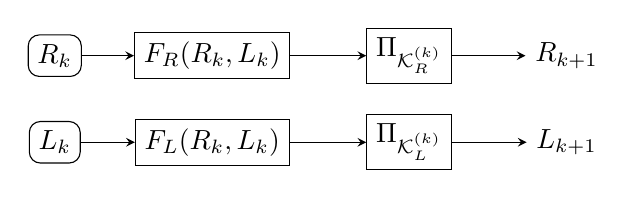
\begin{tikzpicture}[>=stealth, node distance=2.0cm]
\node[draw,rounded corners] (r) {$R_k$};
\node[draw,right of=r] (fr) {$F_R(R_k,L_k)$};
\node[draw,right of=fr,node distance=2.5cm] (pr) {$\Pi_{\mathcal K_R^{(k)}}$};
\node[right of=pr] (rn) {$R_{k+1}$};
\draw[->] (r)--(fr);\draw[->] (fr)--(pr);\draw[->] (pr)--(rn);
\node[draw,rounded corners,below of=r,node distance=1.1cm] (l) {$L_k$};
\node[draw,right of=l] (fl) {$F_L(R_k,L_k)$};
\node[draw,right of=fl,node distance=2.5cm] (pl) {$\Pi_{\mathcal K_L^{(k)}}$};
\node[right of=pl] (ln) {$L_{k+1}$};
\draw[->] (l)--(fl);\draw[->] (fl)--(pl);\draw[->] (pl)--(ln);
\end{tikzpicture}
\end{center}
两条更新通过混合环境耦合，但投影、规范化和变量分别保留。
每次投影量都记录；完整复数 $AC/C$ 残差及最终中心主根条件不变。
这是带对称性投影的独立双边固定点实验，尚不能仅凭对称性控制
宣布更大 $\chi$ 收敛。投影后的物理 RDM 仍需单独验收。

提交记录为 \path{antiunitary_pair_audit_submissions.json}、
\path{antiunitary_projection_retry_submissions.json}、
\path{antiunitary_seed_solver_v2_submissions.json}、
\path{antiunitary_projected_solver_control_submissions.json}。
新 \path{bare_antiunitary.py} 在原有 bare/direct 条件之外要求两方向
原始 RDM 的 trace、Hermiticity 和正性诊断通过；
\path{antiunitary_projected_control_validation_submissions.json}
记录了 $\chi=4$ 的存盘、RDM 和 bare 交叉验证链。
这些实验没有替换旧曲线，原生产求解器和 replica 后端保持原代码。

\subsection{投影迭代的小尺寸交叉验证与中心步长}
投影方法的非驻点 $\chi=4$ 控制已完成：独立扰动右边界后，
13 步达到完整残差 $6.07\times10^{-13}$，最终 $AC/C$ 均为主根。
存盘重验及两方向一至三格原始 RDM 检查通过。
作业 11356407、11356408 的 bare/direct 交叉验证得到
\begin{equation}
 \widetilde S_{\chi=4}=0.49038830734025396.
\end{equation}
该值与原控制相同；全部共同长度 $4,8,16,32,64,128$ 上，
两种计算的最大熵差为 $1.27\times10^{-13}$。
记录为 \path{independent_antiunitary4_bare_crosscheck.json}。
这验证了有限 $\chi$ 求解与收缩的一致性，仍不是 Gaussian 精度证明。

复 $\chi=16$ 分支投影后的\emph{初态}也完成物理检查：两、三格 RDM
Hermiticity 误差为 $1.77\times10^{-15}$、$1.27\times10^{-15}$，
trace 和正性诊断通过。但其完整方程残差仍为 $0.01584$，
所以不能把这个初态的 $\xi_{\rm pair}\simeq326.44$ 放进曲线。
不保持投影约束的中心跟踪作业 11356435 在第 3 步触发步长保护；
最好的仍是初态。带投影的作业 11356417 第一步残差为 $0.02446$，
第二步在\emph{局域候选的 gauge 对齐}中失败：重叠 cap 本征矢残差
$4.50\times10^{-15}$，但模长谱隙仅 $2.76\times10^{-14}$，
不满足原 $10^{-9}$ 的唯一性条件。它不是内层本征矢未算准，
也不能通过减小后面的 Anderson 步长来修复，因为异常发生得更早。

\path{anderson_antiunitary_damped_v2.jl} 因此增加一个更早的、有界中心步长。
对独立两侧分别由局域本征解 $(a,c)$ 构造
\begin{equation}
 a_\beta=(1-\beta)\frac{A_C}{\|A_C\|}+\beta a,
 \qquad
 c_\beta=(1-\beta)\frac{C}{\|C\|}+\beta c,
 \qquad \beta=1,\tfrac12,\ldots,\tfrac1{512}.
\end{equation}
先作原来的 regauge/canonicalization，再检查与各自当前态的 gauge 对齐；
若失败才减小 $\beta$。两侧都通过后，才进入原来的反幺正投影和
Anderson 候选步长 $\alpha$。$\beta$ 控制中心解到 MPS 的重建，
$\alpha$ 控制随后混合历史的更新，两者作用不同。
该变体记录每次失败与所选 $\beta$，并保存进入局域更新前的实际状态，
不放宽 cap、混合度量、完整复数方程、最终主根或 bare 验收条件。
独立的 $\chi=4$ 求解、存盘、物理及 bare 控制和有界 $\chi=16$
诊断提交在 \path{antiunitary_damped_v2_submissions.json}；提交本身不表示通过。
第一版在写入尝试记录时发生字典值类型错误（11356452），已保留错误日志；
v2 只扩展记录容器类型，并让意外的程序异常直接抛出，不能把它们归为
数值不收敛。旋转方向的原投影迭代也在第二步对齐失败（11356439），
模长谱隙 $1.62\times10^{-14}$。

v2 的四步 $\chi=16$ 诊断 11356471 已完成：第二步的 $\beta=1$
重复了原来的 cap 失败，$\beta=1/2$ 则通过。因此提前控制中心步长
确实绕过了这个已定位的异常；但四步的完整残差依次为
$0.02446,0.06597,0.07872,0.09789$，尚无收敛改善，最好仍为初态的
$0.01584$。该实验不产生新的熵或关联长度曲线点。

\subsection{实际失败步的重建连续性与 Newton 内层精度}
中心步长变体的完整 $\chi=4$ 验证链已经通过：存盘残差为
$5.96\times10^{-13}$，两方向原始 RDM 通过，bare/direct 结果
$0.49038830734025396$ 与旧控制一致（11356475、11356476）。
较长的投影 $\chi=16$ 试算 11356478 完成 50 个接受步，
第 51 步触发保护而停止；最好残差仍是初态的 $0.01584$。
故提前减小中心步长修复了一个候选构造异常，但未得到新的收敛环境。

另一项检查直接重放未施加投影约束的失败路线。
\path{anderson_targeted_trace.jl} 保持原算术流程，保存每步真实的
$R,L$ 和 Anderson 方向 $\Delta x$；11356619、11356623 验证重放
与原记录的初始及两个接受步一致，并重复第 3 步失败。
\path{audit_rebuild_continuity.jl} 检查
$x_\alpha=x+\alpha\Delta x$，分别在重新 canonicalize 和 gauge 对齐
前后计算完整方程，不调整验收门槛。

零步长控制 $\chi=4$ 的残差变化为 $5.79\times10^{-17}$。
实际 $\chi=16$ 失败前状态的零步长残差变化为
$7.93\times10^{-14}$，行商相对变化为 $1.08\times10^{-14}$。
这排除了该样本中的零步长重建错误。
$\alpha=10^{-4}$ 时完整残差从 $0.0334590$ 略降到 $0.0334445$；
$\alpha=1/1024$ 时则升到 $1.28583$。
同时，混合行通道的行商从约 $3.58250+0.00032i$ 变为
$0.13013+3.58037i$。这里检查的是行通道与重叠通道的本征值之比，
bare replica 的长度与相位仍单独验收。
提交记录为 \path{rebuild_continuity_submissions.json}。

随后沿\emph{这个实际方向}计算密集谱并连续标记本征值。
11356858、11356859 确认：两条行 cap 分支的模长在
$\alpha\in[3.5,3.6]\times10^{-4}$ 内交叉，按最大模选择的主根由
一条切换到另一条。采样点上，所跟踪本征值到其他本征值的最小相对
复平面距离仍为 $0.03574$，并非本征值合并；两侧本征矢残差检查通过。
因此，这个失败样本中的不连续来自\emph{按模排序后的根选择}，而非
零步长重建或内层本征矢精度不足。该样本不等同于旧曲线上的
$\chi=16$ 点，不能据此认定旧 $12\to16$ 的 $\xi$ 回落已有同一个因果解释。

\includegraphics[width=\linewidth]{../../code2d/fpeps/data/direct_chi_curve/independent_anderson_cap_branch16.pdf}

图及来源哈希为 \path{independent_anderson_cap_branch16.json}。
首个密集谱作业在节点上等待文件读取、CPU 时间接近零，取消后由
\path{anderson_cap_branch16_nfs_retry_submissions.json} 中的作业替代；
该基础设施失败未计入数值不收敛。

Newton 的另一个限制可在\emph{同一个冻结状态}上直接量化。
该状态来自 \path{native_antiunitary16_metric_newton_v2} 的最好迭代，
完整残差为 $9.10\times10^{-5}$，实切向坐标数为 1536。
\path{audit_krylov_capacity.jl} 不更新 MPS，只提高求解
$H\delta=-g$ 的 Krylov 子空间上限，并保留原解析导数检查。
作业 11356835 给出未施加步长限制时的线性相对残差：
\begin{center}
\begin{tabular}{r|rrrrrr}
子空间维数 &192&384&768&1024&1280&1464\\\hline
$\|H\delta+g\|/\|g\|$&0.7251&0.6870&0.6232&0.1626&0.003082&0.0008672
\end{tabular}
\end{center}
在 1464 维才达到原定的 $10^{-3}$ inexact-Newton 条件。
投影 Hessian 的非对称相对误差为 $2.12\times10^{-11}$；
有限步长的直接解析作用与小矩阵预测之差为 $6.47\times10^{-13}$。
但固定 trust radius 为 $10^{-5}$ 时，线性残差仍为 $0.9811$。
因此，提高内层精度消除了子空间容量限制，却不自动解决外层可接受
步长很小的问题，不能据此宣布方程收敛。

以 \path{newton_metric_krylov.jl} 的原实现、\path{maxbasis=1536}
作有限步续算，命令记录为 \path{krylov_full1536_submissions.json}。
对应 $\chi=4$ 求解控制 11356847 已通过，完整残差
$3.04\times10^{-12}$；存盘、物理及 bare 交叉验证亦已通过
（11356849--11356853）。$\chi=16$ 的完整方程是否收敛仍以最终报告为准。

基于上述实际 cap 交叉，再使用已有的解析分支跟踪实现
\path{newton_branch_krylov.jl}，并提高内层子空间上限至 1536。
已有的 $\chi=4,32$ 分支导数控制重新核对了来源哈希；实际失败前
状态另作四个独立左右、实虚方向的导数检查。
新的控制及有限步 $\chi=16$ 试算记录于
\path{branch_full1536_submissions.json}。
中间过程允许连续跟踪的 cap 暂时成为次主根，但最终仍要求原始
最大模 cap 审核、完整残差和物理检查通过。
这些提交不表示新环境已收敛，也不改变选定的熵和关联长度曲线。

\subsection{分别保持反幺正对称性的 Newton 切空间}
上述十步分支续算 11356870 已结束：最好完整残差为
$9.09883368\times10^{-5}$，最后一步为 $9.98614344\times10^{-5}$。
各存盘迭代的 cap 均为主根；分支梯度范数从 $0.01024$ 降到
$0.00861$，但完整方程并未同步改善。因此，这条续算的停滞不能
直接归因于主根切换，也未提供新的可接受熵点。
对应 $\chi=4$ 的完整 bare 验证链已通过，结果与旧值相差
$1.14\times10^{-13}$（11356869--11356875）。

下一变体针对先前出现的另一问题：复数驻点虽满足完整方程，其物理
RDM 仍可能不满足 Hermiticity。沿用已验证的反幺正作用，为两条
\emph{独立}边界分别求其虚空间 intertwiner，得到
$\mathcal K_R(A)=A$、$\mathcal K_L(B)=B$。这里不施加 $L=\mathrm{move}(R)$。
在每一侧的普通水平切空间中写
\begin{equation}
 \delta A=N_R V_R,\qquad A^\dagger N_R=0,\qquad
 \mathsf S_R(V_R)=N_R^\dagger\mathcal K_R(N_R V_R),
\end{equation}
左侧同理。以实坐标表示两侧直和作用 $\mathsf S$；当对称性保持该
切空间时，应有 $\mathsf S^T\mathsf S=I$、$\mathsf S^2=I$。
令 $Q_+$ 的列为其 $+1$ 子空间的实正交基。
这限制的是对称性允许的变化方向，不丢弃任何 Schmidt 方向，也不降低 $\chi$。

已有 Newton 坐标使用各边界自己的 Schmidt 变换 $x=P y$。
代码先数值检查 $\mathsf S P=P\mathsf S$，再验证完整梯度和 Hessian
满足 $g=Q_+Q_+^Tg$、$H\mathsf S=\mathsf S H$。
只有这些检查通过，才使用
\begin{equation}
 g_+=Q_+^Tg,\qquad H_+(v)=Q_+^T H(Q_+v),\qquad
 \delta x=P Q_+\delta y_+.
\end{equation}
极分解 retraction 的有限正负步也检查两侧反幺正对称性；解析 Hessian
作用与有限差分分别比较。控制采用非驻点，避免零梯度造成空泛通过。

作业 11357204、11357205 的检查通过：$\chi=4$ 的实切空间由
$96$ 限制为 $48$ 维，$\chi=16$ 由 $1536$ 限制为 $768$ 维；
最大对称性检查误差分别为 $5.32\times10^{-13}$ 与
$2.05\times10^{-11}$。四个左右、实虚方向中，最差的最佳 Hessian
有限差分相对误差分别为 $9.17\times10^{-9}$ 与 $5.49\times10^{-6}$。
这证明了这些样本上的切空间实现，不等于证明新求解器已经收敛。

实现为 \path{antiunitary_newton_chart.jl} 与
\path{newton_antiunitary_branch.jl}，提交记录为
\path{antiunitary_tangent_submissions.json} 和
\path{antiunitary_newton_control_submission.json}。
新求解器仍检查未投影的完整复数 AC/C 方程、最终主 cap 和主中心根。
物理 RDM、Gaussian 关联函数、bare/direct 长度及相位验收保持独立；
不能仅用受限方程的残差接纳环境。当前结果状态以相应最终报告为准。

\paragraph{接近零梯度时的检查与完整求解控制。}
第一版受扰动 $\chi=4$ 控制 11357208 将完整残差从
$9.05007\times10^{-3}$ 降至 $1.68969\times10^{-9}$，随后因
$\|(I-Q_+Q_+^T)g\|/\|g\|>10^{-8}$ 停止；这个结果尚未通过原有
$10^{-9}$ 环境门槛。冻结状态检查 11357213 测得
\begin{equation}
 \|g\|=1.37289\times10^{-8},\qquad
 \|(I-Q_+Q_+^T)g\|=1.54596\times10^{-14}.
\end{equation}
重新施加同一对称性后，张量系数相对变化为 $6.65\times10^{-16}$，
完整残差变化仅 $1.58\times10^{-15}$。因此这个样本的失败来自对
近零量使用纯相对检查，而非检测到显著的对称性破坏。
保留第一版及其失败记录，独立的
\path{newton_antiunitary_branch_v2.jl} 要求上述冻结状态证据及来源
哈希通过，并把\emph{梯度对称性诊断}改为
\begin{equation}
 \|(I-Q_+Q_+^T)g\|\leq 10^{-12}+10^{-8}\|g\|.
\end{equation}
完整复数方程的求解目标仍为 $10^{-11}$，环境、物理及 bare 验收
门槛均未改变；步长的 merit 仍包含未投影梯度的所有分量。

第二版 $\chi=4$ 控制 11357214 在四步后达到完整残差
$2.04621\times10^{-13}$，最终 cap 和 AC/C 中心根均为主根；
独立存盘检查 11357217 得到 $2.50305\times10^{-13}$。
物理与 bare 验证链记录于
\path{antiunitary_newton_v2_validation_submissions.json}；
其通过后才启动 $\chi=16$ 续算。
旋转方向另作独立切空间及种子 RDM 检查，命令在
\path{antiunitary_newton_rotated16_submissions.json}。
最终两方向存盘、物理谱、Gaussian 对照与 bare 测量的条件提交记录为
\path{antiunitary_newton16_measurement_submissions.json}。
提交记录不是大 $\chi$ 收敛证据，未通过的试算不进入选定曲线。

\subsection{较长关联长度的物理对照与每步对称性重投影}
第二版 $\chi=4$ 的物理及 bare 检查已通过：
$\widetilde S=0.49038830734025396$，与原值在报告精度内相同。
两个方向的 $\chi=16$ 二十步试算最好完整残差分别为
$8.61887\times10^{-5}$ 和 $8.63129\times10^{-5}$，均未收敛。
原方向试算的 $\xi_{\rm pair}=64.7185$、
$\xi_{\rm physical}=65.2900$ 只能作为未收敛状态的诊断值。
一至三格原始物理 RDM 在两个方向均通过检查，Hermiticity 误差
低于 $5.8\times10^{-15}$；这不证明整个无限态的正性。

与同一个 Gaussian 参照比较，较长的 $\xi$ 也不表示观测量全面改善。
例如 anomalous 关联在 $r=33\ldots128$ 的最大绝对误差由选定
$\chi=16$ 解的 $1.7721\times10^{-5}$ 降为 $3.8959\times10^{-6}$，
但在 $r=1\ldots8$ 由 $3.9205\times10^{-5}$ 增为
$8.8205\times10^{-5}$。短程 connected density 误差同样变大。
完整复数误差及分距离窗口的图保存在已有 \path{direct_chi_curve}
目录的 \path{independent_antiunitary16_trial_physical_comparison.*}。
该试算未进入选定熵或关联长度曲线。

\paragraph{在实际失败迭代上的数值检查。}
后续两个方向分别在第 5、10 步触发梯度对称性诊断而停止。
原方向的逐步存盘重放 11357395 重现了第 5 步的失败。
冻结该\emph{实际失败状态}后，11357397 测得
\begin{equation}
 \|g\|=0.00836771,\qquad
 \|(I-Q_+Q_+^T)g\|=1.19180\times10^{-10}.
\end{equation}
施加一次对称性重投影，张量相对变化为 $8.40\times10^{-15}$，
完整残差仅变化 $1.86\times10^{-14}$，而上述梯度分量降为
$3.47421\times10^{-11}$，通过\emph{未修改的}诊断门槛。
这说明该样本的检查对浮点量级漂移敏感，并不证明完整求解可以收敛。
另一个 Newton 初态接 Anderson 的试算在第四步停止，也未改善
已保存的最好完整残差。

\paragraph{第三版的操作及其限制。}
在每次 Newton 外层迭代开始，对每个独立边界自己的反幺正作用
$\mathcal K$ 作一次固定的重投影：
\begin{equation}
 A_0=\frac{A+\mathcal K(A)}{2},\qquad
 A_1=A_0(A_0^\dagger A_0)^{-1/2}.
\end{equation}
随后恢复混合正则形式，并把虚空间 gauge 对齐到 $A_1$。
左右分别操作；此步骤不把一条边界替换为另一条的方向变换。
要求最终系数相对原值变化不超过 $10^{-10}$，记录修正前后的
对称性及正则误差。每步只执行一次，不反复重算直到检查通过。
完整未投影梯度、原始 AC/C 方程、最终主根和 bare 验收均保持不变。
每步还保存当前两条边界、cap 分支参照及信赖域半径，以便从实际
失败位置继续，而不是总退回最好残差所在的旧迭代。

独立实现为 \path{newton_antiunitary_branch_v3.jl}，测量适配为
\path{bare_antiunitary_newton_v3.py}。提交记录为
\path{antiunitary_newton_v3_control_submission.json}、
\path{antiunitary_newton_v3_validation_submissions.json} 和
\path{antiunitary_newton_v3_pilot_submissions.json}。
第三版 $\chi=16$ 试算依赖该版本 $\chi=4$ 的完整求解、存盘、物理及
bare 对照链通过。其效果须查看最终报告，不能由修正量小推断收敛。

第三版受扰动 $\chi=4$ 控制 11357430 已通过：四步后完整残差为
$2.03239\times10^{-13}$，最终主 cap 及主中心根检查通过。
其后续存盘、物理与 bare 对照仍须分别验证。

\subsection{由双边局域重叠构造 Newton 预条件}
第三版的完整 $\chi=4$ 验证链已通过，bare/direct 熵与旧值相差
$1.14\times10^{-13}$。但单独逐步重投影尚不能解决 $\chi=16$：
原方向在续算第 5 步停止，完整残差 $9.41904\times10^{-5}$；
旋转方向在第 8 步停止，最后残差 $9.56206\times10^{-5}$。
两者仍由梯度对称性诊断触发停止，未获得新熵点。

另一个待检验因素是 Newton 的坐标缩放。原实现使用各自的
$(C C^\dagger)^{-1/2}$；它没有截断，但可能放大小 Schmidt 方向的
舍入误差。新的独立变体用\emph{两侧共同的局域 mixed overlap}
构造可逆预条件，仍求同一组完整驻点方程。

令 $A,B$ 为两条独立边界的左正则张量，
$\delta A=N_R V_R$、$\delta B=N_L V_L$，且
$A^\dagger N_R=B^\dagger N_L=0$。
在全部使用 $A,B$ 的 overlap 通道中求左右固定点 $l_0,r_0$，定义
\begin{equation}
 n_0=\langle B,(l_0\otimes I)A r_0\rangle,\qquad
 M(V_R)=\frac{N_L^\dagger(l_0\otimes I)N_R V_R r_0}{n_0}.
\end{equation}
分母消除两个 cap 的任意归一化和相位。实际矩阵仍由已有的 graded
收缩生成，不用忽略交换符号的普通 Kronecker 积替代。

\begin{figure}[htbp]
\centering
\begin{tikzpicture}[x=1.1cm,y=.8cm,>=Latex,
 t/.style={draw,rounded corners,minimum width=1.3cm,minimum height=.5cm},
 mixedcapbox/.style={draw,fill=gray!15,minimum width=.6cm,minimum height=1.6cm}]
 \node[mixedcapbox] (l) at (0,0) {$l_0$};
 \node[t,fill=blue!12] (a) at (2,.8) {$N_R V_R$};
 \node[t,fill=green!12] (b) at (2,-.8) {$\overline{N_L V_L}$};
 \node[mixedcapbox] (r) at (4,0) {$r_0$};
 \draw[->] (l.north east)--(a.west);\draw[->] (a.east)--(r.north west);
 \draw[->] (l.south east)--(b.west);\draw[->] (b.east)--(r.south west);
 \draw (1.86,.48)--(1.86,-.48);\draw (2.14,.48)--(2.14,-.48);
 \node[align=left] at (7,0) {网络除以 $n_0$：\\
 $\langle V_L,M V_R\rangle$\\两侧分别变分};
\end{tikzpicture}
\caption{不含 PEPS 行的局域双边切向量重叠。两条竖线是双层物理腿；
各腿的箭头、twist 和交换符号沿用前述空间约定。}
\end{figure}

这是\emph{局域}形式，不包含不同格点切向量间的全部响应，不能称为
完整 uniform-MPS fidelity 度量，也不等于整个 MPS 的双正交正则化。
对其系数矩阵 $M=U\Sigma V^\dagger$，有
\begin{equation}
 X=V\Sigma^{-1/2},\quad Y=U\Sigma^{-1/2},\quad Y^\dagger M X=I.
\end{equation}
为保留当前切空间坐标的方向，实际使用正 Hermitian 缩放
\begin{equation}
 P_R=V\Sigma^{-1/2}V^\dagger,\qquad
 P_L=U\Sigma^{-1/2}U^\dagger,\qquad
 P_L^\dagger M P_R=UV^\dagger.
\end{equation}
这里没有丢弃奇异向量；奇异值比低于 $10^{-12}$ 或白化误差不合格
就停止。在 $R=L$ 的极限，另检验 $M(V)=VCC^\dagger/\|C\|^2$，
在求逆之前检查该恒等式，以免弱权重掩盖方向约定错误。

将 $P_R,P_L$ 的实坐标表示记作直和矩阵 $P$。每个局域试步中固定
$P$，使用 $g_y=P^Tg_x$、$H_y=P^TH_xP$。先检验它与反幺正
切空间作用 $\mathsf S$ 对易，才能沿用 $Q_+$。主方程、最终主根及
观测量验收均不改变；预条件可逆也不意味着非线性迭代一定收敛。

冻结检查 11357456、11357457 已通过。$R=L$ 的密度恒等式误差
分别为 $1.13\times10^{-14}$、$1.55\times10^{-14}$。
在实际失败的 $\chi=16$ 状态上，新坐标的被丢弃梯度分量为
$1.32\times10^{-12}$，原坐标为 $1.19\times10^{-10}$；对应的相对量
分别为 $8.95\times10^{-10}$、$1.42\times10^{-8}$。
新坐标三个采样方向中最差的最佳 Hessian 有限差分相对误差为
$6.04\times10^{-6}$。这些是坐标实现的样本检查，不是收敛证据。

实现及定义在 \path{paired_tangent_metric.jl}、
\path{paired_tangent_metric.md}；独立求解版本为
\path{newton_antiunitary_paired_v4.jl}。
完整 $\chi=4$ 验证链通过后才运行两个方向的 $\chi=16$ 试算；
命令记录在 \path{antiunitary_paired_v4_*submissions.json}。
原方向仍从同一个失败状态开始，保留 cap 分支参照，
新坐标的初始信赖域半径显式设为 $10^{-3}$。
另以 \path{audit_paired_krylov.jl} 在同一冻结状态比较内层子空间，
同时报告原始、旧坐标和新坐标三种残差范数，避免仅因更换缩放
便误认为线性求解精度提高。

第四版受扰动 $\chi=4$ 控制 11357469 已在四步后通过，完整残差
$7.22517\times10^{-12}$，最终主 cap 和中心根检查均通过。
旋转方向的冻结坐标检查 11357475 也已通过；这些结果尚不能替代
完整物理、bare 检查或大 $\chi$ 收敛证明。

\subsection{候选边界的梯度响应与步长判据}
第四版的完整 $\chi=4$ 物理与 bare 验证链已通过，熵与旧结果相差
$1.14\times10^{-13}$。但两个方向的 $\chi=16$ 四十步试算均未收敛，
最好完整残差为 $8.50627\times10^{-5}$、$8.63129\times10^{-5}$。
冻结原方向第 21 步，检查 11357698 重现了被旧 merit 接受的一步：
旧坐标的梯度范数从 $4.26215\times10^{-4}$ 降至
$4.26149\times10^{-4}$，候选状态自身的原始水平梯度范数却从
$7.90643\times10^{-4}$ 升至 $7.94588\times10^{-4}$，完整残差也上升。
正则化对齐引起的张量变化低于 $1.6\times10^{-14}$。
这个结果说明旧坐标中余切向量的范数下降不保证换坐标后的方程改善；
它没有否定旧标量 pullback Hessian 的导数检查，也不是对选定
$\chi=12,16$ 两个曲线点的平台现象的原因证明。

\paragraph{固定坐标的 Hessian 与移动点的 Jacobian。}
对一条边界的左正则张量 $A$，令 $N^\dagger N=I$、
$A^\dagger N=0$。用水平坐标 $V$ 定义
\begin{align}
 A(V)&=(A+NV)(I+V^\dagger V)^{-1/2},\\
 N(V)&=(N-AV^\dagger)(I+VV^\dagger)^{-1/2}.
\end{align}
直接验证 $N(V)^\dagger N(V)=I$ 且 $A(V)^\dagger N(V)=0$。
记已有环境响应给出的 $\operatorname{Re}\log q$ 系数梯度为 $G$，
候选点的水平梯度为 $F(V)=N(V)^\dagger G(A(V),B(V))$。
在 $V=0$ 处，两侧分别满足
\begin{equation}
 J_F[V]=N^\dagger\mathrm dG-V(A^\dagger G),\qquad
 J_F[V]-H_{\rm pullback}[V]
 =-V\,\operatorname{skew}(A^\dagger G).
\end{equation}
其中 $\operatorname{skew}(K)=(K-K^\dagger)/2$；
$\mathrm dG$ 同时包含两个独立边界及四个 cap 的响应。
旧 Hessian 对应的第二项为 $-V\operatorname{Herm}(A^\dagger G)$。
离开驻点后，这两个导数对象不同，$J_F$ 也不必对称。
新的水平梯度范数等于
$\|G-A(A^\dagger G)\|_F$，不随正交补的幺正换基改变。

\paragraph{第五版的求根步骤。}
仍以局域 mixed-overlap 的可逆预条件 $P$ 和反幺正切空间基
$Q_+$ 建立搜索空间。对 $Q_+^T P J_F P Q_+$ 作非对称 Arnoldi，
得到正交列 $W$，同时保存原始响应矩阵
$D=J_F P Q_+W$。每步解
\begin{equation}
 \min_y\frac12\|F+Dy\|^2,\qquad
 \frac{\|y\|^2}{\Delta^2}
 +\frac{\|P Q_+W y\|^2}{\Delta_{\rm raw}^2}\leq1.
\end{equation}
预测与实际的下降量均使用\emph{原始}候选点水平梯度范数，包含
切空间投影外的分量。恢复正则形式后再核对该范数，才接受试步。
预条件只帮助寻找方向，不改变此 merit。最终仍须通过原始复数
AC/C 方程、主 cap、主中心根、物理 RDM 及 bare/direct 检查。
这是一种独立双边驻点方程的 Newton 求根实现，不等于整个 MPS
的双正交正则化，也不是调用包中现成的 bi-VUMPS 例程。

\paragraph{数值控制与保留的失败记录。}
非正规矩阵上的矩形最小二乘信赖域控制 11357735 与独立稠密 KKT
解一致，步长误差低于 $2.4\times10^{-15}$。
$\chi=4$ 的非驻点响应控制通过；$\chi=16$ 的四个独立侧随机方向
也通过，但原二阶差分在实际试步方向的小步长上失败。
高阶检查的四阶、六阶最佳原始相对误差为
$2.28\times10^{-6}$、$4.60\times10^{-6}$；两阶的全部加权误差
均低于原有 $10^{-4}$ 导数检查门槛。
附加的``相邻两个步长都满足原始误差 $10^{-5}$''规则仍未通过。
\path{point_gradient16_evidence.toml} 明确保留这一失败，另要求
每个阶数至少一个原始误差小于 $10^{-5}$、全部加权误差达标，
并核对随机方向与移动正交补检查。此诊断规则的调整不改变求解、
物理或熵验收门槛，不能把原失败报告改称通过。

第五版受扰动 $\chi=4$ 控制 11357750 在五步后达到完整残差
$8.68016\times10^{-14}$，最终主根检查通过。完整验证链和
原方向 $\chi=16$ 试算分别记录于
\path{antiunitary_point_v5_validation_submissions.json}、
\path{antiunitary_point_v5_native16_submission.json}。
定义、限制及复现命令索引见 \path{point_gradient_newton.md}。
大 $\chi$ 的结果必须以最终报告及物理、bare 对照为准，不能由
这个小 $\chi$ 控制外推；选定曲线没有因此新增点。

\subsection{直接以双边 AC/C 方程构造残差场}
第五版的完整 $\chi=4$ 验证链通过，bare 熵与旧值相差
$1.14\times10^{-13}$。但原方向 $\chi=16$ 二十步试算没有改善完整
方程：水平梯度范数由 $7.90643\times10^{-4}$ 降为
$2.78459\times10^{-5}$，完整残差却由 $1.07550\times10^{-4}$
升为 $2.05669\times10^{-4}$。已记录的四个追踪 cap 均为主根，也没有
触发对称性或试步异常。以下检查针对这条试算轨迹，不是选定
$\chi=12,16$ 曲线点之间相关长度变化的原因证明。

\paragraph{完整梯度仍需要正确的中心坐标。}
检查 11357882 发现，连未投影的原始梯度范数也下降约十倍，
而混合中心 AC 梯度的范数由 $0.04825$ 升至 $0.10721$。
令 $A_R,A_L$ 分别是两个独立态的左正则张量，$C_R,C_L$ 是它们
各自的中心矩阵；这里的 $R,L$ 表示双边变量，不表示同一态的
左右正则形式。原始梯度与实际中心梯度的关系为
\begin{align}
 G_{AC,R}&=G_R(C_R^\dagger)^{-1},&
 G_{C,R}&=A_R^\dagger G_{AC,R},\\
 G_{AC,L}&=G_L(C_L^\dagger)^{-1},&
 G_{C,L}&=A_L^\dagger G_{AC,L}.
\end{align}
在两个非驻点快照上，这与原始 AC/C pencil 算出的梯度在
$1.5\times10^{-8}$ 相对误差内相符。$C$ 的条件数只从约 $17566$
变为 $17841$；关键不是条件数突然变坏，而是梯度分量受到的
逆 Schmidt 权重与原始欧氏范数不同。接近驻点零值时另记录绝对
误差，不以相对误差膨胀冒充恒等式失效。

\paragraph{不截断的平滑度量与四个残差。}
对每一条独立边界，由自身范数通道求
\begin{equation}
 \mathcal E_{AA}(\rho)=\lambda\rho,\qquad
 \operatorname{tr}\rho=1,\qquad
 \rho=\frac{CC^\dagger}{\|C\|^2},\qquad W=\rho^{-1/2}.
\end{equation}
左正则时 $\lambda=1$。$GW$ 与 $G(C^\dagger)^{-1}$ 只差整体
标度和右侧幺正坐标，下面的归一化消去该标度。
$\rho_R,\rho_L$ 仅确定各自的正则坐标；$G_R,G_L$ 及响应仍来自
\emph{同一个双边带符号 PEPS 网络}，没有分别求解两套互不相关的
物理环境，也没有要求两条边界相同。

将原有 cache 的归一化两项写成 $G=H-N$，先令
\begin{equation}
 h=HW,\quad n=NW,\quad g=GW,\qquad
 s=\sqrt{\frac{\|h\|^2+\|n\|^2}{2}},\quad F_{AC}=g/s.
\end{equation}
对 $C$ 方程，把 $h,n,g$ 分别替换成
$A^\dagger h,A^\dagger n,A^\dagger g$ 后重新归一化。
合并两个独立方向的四个向量，使用
\begin{equation}
 \Phi=\frac12\left(\|F_{AC,R}\|^2+\|F_{AC,L}\|^2
                  +\|F_{C,R}\|^2+\|F_{C,L}\|^2\right).
\end{equation}
RMS 分母在 $H=N$ 附近平滑，与原始 max 分母最多差 $\sqrt2$。
它只用于选择试步；最终验收仍使用原始 max 归一化、双边白化
残差、主根、物理以及 bare/direct 检查。

\paragraph{必须求导 $W$ 和归一化。}
不能在候选点仅更换一次权重而仍使用旧响应。自身密度的变化由
带迹约束的线性方程给出：
\begin{equation}
 (\lambda I-\mathcal E_{AA})\,\delta\rho
 =(\delta\mathcal E_{AA}-\delta\lambda I)\rho,
 \qquad\operatorname{tr}\delta\rho=0.
\end{equation}
在 $\rho$ 的本征基底中，逆平方根的 Fr\'echet 导数为
\begin{equation}
 (\delta W)_{ij}=
 -\frac{(\delta\rho)_{ij}}
 {\sqrt{\rho_i}\sqrt{\rho_j}(\sqrt{\rho_i}+\sqrt{\rho_j})}.
\end{equation}
计算逐个 parity 块进行，不丢弃特征值或奇异方向。
完整响应包含
\begin{align}
 \delta g&=(\delta G)W+G\delta W,\\
 \delta(A^\dagger g)&=(\delta A)^\dagger g+A^\dagger\delta g,\\
 \delta s&=\frac{\operatorname{Re}(\langle h,\delta h\rangle+
                     \langle n,\delta n\rangle)}{2s},&
 \delta F&=\delta g/s-F\delta s/s.
\end{align}
非对称 Arnoldi 只建立搜索方向；信赖域最小二乘保留四个中心
残差的全部分量。恢复正则形式后重新计算实际 $\Phi$，再决定是否
接受试步。其实现为 \path{center_gradient_response.jl} 和
\path{newton_antiunitary_center_v6.jl}。

非驻点检查 11357898、11357899 已通过。$\chi=4,16$ 的中心场与
原始方程的对应误差分别为 $4.24\times10^{-12}$、
$1.79\times10^{-9}$；自身密度与 $CC^\dagger/\|C\|^2$ 的差异
低于 $1.2\times10^{-14}$。两侧各自的实、虚方向均作有限差分，
$\chi=16$ 最差的最佳场响应误差为 $1.06\times10^{-5}$。
这些检查验证实现与方程的对应关系，不能替代完整求解及熵验收。
定义与命令索引见 \path{center_gradient_newton.md}。

第六版受扰动 $\chi=4$ 控制 11357907 在五步后达到完整残差
$1.29643\times10^{-13}$，最终主 cap 及主中心根均通过检查。
旋转方向的场响应控制 11357908 也通过，最差的最佳有限差分误差
为 $9.07\times10^{-6}$。小 $\chi$ 的存盘、物理与 bare 验证链记录
在 \path{antiunitary_center_v6_validation_submissions.json}。
原方向 $\chi=16$ 仍从冻结的第四版第 21 步开始；旋转方向使用
其各自第四版的最终迭代快照。精确参数与两方向条件测量命令分别
在 \path{antiunitary_center_v6_native16_submission.json}、
\path{antiunitary_center_v6_rotated16_submission.json} 和
\path{antiunitary_center_v6_measurement_submissions.json}。
这些提交记录不代表大 $\chi$ 已收敛；两个方向的完整方程和物理
检查都通过后，才由条件任务继续 bare/direct 收缩。

\subsection{独立的 eig-CTMRG 子空间更新实验}
\label{sec:eigctm-pilot}

第六版的完整 $\chi=4$ 验证链已通过，bare/direct 熵为
$0.4903883073401403$，与选定点相差 $1.14\times10^{-13}$。
然而原方向和旋转方向的 $\chi=16$ 均停在对称响应检查，最佳完整
残差分别为 $7.77\times10^{-5}$ 和 $7.81\times10^{-5}$，因此均未
进入熵曲线。新的实验位于 \path{benchmark/eigctm/}，以
\href{https://arxiv.org/pdf/2609.05598}{arXiv:2609.05598}
第 V 节的 CTM 子空间条件为起点；其目标仍为独立左右变量的联合驻点。
以下描述试验实现，不表示大 $\chi$ 已收敛。

\paragraph{求解对象与开口。}
四个 enlarged corner 分别由旧 corner、两条旧 edge 和一个双层
PEPS site 收缩得到，记作 $Q_{\rm NW},Q_{\rm NE},Q_{\rm SE},Q_{\rm SW}$。
每条开口包含一个环境指标和 ket/bra 两条虚腿，总维数为 $\chi D^2$。
以西侧开口为基准，形成循环算子 $\Lambda$，并在该开口插入秩
$\chi$ 的投影 $\Pi$：
\begin{center}
\begin{tikzpicture}[x=1.15cm,y=.8cm,>=Latex,
 q/.style={draw,rounded corners,fill=blue!8,minimum width=1.3cm,minimum height=.7cm}]
 \node[q] (nw) at (0,2) {$Q_{\rm NW}$};
 \node[q] (ne) at (4,2) {$Q_{\rm NE}$};
 \node[q] (sw) at (0,-1) {$Q_{\rm SW}$};
 \node[q] (se) at (4,-1) {$Q_{\rm SE}$};
 \node[draw,fill=orange!12,minimum height=.65cm] (pi) at (0,.5) {$\Pi=V_RV_L$};
 \draw[->] (ne)--node[above] {$\chi D^2$} (nw);
 \draw[->] (se)--(ne);
 \draw[->] (sw)--(se);
 \draw[->] (nw)--(pi);
 \draw[->] (pi)--(sw);
 \node[align=center] at (2,.5) {循环收缩\\$Z(\Pi)$};
\end{tikzpicture}
\end{center}
图中的线性表示必须使用已经核对的 graded 指标约定；不能未经检验
就把图形闭合等同于无 twist 的普通矩阵迹。实现通过 PEPSKit 的
\path{EnlargedCorner} 和显式闭环张量收缩核对该对应。

\paragraph{双边子空间与平衡。}
在每个 parity 块中，保留模最大的 $\chi_q$ 维左右不变子空间。
令其正交基为 $Z_R,Z_L$，对交叠作
\[
 Z_L^\dagger Z_R=U\Sigma V^\dagger,\qquad
 V_R=Z_RV\Sigma^{-1/2},\qquad
 V_L=\Sigma^{-1/2}U^\dagger Z_L^\dagger.
\]
此处 $V_L$ 是行映射，已经包含 bra 的共轭约定，因而
\begin{equation}
 V_LV_R=I,\quad \Pi^2=\Pi,\quad
 \Lambda V_R=V_RK,\quad V_L\Lambda=KV_L.
\end{equation}
这里的 SVD 用来平衡两个已选子空间，不以其奇异值选择保留方向。
对 $K=V_L\Lambda V_R$ 再作幺正 Schur 旋转，可同时保持双正交条件
与 $V_R^\dagger V_R=V_LV_L^\dagger$。第一版是稠密的单个循环
Schur 求解，不声称已经实现 periodic Schur 或 block-Krylov 加速。
截断边界上的模简并、过小的交叠奇异值均显式报错，不暗中降秩。

对保持秩和投影性质的一阶变化 $\delta\Pi=[X,\Pi]$，在相应的线性
闭合约定下有
\[
 \delta Z=\operatorname{tr}(\Lambda[X,\Pi])
          =\operatorname{tr}([\Pi,\Lambda]X)=0.
\]
最初的 \path{audit_projector.jl} 通过了普通矩阵检查，但在实际
graded 闭环上失败，因而其原始循环算子不能用于物理试算。
非幺正相似变换下投影的协变性、拒绝拆开共轭本征值对等检查仍然
有效；它们只检验矩阵算法，不能代替以下图形与矩阵表示的核对。

\paragraph{费米闭环的矩阵表示与中性插入。}
将西侧开口记为 $W=V_\chi\otimes V_{\rm ket}\otimes V_{\rm bra}$，
其中每个因子保留其实际 dual 方向。定义在 $W$ 上的两个偶映射
\[
 J_W=\prod_{i:\,W_i\text{ 为 dual}}(-1)^{F_i},\qquad
 K_W=\prod_{i:\,W_i\text{ 为 nondual}}(-1)^{F_i}.
\]
它们作用在不同的指标上，均平方为一。固定本文的 TensorKit 图形
约定后，开放的图形连接与普通 block 矩阵乘法满足
$A\star B=A J_W B$。因此在这个开口上，图形的中性插入是 $J_W$：
$A\star J_W\star B=A\star B$。不能把普通矩阵 $I$ 直接代入。

令 $Q_{\rm raw}$ 是 \path{full_infinite_environment} 返回的开放
四角循环。对本文明确写出的闭环，使用的线性循环与图形投影为
\begin{equation}
 \Lambda=K_W Q_{\rm raw},\qquad
 P_{\rm graph}=J_W\Pi,\qquad
 P_L=J_WV_R,\quad P_R=V_L.
\end{equation}
于是显式闭环满足
\[
 Z(P_{\rm graph})=\operatorname{tr}(\Lambda\Pi),\qquad
 Z(J_W)=Z_{\rm unprojected}=\operatorname{tr}\Lambda.
\]
这里 $K_W$ 包含第一条环境腿 $\chi$；最初只处理 ket/bra 腿会漏掉
这一因子。旋转后 dual 方向改变，因此不能固定 twist 的位置。
\path{graded_cycle_v2.jl} 按实际腿方向计算 $J_W,K_W$。

该转换先通过独立的矩阵单位插入核对：对每个允许的 $E_{ji}$
直接收缩 $Z(E_{ji})$，得到线性形式 $M_{ij}=Z(E_{ji})$，再比较
$MJ_W$ 与 $K_WQ_{\rm raw}$。测试不使用 Gaussian 观测量选符号。
gapped、gapless 和无关随机复偶张量各取四个旋转方向，共十二组。
中性插入的开放网络差为零，闭环迹和分解投影误差约为
$10^{-16}$。旧的固定位置假设与漏掉 $\chi$ 腿的实现及失败报告均
保留。这些是代数和符号检查，还不是收敛环境的物理 benchmark。

\paragraph{外层迭代和验收。}
使用 $V_R,V_L$ 对旧西侧 edge 及其两端 corner 作增长和投影；
将网络和环境旋转后重复，四次构成一次完整 sweep。四方向的环境
数据分别更新，不从一条 MPS 镜像生成其余方向。
普通 SVD-CTMRG 仅提供已记录的初态。

局部投影残差小并不证明外层收敛。每个完整 sweep 提取相对的两条
edge MPS，分别恢复正则形式，将南向空间 MPS 通过已验证的
spatial-bra 映射转为 $L$，再调用不变的 \path{bv_audit} 检查双边
AC/C 方程；旋转方向独立作同样检查。连续三个 sweep 在两方向均
达到 $10^{-9}$ 才标记环境方程收敛。随后仍需物理 RDM、Gaussian
关联函数、主模及 bare/direct 长度和相位检查。
特别地，新的 CTM 方法不改变 $G=LR,B=LTR$ 的熵定义。

精确 Slurm 命令和源码哈希在
\path{data/eigctm_20260920/*submission*.json}。
第一版 11357962 在接口类型处失败；11357971 在实际 graded 闭环
上失败，驻点残差为 $1.47$，对应的物理试算未启动。
矩阵单位检查 11357988 完成十二组显式线性形式，但拒绝了跨所有
方向使用固定 twist 位置的假设。中性插入检查 11358010 通过，并
定位了遗漏的环境腿因子。修正后的实际投影与 CTM 更新接口检查
11358076 已通过：十二组中矩阵转换最大误差 $3.97\times10^{-16}$，
图形双正交最大误差 $5.02\times10^{-16}$，所有重整化张量有限。
因此启动了 11358077 的 gapped $\chi=4$ 试算；其外层与物理收敛
仍须独立检查。
精确命令在 \path{graded_v2_submissions.json}。
完整失败记录在 \path{graded_projector_diagnosis.md}。
第一轮 $\chi=4=(2,2)$ 试算被等模组截断检查拒绝：在两个 parity
块内，第二、第三个本征值等模，截断间隙约 $5.0\times10^{-17}$。
完整谱检查 11358090 确认四个方向均如此，因而随后独立运行
$\chi=6=(3,3)$，并保留同样的严格检查。

\paragraph{首个通过物理及 bare 检查的 gapped 点。}
$w=0.25,\chi=6$ 的作业 11358098 在七个 sweep 后，两方向最大
联合残差从 $2.73\times10^{-6}$ 降至 $1.60\times10^{-11}$，连续
三次通过 $10^{-9}$ 标准。存盘后重新检查两组独立边界，AC/C
驻点均为对应局部 pencil 的主模。这里普通单边 Galerkin 残差仍约
$2.92\times10^{-5}$，其原始未收敛标志保留；该数值与已经通过的
双边驻点条件不是同一验收标准。

两方向 $1,2,3$-site 原始 occupation RDM 的 Hermiticity 误差
均小于 $6\times10^{-16}$，最小本征值为正。物理关联谱能够重建
$r\leq64$ 的 normal、anomalous 与密度关联，误差小于 $10^{-15}$。
与 $2048/4096$ 网格 Gaussian 结果比较，$1\leq r\leq32$ 的最大
绝对误差分别约为 $4.37\times10^{-5}$、$3.97\times10^{-5}$ 和
$1.11\times10^{-6}$。这些是有限 $\chi$ 误差，不由方程残差代替。
相关长度分别为
\[
 \xi_{\rm MPS}^{R,L}\simeq1.47249208,\qquad
 \xi_{\rm pair}\simeq1.06065988,\qquad
 \xi_{\rm physical}^{\langle c^\dagger c\rangle}\simeq1.15153846.
\]
前者取单边 MPS 全 parity 谱；若仅取 even 通道，值为
$0.57409500$。密度关联的衰减长度及 residue cutoff 检查单独记录，
不与费米子关联的长度混用。

作业 11358120 通过未更改的 $G=LR,B=LTR$、有符号 replica、
character 对照、长度和相位检查，得到
\[
 \widetilde S_{\chi=6}=0.015944457360244968.
\]
终止深度为 32；三点长度漂移 $8.02\times10^{-9}$，深度 16 与 32
的直接差约 $5\times10^{-15}$，相位误差约 $3.15\times10^{-9}$。
Gaussian $L=32$ 环面结果除以四个交点后为
$0.01643014429301992$；$L=24\to32$ 漂移仅 $1.66\times10^{-9}$，
而本次有限 $\chi$ 熵误差为 $4.86\times10^{-4}$，约 $2.96\%$。
因此这是收缩稳定且物理一致的有限 $\chi$ 点，还没有达到高精度
Gaussian 熵 benchmark。数据在 \path{gapped_chi6_v2/}、
\path{gapped_chi6_physical/} 和 \path{gapped_chi6_bare/}。

固定 $(4,4)$ 的 gapped $\chi=8$ 试算初态已经不稳定，随后混合
度量病态，最终局部投影检查拒绝了该迭代；没有熵值。
另一版本 \path{global_space.jl} 按整个循环谱分配 even/odd 维数，
保持指定总 $\chi$，遇到无法分开的等模组仍报错。控制 11358122
对冻结初态和收敛 $\chi=6$ 环境的四个方向完成 24 项检查：
16 个允许的投影通过，8 个切开等模组的请求被正确拒绝。
在这些测试环境上，总 $\chi=4$ 选择 $(1,3)$，总 $\chi=6$ 选择
$(3,3)$，总 $\chi=8$ 的严格主模截断不允许。
条件试算 11358123--11358125 分别为 gapped $\chi=4$、gapless
$\chi=4,6$；这些提交不代表它们已经收敛。


\paragraph{首轮 global 试算：必须分开环境、物理和 replica 检查。}
gapped $\chi=4$ 的作业 11358123 在十三个 sweep 后达到两方向
最大联合残差 $2.12\times10^{-11}$，最终每个方向的 parity 维数
为 $(3,1)$。物理检查 11358138 通过，但 bare 检查 11358140
没有通过：长度增加到 1024 后，相位残差仍约为
$7.61\times10^{-8}$，大于未修改的 $10^{-8}$ 门槛。
因此其长度稳定的实数候选值不记作熵结果，也不加入选定曲线。
这个例子说明，双边方程和局域 RDM 通过仍不替代 replica 检查。

fresh gapless $\chi=4$ 的局域密度和 norm 已稳定，但原始联合
检查遇到不唯一的主 cap；$\chi=6$ 则在一百个 sweep 后仍有约
一的联合残差。作业 11358149 对前者的冻结环境和已验收的独立
$\chi=4$ 边界分别构造完整 even-cap 矩阵，没有为通过验收挑选
简并主空间中的某个向量。方向 0 的结果为
\begin{center}
\begin{tabular}{lcc}
\hline
通道 & fresh eig-CTM 主模重数 & 选定独立边界主模重数\\
\hline
单边 $R$ 自重叠 & 2 & 1\\
单边 $L$ 自重叠 & 2 & 1\\
双边 $LR$ 重叠 & 2 & 1\\
夹 PEPS 行的 $LTR$ & 4 & 1\\
\hline
\end{tabular}
\end{center}
谱的 backward residual 约为 $10^{-15}$，等模间隙约为
$10^{-15}$；这不是本征值求解精度不足。该方向的单边表示已经
不满足唯一主模条件。旋转方向的联合残差约为
$5.10\times10^{-15}$，不能代替方向 0 的失败。
对照的原独立边界联合残差为 $8.14\times10^{-13}$，其六个 cap
通道均有唯一主模。新旧方向 0 的 fidelity per site 约为
$0.998243$，因此不能将二者视为同一状态的可逆 gauge 变化。
完整报告为 \path{gapless4_peripheral/report.toml}。

\paragraph{保留已验收边界的暖启动。}
\path{pilot_seeded_global.jl} 新增两种明确的初值来源：
\texttt{paired\_caps} 使用独立求得的上、下 MPS，配合完整物理列
转移矩阵的左右主 cap 构成一个合法 CTM 初态；
\texttt{ctm\_snapshot} 直接续算已保存的四方向 CTM 数据。
前一种先检查上下 MPS 的 fidelity 和原始双边方程，且没有
SVD-CTMRG 预处理。初态的左右列 cap 不是已经优化好的水平
boundary MPS，仍需实际 CTM 更新后独立验收两个方向。
后续投影、等模组和原始残差标准均不改变。
精确命令在 \path{gapless_seeded_submissions.json} 和
\path{gapped4_polish_submission.json}；提交本身不代表通过验收。


\begin{figure}[htbp]
\centering
\includegraphics[width=\linewidth]{../../code2d/fpeps/data/direct_chi_curve/eigctm_gapless4_peripheral_spectrum.pdf}
\caption{被拒绝的 fresh gapless $\chi=4$ 环境和原独立边界的完整
cap 谱对照。橙色方向的多个 $|\lambda_j/\lambda_1|=1$ 不能用
增大传播长度消除；蓝色方向单独通过也不足以验收整个环境。
这里画的是 even-cap 谱，不是全 parity 的单边 MPS 关联长度。}
\end{figure}

第一轮暖启动中，gapless $\chi=4$ 的上下 MPS fidelity 误差
小于 $5\times10^{-16}$，初始上下双边残差为
$8.14\times10^{-13}$；完整四方向初态尚未收敛。
实际更新一百轮后，联合残差降至 $1.23\times10^{-8}$。
续算 11358163 又经过十九轮，达到 $7.17\times10^{-10}$，连续
三轮通过原门槛。随后的物理作业 11358171 和 bare 作业 11358173
均通过，得到 $\widetilde S=0.4903883060571843$；与原独立双边
结果之差为 $-1.28\times10^{-9}$。单边及双边相关长度也复现原解。
该比较验证两种更新算法找到相同的有限 $\chi$ 解，不意味着
$\chi=4$ 已达到精确 Gaussian 极限。

$\chi=6$ 的 global 暖启动在第一轮把已验收初态的 $(4,2)$
换成了 $(3,3)$，一百轮后残差为 $0.0110$ 且仍在漂移。
因此另保留 \path{pilot_seeded_fixed.jl} 对照，固定 $(4,2)$ 表示，
每个 parity 块内仍使用完整不变子空间及原严格截断检查；它不被
描述为全谱按模最大的六个模式。该对照用于区分 parity 维数
重新分配与迭代本身的失稳，不能预先认定能收敛。

从已收敛 gapped $\chi=6$ 四方向 CTM 初态直接增长到 $\chi=10$
和 $12$ 的两项试算（11358164 和 11358165）均在十轮后通过原联合方程，
最大残差分别为 $2.12\times10^{-11}$ 和 $2.81\times10^{-11}$，
最终 parity 维数分别为 $(4,6)$ 和 $(6,6)$。这些是实际总维数。
物理、Gaussian 和 bare 测量分别提交；尚不能把环境残差当作熵
精度。原严格全谱检查在冻结 $\chi=6$ 初态拒绝了 $\chi=8$ 的
切开等模组请求，因而这次没有伪造一个 $\chi=8$ 点。


\paragraph{完成测量的 gapped 系列。}
$\chi=10,12$ 的两方向原始 RDM、完整物理 cap 和关联函数重建
均通过；bare 作业 11358176/11358179 保留原 $G=LR,B=LTR$、
有符号 replica 及全部长度、相位门槛。数据如下；单边左右 MPS
长度在所示精度相同。
\begin{center}
\begin{tabular}{rrrrrr}
\hline
$\chi$ & $\widetilde S$ & $\xi_{\rm MPS}$ & $\xi_{\rm pair}$ &
$\xi_{\rm physical}$ & Gaussian 相对误差\\
\hline
6 & 0.01594445736 & 1.472492 & 1.060660 & 1.151538 & $2.956\%$\\
8 & 0.01593365896 & 1.472776 & 1.060421 & 1.151380 & $3.022\%$\\
10 & 0.01657716591 & 1.330864 & 1.209437 & 1.227014 & $0.895\%$\\
12 & 0.01655454854 & 1.348294 & 1.198160 & 1.219350 & $0.757\%$\\
\hline
\end{tabular}
\end{center}
$\xi_{\rm physical}$ 由 normal 费米子关联的非零 residue 模式
取得。Gaussian 基准仍为 $L=32$ 环面除以四个交点，尺寸漂移
$1.66\times10^{-9}$；表中的有限 $\chi$ 误差明显更大。
两新点的终止传播深度均为 32，长度漂移分别为
$4.32\times10^{-8}$、$3.83\times10^{-8}$。
$\chi=10$ 的相位误差 $9.84\times10^{-9}$ 接近 $10^{-8}$ 门槛，
只按原标准记录通过，不额外声称高精度；$\chi=12$ 为
$1.35\times10^{-10}$。

gapped $\chi=4$ 的补充迭代虽把环境残差降至
$2.17\times10^{-13}$，bare 相位仍为 $7.61\times10^{-8}$。
因此该失败不能归因于外层提前停止，此点继续排除在熵曲线外。

\begin{figure}[htbp]
\centering
\includegraphics[width=\linewidth]{../../code2d/fpeps/data/direct_chi_curve/eigctm_gapped_bare_chi_with8.pdf}
\caption{新 eig-CTM 路线在 $w=0.25$ 的 bare/direct 数据、Gaussian
误差和三类相关长度。横轴为 $\log\chi$；没有插入未通过验收的点。
文件和 CSV 位于原 \texttt{data/direct\_chi\_curve/}，作为独立系列保存。}
\end{figure}

\paragraph{完整等模组与精确指定秩。}
固定 $(4,2)$ 的初次对照 11358170 仍在第一步失败，截断处模间隙
为 $2.38\times10^{-13}$。新的 \path{whole_clusters.jl} 不降低
该检查门槛，而把相邻模差低于 $10^{-12}$ 相对谱半径的模式分成
完整组。必须保留主组；其余按模优先，在保证剩余组可恰好填满
维数时保留一整组，否则跳过该组。不存在恰好填满指定秩的选择
就报错，没有隐式降秩。它保留的可能不是最大的前 $\chi$ 个模，
该差别在每步元数据中明确记录。

\path{oblique_whole_schur.jl} 对选定的完整左右 Schur 子空间使用
相同双正交化，并继续检查 $V_LV_R=I$、投影幂等性、与循环矩阵
的交换子及左右不变子空间残差。独立控制 11358185 包括非酉
similarity 下的投影协变、禁止切开主组、精确维数分配，以及
两个实际冻结环境的四个方向。八组 graded 图形检查最大误差
$4.06\times10^{-16}$，全部通过。之后才启动
\path{pilot_seeded_whole.jl} 的 gapless $(4,2)$ 与 gapped $(4,4)$
条件试算；这些代数控制不代替外层、物理或 bare 验收。

两项条件试算随后都通过原双边方程：gapless $\chi=6=(4,2)$
的 11358190 在 97 轮后残差为 $6.71\times10^{-10}$；
gapped $\chi=8=(4,4)$ 的 11358191 在八轮后为
$2.42\times10^{-11}$。物理和 bare 验收另见
\path{whole_smallchi_measurement_submissions.json}，这里尚不报告
这两点的熵。基于新的 gapless $\chi=6$ 四方向 CTM 初态，
进一步增长至 $\chi=8$ 的提交在 \path{gapless8_whole_submission.json}。


\paragraph{完整等模组试算的测量结果。}
前述 gapless $\chi=6$ 的物理和 bare 作业 11358200--11358202
均已通过，得到
\[
\begin{aligned}
 \widetilde S&=0.5344557026637631,\\
 \xi_{\rm MPS}^{R}&=1.17798195545,\qquad
 \xi_{\rm MPS}^{L}=1.17798195565,\\
 \xi_{\rm pair}&=3.71979119277,\qquad
 \xi_{\rm physical}=4.24867923461.
\end{aligned}
\]
与原独立双边解的熵差为 $-1.23\times10^{-9}$，所有相关长度
之差小于 $2.1\times10^{-8}$。这是算法间的有限 $\chi$ 复现；
normal 关联函数与 Gaussian 的最大误差仍约 $0.00770$，不把
驻点精度等同于精确态精度。

gapped $\chi=8$ 的物理和 bare 作业 11358203--11358205 也通过，
\[
 \widetilde S=0.015933658962836716.
\]
长度漂移为 $6.00\times10^{-9}$，相位误差 $4.69\times10^{-15}$。
Gaussian 相对熵误差约 $3.022\%$，略大于 $\chi=6$。
表和新版本图如实保留该非单调性，没有以收敛性筛选出单调曲线。
原独立求解器的选定数据及早期 eig-CTM 图均未覆盖。

\paragraph{四方向同时更新：投影兼容性与外层收敛是两项检查。}
逐方向更新的 gapless $\chi=8$ 从新 $\chi=6$ CTM 出发，150 轮后
联合残差为 $0.08090$；从原选定 $\chi=8$ 边界初态出发同样不稳定。
因此另实现 \path{simultaneous_whole.jl}：在同一份冻结环境上
构造四个 enlarged corner 和四个 cyclic cut 的完整不变子空间。
令 $\Pi_i=V_{R,i}V_{L,i}$ 表示线性图表下的投影；在实际 graded
图中使用已验证的 twist，并逐个检查
\[
 \Pi_i\star C_i=C_i\star\Pi_{i+1},\qquad i\pmod4.
\]
这里 $\star$ 表示带方向和费米子 twist 的图形收缩，不是忽略
方向的普通矩阵乘法。所有相对残差低于 $10^{-9}$ 后才同时
重整化四个 corner 和四个 edge。四条边独立保留，不从某一条
边镜像复制其他边。当前实现对四个循环分别作稠密 Schur 后检查
兼容性，尚不是文中的 periodic Schur 或 block-Arnoldi 实现。

控制作业 11358226 对已收敛的 gapped $\chi=6$、gapless
$\chi=4,6$ 各更新一步。四条 edge 的 fidelity 误差均小于
$3.4\times10^{-15}$，周期兼容性残差不超过 $1.43\times10^{-12}$，
原始双边方程继续通过。
然而条件试算 11358239 从 gapless $\chi=6$ 扩张至 $8$，150 轮
之后仍振荡，残差为 $0.11542$。从原选定 $\chi=8$ 初态出发的
11358238 则在第二轮之前因一项兼容性残差为
$1.095\times10^{-9}$ 而停止，没有放宽门槛。
这两次失败不产生熵点。

\paragraph{经过 gauge 对齐的阻尼对照。}
记全部 CTM 数据为 $X$，同时更新映射为 $F(X)$。直接混合不同
虚拟基底下的张量没有明确意义，因此先把各张量范数归一，利用
PEPSKit 的 \texttt{ScramblingEnvGauge} 把 $F(X_n)$ 的酉 gauge
对齐到 $X_n$，再作
\[
 X_{n+1}=\mathcal N\!\left[(1-\alpha)\mathcal N(X_n)
       +\alpha\,\mathcal N\bigl(g_n\cdot F(X_n)\bigr)\right],
 \qquad 0<\alpha\leq1.
\]
$\mathcal N$ 表示逐张量范数归一；$g_n$ 仅作 gauge 对齐，后面的
线性混合才改变迭代。它不声称用 gauge 变换改变同一状态的
$\xi$。增大 $\chi$ 的第一步因虚拟空间不同而明确跳过混合。

控制作业 11358242 在上述三个已知驻点检查对齐前后的 norm、
密度和四条 edge fidelity，误差约为 $3.2\times10^{-15}$ 以下；
对齐后的最大逐张量差为 $9.94\times10^{-9}$，混合后原始联合
方程仍通过。这个控制验证了所测驻点附近的酉对齐，不保证对
任意病态非酉 gauge 都有效。实际 pilot 每步重新检查对齐不改变
环境的标量收缩；$\alpha=0.2,0.5$ 的条件提交为
11358246、11358247。外层仍须连续三轮通过两方向 $10^{-9}$
原始联合残差，之后才允许物理及 bare 流程。
完整命令在 \path{damped_conditional_submissions.json}；命令数组
应在 fPEPS 目录运行，并使用新的输出路径以免覆盖已有结果。


两项阻尼首轮随后均完成但未通过：$\alpha=0.2$ 的 300 轮最终
残差为 $0.0236679$，$\alpha=0.5$ 为 $27.1532$。各步局部投影
代数残差始终小于 $3.4\times10^{-14}$。因此这里已经能够区分
局部不变子空间求解精度与外层固定点迭代稳定性。
较小阻尼在最后阶段仍有下降趋势，单独续算 400 轮的提交为
11358298；是否达到原门槛必须另行检查。
\begin{figure}[htbp]
\centering
\includegraphics[width=\linewidth]{../../code2d/fpeps/data/direct_chi_curve/eigctm_gapless8_update_diagnostics.pdf}
\caption{同一 gapless $\chi=6$ CTM 初态扩张至 $\chi=8$ 后的四种
更新方式。左：原始联合残差；中：包含虚部的密度偏差；右：
最大斜投影谱范数。横轴从扩张后的第一轮开始。叉号在 $10^3$
处标记无法通过 cap 审核的轮次，不代表残差恰为 $10^3$。
这四次首轮试算均未通过原 $10^{-9}$ 外层门槛。}
\end{figure}

\paragraph{文中式 (57) 的边界字典：隔离的初始化检查。}
在原 \texttt{paired\_caps} 初态中，水平 edge 使用完整 $LTR$
通道的左右 cap，corner 为单位映射；这些 cap 可保持原上下边界
的物理行收缩，但并未被声明为已优化的水平 MPS。
文中式 (57) 的 CTM 字典还含有 $LR$ 重叠 cap 的逆。
新的 \path{audit_mpbp_pair_dictionary.jl} 将该重叠因子移到
相邻 corner，再由物理 cap 除以它构造水平 edge。
实际实现显式保留内部 dual 腿的 twist；先验证缝合后的完整物理
cap 与原初态逐元素相同，才检查新水平边界的驻点方程。
任何不可逆或相对奇异值低于 $10^{-12}$ 的重叠因子都会被拒绝，
没有以伪逆截断静默改变状态。
该作业 11358253 是零优化步的转换检查，没有修改生产初值函数，
也没有预先把所得环境当作已收敛。完整命令在
\path{pair_dictionary_submission.json}。


转换控制 11358253 随后对原 gapless $\chi=4,6,8$ 三组独立
上下边界全部通过。两方向原始联合残差的最大值分别为
$8.14\times10^{-13}$、$1.30\times10^{-12}$ 和
$5.16\times10^{-12}$；优化步数严格为零，上下 edge 张量逐元素
不变。完整物理 cap 的缝合误差最大为 $4.05\times10^{-14}$，
密度变化最大为 $5.67\times10^{-15}$，所测重叠 cap 最小相对
奇异值为 $5.02\times10^{-4}$。
因此水平边界可以由两个独立相对边界的驻点数据经该字典导出，
再独立验算其方程；这不是镜像猜测，也不声称四条 MPS 都经过
单独的数值优化。

该结果定位的是旧暖启动的不足：它保持物理行收缩，却没有
直接处于完整四方向驻点。它不推翻之前保持不变的上下边界
bare/direct 熵。新的转换已经给出已知 $\chi=8$ 解的四方向表示，
但所选 eig-CTM 更新能否保持及稳定吸引这个驻点仍是下一项检查。
作业 11358300 测试一步更新，11358301 对原 $\chi=12,16$ 边界
测试同一零优化步字典；未据此宣称得到新大 $\chi$ 熵。


以代码中西边为例，$h_W$ 为 $LTR$ 的左 cap，$g_W$ 为 $LR$ 的左 cap。
$h_W$ 的末腿及 $g_W$ 的定义域属于北边虚拟空间 $V_N$，
$g_W$ 的值域属于南边虚拟空间 $V_S$。令
$J_N=\mathrm{twistdual}(I_{V_N})$、
$J_S=\mathrm{twistdual}(I_{V_S})$，该图表中的实际矩阵表达式为
\[
 W_{\rm new}=h_W J_N g_W^{-1}J_S,\qquad
 C_{NW}=g_W,\qquad C_{SW}=I_{V_S}.
\]
东边由对应右 cap 作同样构造。因为图形复合在内腿插入相应的
$J$，必须验证的是
\[
 I_{V_S}\star W_{\rm new}\star g_W
   = I_{V_S}\star h_W\star I_{V_N},
\]
而不是从无向 bosonic 矩阵图直接省略这些符号。
\begin{center}
\begin{tikzpicture}[x=0.9cm,y=0.8cm]
\node[draw,rounded corners,minimum width=1.1cm,minimum height=0.6cm] (h) at (0,0) {$h_W$};
\draw (-1.4,0)--(h);\draw (h)--(1.4,0);
\draw (-0.2,-0.3)--(-0.2,-0.9);\draw (0.2,-0.3)--(0.2,-0.9);
\node at (-1.25,0.35) {$V_S$};\node at (1.25,0.35) {$V_N$};
\node at (2,0) {$=$};
\node[draw,rounded corners,minimum width=1.2cm,minimum height=0.6cm] (w) at (3.7,0) {$W_{\rm new}$};
\node[draw,minimum width=0.8cm,minimum height=0.6cm] (g) at (5.7,0) {$g_W$};
\draw (2.5,0)--(w);\draw (w)--(g);\draw (g)--(6.9,0);
\draw (3.5,-0.3)--(3.5,-0.9);\draw (3.9,-0.3)--(3.9,-0.9);
\node at (2.65,0.35) {$V_S$};\node at (4.75,0.35) {$V_S$};\node at (6.75,0.35) {$V_N$};
\node at (0,-1.3) {物理行 cap};\node at (4.7,-1.3) {水平 edge 与 corner};
\end{tikzpicture}
\end{center}
图中两根下伸线是原 PEPS 行的 ket/bra 虚拟腿；省略了两端单位
corner，所有接线按上式的 graded 收缩解释。$g_W^{-1}$ 的作用是
把原先不同边界的虚拟空间接成可沿水平方向重复的 MPS。


\paragraph{后续控制：驻点与当前选谱更新的固定点必须区分。}
$\alpha=0.2$ 的 400 轮续算 11358298 仍失败，最终残差为
$19.1656$，因此不能把前 300 轮末尾的暂时下降解释为渐近收敛。
零优化步转换 11358301 对 $\chi=12,16$ 通过；两方向最大残差
分别为 $8.87\times10^{-12}$、$1.10\times10^{-10}$，完整物理 cap
缝合误差分别为 $7.54\times10^{-15}$、$5.97\times10^{-13}$。

但 $\chi=8$ 一步更新控制 11358300 没有保持原驻点：联合残差从
$5.16\times10^{-12}$ 变为 $0.00962618$，四条 edge 的 fidelity
误差均约 $2.9953\times10^{-5}$。投影周期兼容性仍通过，最大
残差约 $1.43\times10^{-11}$。这说明原始边界方程驻点不能直接
当成当前按模选子空间更新的固定点，不能只归因于初态差或
浮点误差。可能涉及保留子空间切换，也可能仍有待检查的 CTM
一致性条件；这一步测试本身不区分两者。

文中式 (36)--(47) 将驻点保留的 corner 循环谱视为 enlarged
循环谱的一个子集；保留最大模是算法选择，而不属于驻点定义。
作业 11358305 因而比较小 corner 循环与完整 enlarged 循环的
本征值，显式记录共同尺度的假设、逐模匹配误差和是否为按模
排序的前 $\chi$ 个模式。这是对更新失败的诊断，不是新的熵点。


谱诊断 11358305 完成。对 $\chi=4,6,12$，已知驻点的小 corner
循环谱匹配到各 parity 块完整循环谱的前若干个最大模。
$\chi=8$ 则在 odd 块匹配到排序编号 $\{1,2,3,5\}$，而不是
$\{1,2,3,4\}$；最大逐模相对匹配误差为 $6.96\times10^{-11}$。
该块的第四、第五个归一化本征值约为
$1.72069099\times10^{-4}$ 与 $1.33087442\times10^{-4}$，
两者并不简并，因此仅保持完整等模组不能消除这一选择差别。
$\chi=16$ 的 even 块匹配到 $\{1,2,3,4,5,6,7,10\}$，odd 块
匹配到 $\{1,2,3,4,5,6,8,9\}$；最坏逐模相对误差约
$2.86\times10^{-9}$，保留其较差的条件数说明。

这给出一个可检验的子空间切换解释，但仍不证明原有限 $\chi$
驻点是全局最优，或新的最大模分支具有更小 Gaussian 误差。
\path{reference_cycle_projectors.jl} 因而仅作冻结驻点对照：以旧
corner 循环谱匹配左右 Schur 子空间，检查匹配唯一性、完整等模
组、双正交与不变性，再执行完全相同的四方向更新。
它要求参考谱已经匹配、且保持同一秩，尚不是增大 $\chi$ 或处理
未收敛环境的通用算法。小、大 $\chi$ 对照提交为
11358384、11358385；验收检查更新后的原始双边方程及四条 edge
fidelity，而不使用熵曲线作为选谱依据。


参考子空间对照 11358384 对 $\chi=4,6,8$ 全部通过。
其中 $\chi=8$ 更新后的原始联合残差为
$5.07\times10^{-12}$，四条 edge 的最大 fidelity 误差为
$3.11\times10^{-15}$。与最大模子空间对照相比，仅选择改变便
决定了这一轮是否保持原边界。因此该 $\chi=8$ 一步偏离的来源
已经定位到选谱，而不是尚未收敛的初态或纯 gauge。
大维数对照 11358385 中，$\chi=12$ 同样通过，更新后残差
$8.60\times10^{-12}$、fidelity 误差不超过 $5.33\times10^{-15}$。

$\chi=16$ 在另一 cyclic cut 的最小保留模遇到参考谱相对匹配
误差 $4.13\times10^{-8}$，超过该诊断先设的 $10^{-8}$，因此
11358385 在更新前拒绝了它。这个门槛用于辨认谱分支，不是
原始双边方程的收敛门槛。另保留
\path{reference_cycle_projectors_separation.jl} 对照：匹配偏差
必须同时小于谱半径的 $10^{-12}$，以及该模至最近其他本征值
距离的 $10^{-3}$。这样直接检查匹配是否能分辨，避免只因本征值
较小就误判其分支。原等模组、投影代数、周期兼容性、方程残差
和 fidelity 检查不变。作业 11358387 先验证已知微小孤立模的
投影，并拒绝不匹配和模间歧义两个反例，再对五个冻结驻点
作对照；失败版本和诊断数据均保留。


分离度版本 11358387 的三个矩阵控制以及 $\chi=4,6$ 通过，
但在 $\chi=8$ 更新前被其试设的 $10^{-12}$ 谱半径门槛拒绝：
最大参考匹配偏差为 $4.95\times10^{-12}$，而相对最近其他模式
的误差不超过 $2.37\times10^{-10}$，匹配本身仍清晰。
该版本不提升为正式求解器；后续参考匹配需同时考虑输入驻点的
有限残差与小模式的条件数。原版本已完成的 $\chi=8,12$ 一步
fidelity 对照独立保留，$\chi=16$ 尚无完成的一步更新验收。
没有为接纳某个熵点修改原始物理或外层门槛。

最后，作业 11358388 从已通过两方向方程及一步对照的
$\chi=12$ 字典快照开始完整 simultaneous whole-group 迭代，
仍要求连续三轮通过原联合残差。其完整命令在
\path{gapless12_dictionary_submission.json}。
这次提交不代表已取得新熵，也不代表 $\chi=16,24,32$ 已稳定。


\paragraph{$\chi=12$ 完整迭代的确认。}
11358388 随后连续三轮通过原始双边方程，最终残差为
$1.0692\times10^{-11}$。单边左右 $\xi_{\rm MPS}$ 分别为
$6.10022484275$、$6.10022484263$，$\xi_{\rm pair}=25.4980753737$。
这些是保存环境后重新计算的谱，物理关联长度还须由独立测量
确认。物理、Gaussian 关联、bare 及原 $\chi=12$ 数据对照提交
分别为 11358408、11358410、11358411、11358412；从这份已收敛
四方向快照扩张到 $\chi=16$ 的提交为 11358413。
命令及哈希在 \path{dictionary12_measure_and_grow16_submissions.json}。
测量和大维数试算的完成状态不能由本段提交记录代替。


\paragraph{$\chi=12$ 的物理及 bare 复现完成。}
11358408 的两方向原始 RDM 和完整物理关联谱检查通过，
normal 关联的 $\xi_{\rm physical}=26.0317237754$，Gaussian
关联函数最大误差为 $0.00148245636$。bare 作业 11358411 按原
$G=LR,B=LTR$ 传播至深度 1024，通过长度与相位检查，得到
\[
 \widetilde S_{\chi=12}=0.765262255316884.
\]
没有使用 grown tensor 或 endmap。对照 11358412 与原选定
独立双边 $\chi=12$ 解的熵差为 $+3.73\times10^{-11}$，所有
相关长度之差小于 $1.1\times10^{-9}$。这是同一有限 $\chi$ 解的
独立更新算法复现，不是精确 Gaussian 熵极限的认证。
原选定曲线保持不变。$\chi=16$ 扩张作业 11358413 曾因账户额度
\texttt{AssocGrpBillingMinutes} 排队，随后已启动；排队时间
不是数值不收敛。新 $\chi=16$ 的方程、物理和 bare 验收仍须
独立完成。



\section{旧路线存档：受方向约束的求解器不是严格的双正交 VUMPS}
\label{sec:biorthogonal-correction}

本节及其后续旧表格记录 2026-09-19 以前的路线；其中“当前”均为历史语境。
新的独立左右实现见第~\ref{sec:independent-bivumps} 节，不继承本节的数值认证。
这里必须把旧文档中的“双边 VUMPS”改成更准确的说法。旧路线代码
\code{selected\_precision\_weighted\_trust.jl} 解的是一个
target-$\chi$ 的\emph{耦合边界残差问题}，并不是图~\ref{fig:bi-vumps-flow}
所示的标准 bi-VUMPS。代码用一个参数化的基张量 $a$ 生成
$S=\mathrm{native}(a)$ 和 $R=\mathrm{move}(S)$，然后在每个 trial 点分别求
左右 cap 的主固定点，构造 $H_{AC},N_{AC},H_C,N_C$，驱动受约束参数的更新，
并用完整 joint residual 验收。因而
\begin{equation}
  R=\mathrm{move}(S)\quad\text{是当前模型方向约束，}
  \qquad\text{不是独立的左右 fixed-point 解。}
\end{equation}

这解释了为什么当前代码中会看到
\code{joint\_leading(transfer\_left)} 和
\code{joint\_leading(transfer\_right)}：它们是给定候选边界后的 cap/effective
channel 求解，不等价于先求出 transfer MPO 的独立左、右 MPS 主固定点。
代码也没有对左右 MPS 的中心重叠矩阵做一次独立的
$Q_L^\dagger Q_R=U\Sigma V^\dagger$ SVD，再把左右虚基变换到
$\widehat Q_L^\dagger\widehat Q_R=I$。因此当前的
\code{metric\_condition}、\code{metric\_inverse\_error} 和 joint residual
不能被解释成 biorthogonal gauge 的收敛证据。

还需纠正此前的流程描述：不必先把左右 ordinary VUMPS 各自完全求收敛，
再作一次重叠 SVD。独立左右态可以从初态开始一起迭代；
混合有效基底的双正交化应与左右中心更新相配合。
实际新实现保留显式混合度量，见式\eqref{eq:independent-pencil}及后续推导。
不能只凭左右 cap 的存在或普通 MPS canonicalization 称为双正交求解。

在 graded fPEPS 中，上述 SVD 必须在每个 parity block 内进行，并且 bra
方向的 dual/twist 不能被普通复共轭替代。若 overlap block 有很小奇异值，
不能无记录地加 floor 或删除方向；必须把它报告为 biorthogonalization
失败，或明确把它作为受控正则化实验。

因此本文后面凡是写“当前双边求解”，均指上述\emph{耦合残差求解器}；只有
完成独立左右固定点、mixed-gauge SVD 和对应验收后，才应称为“bi-VUMPS”。
现有 $\chi=4,6,8,12,16$ 数值不能据当前实现自动获得 bi-VUMPS 的物理解释，
但原有 bare/direct、符号和 Gaussian 对照记录仍保留。

\begin{figure}[htbp]
\centering
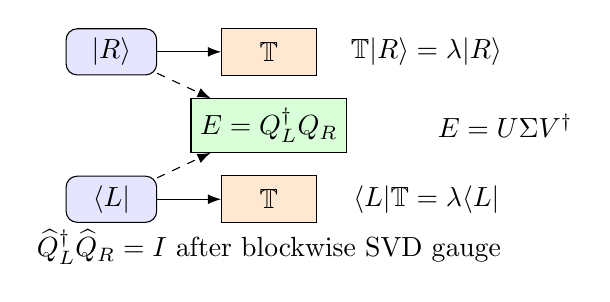
\begin{tikzpicture}[x=1cm,y=.72cm,>=Latex,
  m/.style={draw,rounded corners,fill=blue!10,minimum width=1.15cm,minimum height=.55cm},
  op/.style={draw,fill=orange!18,minimum width=1.2cm,minimum height=.6cm},
  g/.style={draw,fill=green!15,minimum width=1.35cm,minimum height=.6cm}]
  \node[m] (r) at (0,1.3) {$|R\rangle$};
  \node[op] (tr) at (2.0,1.3) {$\mathbb T$};
  \node[m] (l) at (0,-1.3) {$\langle L|$};
  \node[op] (tl) at (2.0,-1.3) {$\mathbb T$};
  \draw[->] (r)--(tr);\draw[->] (l)--(tl);
  \node at (4.0,1.3) {$\mathbb T|R\rangle=\lambda|R\rangle$};
  \node at (4.0,-1.3) {$\langle L|\mathbb T=\lambda\langle L|$};
  \node[g] (e) at (2.0,0) {$E=Q_L^\dagger Q_R$};
  \node at (5.0,0) {$E=U\Sigma V^\dagger$};
  \draw[->,dashed] (l)--(e);\draw[->,dashed] (r)--(e);
  \node at (2.0,-2.15) {$\widehat Q_L^\dagger\widehat Q_R=I$ after blockwise SVD gauge};
\end{tikzpicture}
\caption{标准非 Hermitian bi-VUMPS 的左右固定点和双正交 gauge。当前生产实现还没有执行这条独立左右 MPS 的 SVD gauge 流程。}
\label{fig:bi-vumps-flow}
\end{figure}

\section{技术总览：双边环境、方程与 bare 收缩}

这一节先给出实际代码所解的对象。这里的系统在空间方向是无限的；
$\chi$ 是边界 MPS 的 bond dimension，$D=2$ 是物理 PEPS 的虚键维度。
因此我们不先造一个有限的 $L\times L$ PEPS 再截断，而是直接在无限一维
transfer channel 上求上下两个边界 MPS 的固定点。有限的 $n$ 只出现在
数学上定义每格本征值的极限，不是数值计算使用的 window size。

\subsection{局域张量和双边环境}

固定物理 Fock 顺序后，一个 site 的 fermionic PEPS 张量写成
$A^p_{l r u d}$，其中 $p$ 是物理腿，$l,r,u,d$ 是有向虚腿；本例
$D=2$。把一行 PEPS 与其 bra 叠在一起得到一个有符号的 MPO 行 $O$。
上下边界是两条独立的无限 MPS：上边界记作 $R=(A_L,C,A_R)$，
下边界记作 $S=(B_L,D,B_R)$。$S$ 先取空间方向的 bra，并保留
fermionic graded leg 的方向和 parity；它不是把 $R$ 做一次未经验证的转置。

\begin{figure}[htbp]
\centering
\begin{tikzpicture}[x=1cm,y=0.72cm,>=Latex,
  mps/.style={draw,rounded corners,fill=blue!10,minimum width=1.05cm,minimum height=.52cm},
  peps/.style={draw,fill=orange!18,minimum width=.75cm,minimum height=.58cm},
  phys/.style={draw,fill=green!13,minimum width=.52cm,minimum height=.45cm}]
  \node[mps] (r1) at (0,1.55) {$R$};
  \node[mps] (r2) at (1.45,1.55) {$R$};
  \node[mps] (r3) at (2.9,1.55) {$R$};
  \draw[->] (-.75,1.55)--(r1.west); \draw[->] (r1.east)--(r2.west);
  \draw[->] (r2.east)--(r3.west); \draw[->] (r3.east)--(3.65,1.55);
  \node[peps] (a1) at (0,.35) {$O$};
  \node[peps] (a2) at (1.45,.35) {$O$};
  \node[peps] (a3) at (2.9,.35) {$O$};
  \node[phys] (p1) at (0,-.55) {$p$};\node[phys] (p2) at (1.45,-.55) {$p$};\node[phys] (p3) at (2.9,-.55) {$p$};
  \draw[->] (a1.south)--(p1.north);\draw[->] (a2.south)--(p2.north);\draw[->] (a3.south)--(p3.north);
  \draw[->] (-.75,.35)--(a1.west);\draw[->] (a1.east)--(a2.west);\draw[->] (a2.east)--(a3.west);\draw[->] (a3.east)--(3.65,.35);
  \node[mps] (s1) at (0,-1.65) {$S$};\node[mps] (s2) at (1.45,-1.65) {$S$};\node[mps] (s3) at (2.9,-1.65) {$S$};
  \draw[->] (-.75,-1.65)--(s1.west);\draw[->] (s1.east)--(s2.west);\draw[->] (s2.east)--(s3.west);\draw[->] (s3.east)--(3.65,-1.65);
  \draw[dashed] (-.8,2.15)--(3.7,2.15);\draw[dashed] (-.8,-2.15)--(3.7,-2.15);
  \node at (4.55,1.55) {上边界 $R$};\node at (4.55,.35) {PEPS 行 $O$};\node at (4.55,-1.65) {下边界 $S$};
\end{tikzpicture}
\caption{双边环境的实际对象。横向无限方向由箭头连接；纵向的 $O$ 是一整行
PEPS transfer MPO。每一个局部求解都重新使用当前的 $R,S$ 构造混合环境。}
\label{fig:bilateral-environment}
\end{figure}

\subsection{解的两个固定点方程}

将 PEPS 行夹在 $R,S$ 之间得到混合 transfer channel $\mathcal T_A$，
直接把上下边界相接得到重叠 channel $\mathcal T_0$：
\begin{equation}
  \mathcal T_A(R,S)=\mu_A R,\qquad
  \mathcal T_0(R,S)=\mu_0 R,
  \qquad q=\frac{\mu_A}{\mu_0}.
\end{equation}
实际实现不把这两个式子当成一个 Hermitian 本征问题；左右固定点、
混合度量和 fermionic parity 都保留。混合正交中心满足
$A_C=A_L C=C A_R$。对于上边界，代码分别检查
\begin{equation}
 H_{AC}^{(R)}(A_C)=z_{AC}^{(R)}N_{AC}^{(R)}(A_C),\qquad
 H_C^{(R)}(C)=z_C^{(R)}N_C^{(R)}(C),qquad
 z_{AC}^{(R)}=q_R z_C^{(R)};
\end{equation}
下边界 $S$ 另解同样的三式。最终的 \emph{joint residual} 是两侧的
AC/C 原始残差、去混合度量残差、$z_{AC}=qz_C$ 关系和两方向行商
不一致的最大值，而不是只看某个内层 cap 的残差。验收门槛是
$\epsilon_{\rm joint}<10^{-9}$。

\begin{figure}[htbp]
\centering
\begin{tikzpicture}[x=1cm,y=0.8cm,>=Latex,
  box/.style={draw,rounded corners,fill=blue!10,minimum width=1.0cm,minimum height=.55cm},
  op/.style={draw,fill=orange!18,minimum width=.9cm,minimum height=.65cm},
  arrow/.style={->,thick}]
  \node[box] (x) at (0,0) {$X$};
  \node[op] (o0) at (2,0) {$O_0$};
  \node[op] (oa) at (2,-1.45) {$O_A$};
  \node[box] (y0) at (4,0) {$\mathcal T_0(X)$};
  \node[box] (ya) at (4,-1.45) {$\mathcal T_A(X)$};
  \draw[arrow] (x)--node[above]{$R,S$}(o0);\draw[arrow] (o0)--(y0);
  \draw[arrow] (x.south)--++(0,-.55)-|node[pos=.25,below]{$R,S$}(oa);
  \draw[arrow] (oa)--(ya);
  \node at (6.0,0) {$\mu_0$ 主值};\node at (6.0,-1.45) {$\mu_A$ 主值};
  \draw[decorate,decoration={brace,amplitude=5pt}] (5.2,-1.72)--(5.2,.28)
    node[midway,right=7pt]{$q=\mu_A/\mu_0$};
\end{tikzpicture}
\caption{两种 transfer channel。$O_0$ 是上下边界直接重叠，$O_A$ 在中间夹一行
PEPS。$q$ 是每个横向 unit cell 的行商；数值上分别求左右主固定点，再检查两侧 joint 方程。}
\label{fig:two-channels}
\end{figure}

\subsection{外层优化与内层环境响应}

固定 $\chi$ 后，所有允许的边界参数组成向量 $a$。模型方向约束写为
$R=\mathrm{move}(a)$、$S=\mathrm{native}(a)$，但这只是参数化关系，
不是把 transfer matrix 假设为 Hermitian。每个 trial 参数都要重新解
cap 和左右环境；对 cap 方程 $M x=\mu x$ 的响应通过增广系统
\begin{equation}
 \begin{pmatrix}M-\mu I&-x\\x^\dagger&0\end{pmatrix}
 \begin{pmatrix}dx\\d\mu\end{pmatrix}
 =\begin{pmatrix}-(dM)x\\0\end{pmatrix}
\end{equation}
求出。外层以完整 residual 的解析 Jacobian $J$ 做信赖域最小二乘：
\begin{equation}
 \delta=\arg\min_{\|\delta\|\leq\Delta}\|F+J\delta\|^2,
 \qquad a_{\rm trial}=(a+Q\delta)(I+\delta^\dagger\delta)^{-1/2}.
\end{equation}
只有实际舍入候选的 merit gain 为正、独立有限差分通过、并且更新后的完整
joint residual 可计算时才接受；奇异方向不做截断。这里“内层收敛”指 cap/
响应线性问题收敛，“外层收敛”指双边 joint residual 过 $10^{-9}$，二者不等价。

\subsection{bare/direct 如何收缩三分区域}

环境通过后，三分区域的 $G$ 和 $B$ 不是另一个 VUMPS 近似：它们是固定边界
channel 的直接 leading fixed point：
\begin{equation}
 G=\operatorname{fp}\bigl(\text{top}\,|\,\text{bottom}\bigr),\quad
 B=\operatorname{fp}\bigl(\text{top}\,|\,A\,|\,\text{bottom}\bigr),\quad
 H_A=BG^{-1},\quad H_B=(G^{-1}\otimes I_{\rm phys})B.
\end{equation}
$G$ 是 two-column overlap，$B$ 是中间夹一个实际 PEPS tensor 的
three-column overlap；direct 方法不使用 grown tail 或 endpoint map。
三条区域边界由 $G,H_A,H_B$ 拼成带方向的 AB、AC、BC seams，
每个 seam 再用自己的 cap 做有限深度传播。replica 闭合时保留所有
fermionic parity sector 和有向指标，最后才做带符号的复数求和。

\begin{figure}[htbp]
\centering
\begin{tikzpicture}[x=1cm,y=.78cm,>=Latex,
  t/.style={draw,rounded corners,fill=blue!10,minimum width=.9cm,minimum height=.5cm},
  g/.style={draw,fill=purple!15,minimum width=1.0cm,minimum height=.62cm},
  h/.style={draw,fill=orange!18,minimum width=1.05cm,minimum height=.62cm},
  p/.style={draw,fill=green!15,minimum width=.62cm,minimum height=.62cm}]
  \node[t] (t1) at (0,1.35) {top};\node[t] (t2) at (1.45,1.35) {top};\node[t] (t3) at (2.9,1.35) {top};
  \node[t] (b1) at (0,-1.35) {bottom};\node[t] (b2) at (1.45,-1.35) {bottom};\node[t] (b3) at (2.9,-1.35) {bottom};
  \node[g] (g) at (1.45,0.28) {$G$};
  \node[h] (ha) at (0,0) {$H_A$};\node[h] (hb) at (2.9,0) {$H_B$};
  \node[p] (a) at (1.45,-0.48) {$A$};
  \draw[->] (t1)--(ha);\draw[->] (ha)--(b1);\draw[->] (t2)--(g);\draw[->] (g)--(a);\draw[->] (a)--(b2);\draw[->] (t3)--(hb);\draw[->] (hb)--(b3);
  \node at (1.45,-2.05) {$G=LR,\quad B=LTR$};
  \node at (1.45,2.05) {三列 bare 环境：无 grown tail、无 endmap};
\end{tikzpicture}
\caption{bare/direct 的局部收缩示意。中间的 $A$ 表示实际 PEPS tensor；
$G$ 与 $B$ 先由直接 leading fixed point 得到，再形成 $H_A,H_B$，而不是用优化后的 tail 替代。}
\label{fig:bare-direct}
\end{figure}

\subsection{fermionic replica 符号检查}

每条 seam 的传播保留 endpoint 的复相位和正范数 log scale；不能在每步把
复数投影成绝对值。$Z_2$ 的 character 表示只作浅层对照，$Z_4$ 的生产值使用
完整 signed cycle sum。检查顺序是：浅层 full/character 相对误差、每个深度的
复相位关系、endpoint residual、最后三档深度的长度漂移，最后才计算
$\tS=\log Z_{2A}+\log Z_{2B}+\log Z_{2C}-\log Z_4-2\log Z_1$。
因此一个漂亮的 $S$ 数字不能替代 joint 方程和符号门槛。

\subsection{当前双边求解算法：方程与迭代方法的区别}
\label{sec:current-pair-solver}

本节说明 2026 年 9 月 18 日的实验实现。可称为\textbf{固定 $\chi$ 的双边
VUMPS 驻点方程求解}；实际主算法是带模型方向约束的解析导数信赖域求根。
双正交投影负责生成初态，固定目标 $\chi$ 后重新优化，最后另做物理与熵验收。
逐条代码入口、作业号和可复制的 Slurm 提交命令见同目录
\href{two_sided_solver.md}{\texttt{two\_sided\_solver.md}}。

\paragraph{最新已完成结果与历史记录的区分。}
下文保留早期扫描与方法演变。当前$\chi=4,8,12$均通过原方向、实际旋转方向的
联合方程以及bare/direct收缩检查，熵分别为
$0.4903883073$、$0.6366027957$、$0.7652622556$。
另一个$\chi=6$、宇称扇区$(4,2)$驻点给出$0.5344557052$，
相关检查通过，但两点RDM误差稍大于$\chi=4$，不并入上述三点的斜率拟合。
$\chi=16$固定近似边界的$0.9114471196$仅为诊断熵：
长度与相位通过，环境残差约$5.29\times10^{-5}$，尚未通过。
这个熵只与同一分支的$\xi_{\rm MPS}=15.207702$、
$\xi_{\rm pair}=70.589325$、$\xi_{\rm physical}^{N/F}=71.161584$对应，
不能混用其它较小残差分支的关联长度。高精度续算中间记录不作为终态。
完整表格见Markdown开头，作业进度和复现命令见实验README。

\paragraph{新完成的原方向 $\chi=16$ 驻点。}
作业11343802在7个接受步后达到原始完整联合残差
$8.7391\times10^{-12}$。同一组保存的ComplexF64 canonical张量，
不重新正则化而用128位原方程复评，残差为$4.7825\times10^{-13}$。
该分支的$\xi_{\rm MPS}=5.9351838193$、$\xi_{\rm pair}=23.8104118804$，
normal/anomalous的$\xi_{\rm physical}=24.3359837271$，
connected density的$\xi_{nn}=4.9853374410$。
三档模权重阈值$10^{-10},10^{-8},10^{-6}$均稳定，64个距离的模重构误差
小于$10^{-13}$。这些长度略小于$\chi=12$；驻点收敛不证明物理精度随$\chi$
改善。Gaussian对照给出两点RDM最大误差$3.92050\times10^{-5}$，
略大于$\chi=12$的$3.63918\times10^{-5}$；积分网格漂移仅$6.16\times10^{-11}$。
在$r=31$处normal绝对误差为$1.81232\times10^{-4}$，anomalous与connected
density相对误差分别为$5.83454\%$、$41.3901\%$。
实际旋转模型求解尚待完成，没有新bare熵，
尤其不能配用上文旧分支的$0.9114471196$。

本次求解使用\path{benchmark/selected_precision_weighted_trust.jl}。
每轮从完整Float64响应矩阵开始，在软方向逐步以128位响应修正，
始终保留全部128个参数方向。实际步相对新算128位响应的误差须小于$10^{-8}$，
否则修正数从16增至32、64或全部；末步16和32均失败，64才通过。
原两档四阶差分、实际舍入候选的真实下降和完整联合残差门槛保持不变。
这不是截断小奇异值，也没有改变目标$\chi$。实际旋转模型采用自己的
PEPS和检查点，通过显式模型方向入口另行审计、求解。

\paragraph{$\chi=24$ 初态的例外。}
从新收敛$\chi=16$做双边长行和混合度量谱投影时，原切口检查未通过。
目标切口两侧本征值约为$-8.44\times10^{-9}$、$-3.77\times10^{-9}$；
局部相对间隔虽约为0.553，但相对$10^{-12}$的输入扰动使投影变化约
$0.12\%$--$0.45\%$，超过预设$10^{-3}$门槛。
纯对角相似变换平衡没有使原坐标下的相同扰动通过。
这是初态谱截断的稳定性问题，并非已经证明$\chi=24$优化失败。

另一个隔离初值将$\chi=16$按宇称等距嵌入$\chi=24$的$(12,12)$虚空间，
只在旧虚空间块外加$10^{-3}$扰动，然后规范化并重建上下关系。
\textbf{它不是双正交谱截断}；后续仍须在目标$\chi=24$参数空间求解原双边方程。
作业11345054保存初态的两侧每格fidelity均约为0.9999997254，
chart重建的fidelity误差小于$7\times10^{-14}$。
初始joint为0.0239161、$\xi_{\rm pair}=37.3894$；这些只是零步快照，
不是新收敛点，没有相应熵。较大的初始$\xi$也不证明物理精度改善。
高精度响应与完整Jacobian检查使用自己的初态和检查点，
入口控制仍与原$\chi=4$比较；命令见实验目录
\path{wide_model_precision_submissions.json}。原符号收缩和最终门槛不变。

\paragraph{实际旋转模型与大 $\chi$ 收缩的独立检查。}
实际旋转$\chi=16$的完整128位Jacobian和自适应精度求解，前12个接受步的
joint最大相对差为$1.30\times10^{-8}$，$\xi_{\rm pair}$最大绝对差为
$1.78\times10^{-9}$，但两者终点joint仍约$5.97\times10^{-6}$，未过门槛。
原方向通过不能代替实际旋转方向，也不能配用旧分支的熵。

旧未收敛$\chi=24$环境在bare深度4还显示最终闭合的数值敏感性：
冻结同一组四副本端点，仅换sliced边，单项复数结果最大相对差为
$3.44\times10^{-7}$。将已算出的标量项改用128位求和后，full/character
偏差仍约$5.68\times10^{-8}$，不能归因于最后标量累加。
随机复数graded网络的26项直接/优化/sliced对照通过，但不能保证这些病态
端点的精度。保持全部宇称和指标、逐项精确可逆的二进制成对缩放虽降低
范数包络，仍未改善两种闭合结果，未加入生产bare路线。
这些诊断使用旧未收敛环境，不能外推为新$\chi=24$或32收缩失败。

\paragraph{二副本传播误差的高精度定位。}
作业11346975在旧$\chi=24$、bare深度4的同一组Float64几何张量与cap上，
逐元素精确提升后重算传播、正范数归一化及最终张量闭合。
完整带符号表示与character表示的相对差在128/192位分别为
$2.07620\times10^{-31}$与$5.26863\times10^{-51}$；两档精度的
signed/character结果分别相差$7.89525\times10^{-32}$与$1.28715\times10^{-31}$。
signed结果相对原Float64改变$2.52973\times10^{-9}$。
只提升最后闭合精度时差异仍约$9.50\times10^{-10}$，因此这里定位到了
传播/归一化的浮点误差。没有改变符号、环境、$G/B$、cap或验收门槛。
这只验证二副本$Z_{2,C}$在深度4的数值；四副本高精度收缩尚未验证，
旧环境仍未收敛，没有新增熵点。来源与独立十进制复算见实验目录
\path{two_replica_propagation24_audit/local_verification.json}。

\paragraph{$\chi=24$求解准备检查。}
常规分区作业11346769完成全部288个参数方向的128位Jacobian/SVD，
没有截断奇异方向。重构误差$1.73\times10^{-37}$，实际方向误差
$1.04\times10^{-25}$，两档四阶差分误差$6.34\times10^{-8}$和$3.96\times10^{-9}$。
只读候选降低加权目标，但完整joint暂时增大，不能视为收敛点。
自己的自适应响应检查11346770已启动，后续求解仍需通过该检查。

\paragraph{调度终止与检查点恢复。}
\texttt{PREEMPTED}和\texttt{TIMEOUT}不是数值门槛失败。须先由
\texttt{sacct}确认终态，并由整个\texttt{squeue}确认父作业退出。
\path{restore_model_precise_checkpoint.jl}直接恢复八个canonical张量，
要求零改动并复现记录的joint与$\xi$；恢复报告标为\texttt{snapshot\_only}，
不是优化终态。续算使用原模型模板与恢复检查点，重新检查自己的响应和Jacobian。
近期恢复链显式指定\texttt{--partition=htc}以覆盖脚本默认的抢占分区，
精确命令见实验目录\path{regular_partition_recovery_submissions.json}。

\paragraph{双边方程。}
上下无限 MPS 记作 $R,S$，$\langle L|$ 由 $S$ 的空间边界 bra 构造，
包含原有腿方向、共轭和费米子 twist。定义每格行本征值商
\begin{equation}
 q(R,S)=\lim_{n\to\infty}
 \left[\frac{\langle L_n|T_n|R_n\rangle}
 {\langle L_n|R_n\rangle}\right]^{1/n}
 =\frac{\mu_T}{\mu_0}.
\end{equation}
这里 $\mu_T$ 是双方夹一行 PEPS 的水平混合通道主本征值，
$\mu_0$ 是双方直接重叠通道的主本征值。环长 $n$ 仅用于解释定义；
实际求无限通道固定点，没有构造有限环来代替环境。

每次从当前整对边界重新计算 $l_T,r_T,l_0,r_0$。
在混合正交形式 $A_C=A_LC=CA_R$ 下，两个方向分别要求
\begin{equation}
 H_{AC}(A_C)=z_{AC}N_{AC}(A_C),\qquad
 H_C(C)=z_CN_C(C),\qquad z_{AC}=qz_C.
\end{equation}
$H$ 包含 PEPS 行，$N$ 是上下重叠的混合度量；双方各自规范化并不使
混合度量自动等于单位阵。$AC$ 比 $C$ 多一个局部 PEPS 张量，故其本征值
之间有 $q$ 因子。固定 $\chi$ 时这些是投影驻点条件，不是完整态空间内
$TR-qR$ 必须严格消失。实现见
\path{benchmark/selfconsistent_pair_core.jl}。

\paragraph{当前使用的方向约束。}
方程验收两个方向，但主求解器并非独立优化两套任意复数张量。
它使用已对当前 $w=1$ 模型核查的上下方向关系，写为
\begin{equation}
 S=\mathrm{native}(a),\qquad R=\mathrm{move}(S),\qquad a^\dagger a=I.
\end{equation}
$a$ 位于固定中性物理支持的实数表示内；$\mathrm{move}$ 在已核查的
mode 基中实施 $u=W^\dagger$ 的 Fock 变换，其中
\begin{equation}
 W=\begin{pmatrix}0&1\\-1&0\end{pmatrix}.
\end{equation}
这不表示行 transfer 是 Hermitian，也不能推广为任意非厄米模型的假设。
旧 $\chi=8$ anchor 仅确定局域物理支持基，不限制目标 MPS 的虚键维度。
目标虚空间内允许的实数参数全部优化，但实数、中性支持、方向关系和
宇称空间仍是约束。约束梯度小不足以验收，必须重建双方并检查原始复数方程。
原方向与实际旋转模型也分别求解；上下方向关系不是未经证明的 $90^\circ$
环境变换。

\paragraph{解析响应与信赖域迭代。}
当前求 $f=\log q$ 的驻点。令 $Q$ 是 $a$ 的正交补，切向梯度为
$g=Q^\dagger\nabla_a f$。环境响应由每个 cap 的 $Mx=\mu x$ 隐式求导：
\begin{equation}
 \begin{pmatrix}M-\mu I&-x\\x^\dagger&0\end{pmatrix}
 \begin{pmatrix}dx\\d\mu\end{pmatrix}
 =\begin{pmatrix}-(dM)x\\0\end{pmatrix}.
\end{equation}
因此更新张量时 cap 也参与求导。包括规范约束曲率项后得到 Hessian $K$，
在信赖半径 $\Delta$ 内求
\begin{equation}
 \min_{\|\delta\|\leq\Delta}\|g+K\delta\|^2,\qquad
 a_{\rm trial}=(a+Q\delta)(I+\delta^\dagger\delta)^{-1/2}.
\end{equation}
重新求 trial cap 和梯度，以实际与预测的梯度范数平方下降比决定接受，
再检查完整联合残差。Hessian 谱不截断；解析导数另由实际标量 $\log q$
的自适应差分核查。该求根方法不保证 $q$、联合残差或 $\xi$ 每步单调，
也不是最大化 fidelity。内层 cap／响应问题收敛不能替代外层边界驻点收敛。
实现为 \path{benchmark/analytic_joint_hessian.jl} 和
\path{benchmark/analytic_dense_trust_adaptive.jl}。
旧的逐边广义本征更新保留在 \path{benchmark/solve_selfconsistent_pair.jl}。

\paragraph{接受范数的导数补充审计（9 月 18 日）。}
上述 $K$ 是标量 $f$ 的 polar-chart Hessian，不自动等于实际接受范数的
完整导数。令 $g_a=\nabla_a f$，实际残差及其响应为
\begin{equation}
 F=(I-aa^\dagger)g_a,\qquad
 dF=(I-aa^\dagger)dg_a-da(a^\dagger g_a)-a(da^\dagger g_a).
\end{equation}
对 $da=QV$，真实水平响应含 $-V(a^\dagger g_a)$，而标量 Hessian 使用
$-V\operatorname{sym}(a^\dagger g_a)$。在 $\chi=6$ 的停滞点，有限差分
确认两者不同；最后被拒绝的小步，旧预测为 $-6.95\times10^{-9}$，实际
导数为 $+4.18\times10^{-9}$，自适应 Richardson 核查误差约
$1.32\times10^{-15}$。该事实不否定原标量 Hessian 的对称性检查。

独立脚本 \path{benchmark/projected_merit_trust.jl} 因此对实际 $F$ 的矩形
Jacobian $J$ 求 $\min_{\|\delta\|\leq\Delta}\|F+J\delta\|^2$，保留全部奇异
方向和原完整联合验收。$\chi=4$ 控制达到 $1.20\times10^{-14}$，但
$\chi=6$ 仍停在 $1.34\times10^{-3}$；此修正没有单独解决后者，也不能
解释全部历史停滞。原算法保留；$\chi=16$ 从同一端点比较到第 40 步，原方法与修正方法的
联合残差分别为 $1.64046\times10^{-3}$ 和 $1.64839\times10^{-3}$，未见明显加速。
已通过独立联合方程验收的 $\chi=8,12$ 结果不因此自动失效。

另用完整实数 Stiefel 切空间（含 $QV$ 和 $aK$，$K$ 为实反对称矩阵）
及残差 $g_a-a\operatorname{sym}(a^\dagger g_a)$ 作独立小 $\chi$ 控制。
保留规范冗余并核查解析响应后，$\chi=4$ 达到 $1.20\times10^{-14}$，
但 $\chi=6$ 仍停在联合残差 $1.44\times10^{-3}$，不能据此宣称已解决停滞。

\paragraph{双正交投影只生成初态。}
上下边界各吸收实际一行 PEPS 后，以双方增长张量构造混合度量。
若有 $m$ 个简并主模，则保留完整孤立主空间，以
$\Tr(r_j\ell_i)=\delta_{ij}$ 归一，使用
\begin{equation}
 D_N=\frac1m\sum_i r_i\ell_i,\qquad
 D_{S,\mathrm{bra}}=\frac1m\sum_i\ell_i r_i.
\end{equation}
这些量不假设为正定厄米矩阵。保留的左右 Schur 子空间 $V,U$ 给出
$J=(U^\dagger V)^{-1}U^\dagger$、$JV=I$、斜投影 $P=VJ$。
检查条件数、投影恒等式和谱分离，不切开未分辨的简并或共轭本征对。
这不是声称 SVD 奇异值有复共轭配对。

当前初态路线先投影至 $2\chi_{\rm target}$，中间投影两个宇称扇区等额保留；
再用已核查的交换代数与奇虚规范等价性拆分两份 graded 副本。
拆分后的宇称多重度由分解得出；$4\to6$ 为 $(3,3)$，$4\to8$ 为 $(4,4)$。
配对按双方与父态 fidelity 的乘积选择。此后在目标 $\chi$ 重新求解全部
允许参数，父态不再固定。实现为 \path{benchmark/upward_block_seed.jl}。

\textbf{目前没有直接优化 $\xi_{\rm pair}$。}
截断的混合度量谱与求 $\xi_{\rm pair}$ 的 transfer 谱不同，算法不保证
该关联长度随 $\chi$ 单调，也不保证仅靠度量截断就保留所有慢模。

\paragraph{验收与当前状态。}
联合残差取双方 AC/C 原始及去度量残差、中心本征值关系、方向行商一致性
的最大值，门槛为 $10^{-9}$。另外检查 cap 残差、主模间隙、度量条件数和
逆作用。通过后仍须核对 Gaussian RDM、带复相位的关联函数与物理衰减模，
再用独立旋转环境做 bare/direct 的符号、相位及长度检查。
优化时吸收 PEPS 行不改变熵的定义：仍为两列 $G$、三列 $B$、$H=BG^{-1}$，
不采用 grown-tail 或 endmap。

中间 $\chi=6,8,12,16,24$ 已按统一主算法扫描，但五个初次端点均未通过
联合门槛。另由 $\chi=4$ 双边增长后精修的 $\chi=8$，job 11316040，得到
\begin{equation}
 \epsilon_{\rm joint}=5.2717177477\times10^{-10},\qquad
 \xi_{\rm pair}=10.8218030113.
\end{equation}
这是新的驻点记录，与旧 $\xi_{\rm pair}\simeq241.34$ 的 $\chi=8$ 点分开。
当前已核对源文件 SHA 与最终保存态残差。实际旋转环境续跑 job 11316154
也已通过联合门槛，残差 $4.89935\times10^{-10}$，
$\xi_{\rm pair}=10.8218030043$。原方向物理模式核查 job 11316153 完成，
normal/anomalous 衰减长度为 $11.3474822773$，density 为 $2.3482498890$，
对所测 residue cutoff 稳定；这不代替 Gaussian 精度比较。
最终态 Gaussian 测量完成：两点 RDM 最大元误差 $1.59502\times10^{-4}$；
$r=7$ 的 anomalous 相对误差约 $1.63\%$，理论为零的 normal 实测幅度
$1.26142\times10^{-3}$。小残差不单独证明物理分支正确。

后续 bare/direct job 11316162 已通过 signed 对照、相位、端点与长度检查，得到
\begin{equation}
 \widetilde S_{\chi=8}=0.6366027956792,\qquad
 \xi_{\rm MPS}=2.6764831294.
\end{equation}
长度漂移 $6.99\times10^{-11}$，最终相位误差 $1.14\times10^{-10}$，
端点残差 $1.86\times10^{-13}$。这是该有限 $\chi$ 联合边界的 bare 结果，
仍不代表无限 $\chi$ 的物理熵已认证。

$\chi=12$ 后续原方向／实际旋转方向联合残差分别达到
$7.88\times10^{-12}$、$7.96\times10^{-12}$，bare job 11316385 也通过。
当前该新分支为
\begin{center}
\begin{tabular}{rrrr}
\toprule
$\chi$ & $\xi_{\rm MPS}$ & $\xi_{\rm pair}$ & bare $\widetilde S$\\
\midrule
4 & 1.1708770101 & 4.2618928289 & 0.4903883073404\\
8 & 2.6764831294 & 10.8218030113 & 0.6366027956792\\
12 & 6.1002248428 & 25.4980754180 & 0.7652622555597\\
\bottomrule
\end{tabular}
\end{center}
$\chi=12$ 的 bare 长度漂移 $2.92\times10^{-10}$，最终相位误差
$1.23\times10^{-10}$，两点 RDM Gaussian 最大元误差 $3.64\times10^{-5}$。
normal/anomalous 物理衰减 $\xi=26.03172382$，density 为 $5.16526142$，
均对所测 residue cutoff 稳定。一般有限 $\chi$ MPS 不必保持 Wick 关系，
其偏差作为诊断记录，不能单独替代物理验收。

同一组熵对 $\ln\xi$ 的相邻割线如下：
\begin{center}
\begin{tabular}{lrr}
\toprule
关联长度定义 & $\chi:4\to8$ & $\chi:8\to12$\\
\midrule
单边 MPS & 0.17685 & 0.15617\\
双边 pair & 0.15691 & 0.15012\\
单粒子物理通道 & 0.16946 & 0.15495\\
密度物理通道 & 0.16960 & 0.16321\\
\bottomrule
\end{tabular}
\end{center}
Gaussian 既有每结点 $\ln L$ 系数约 $0.1550$--$0.1553$；三个小 $\chi$
点不足以认证渐近相等，不按斜率是否接近 Gaussian 选择关联长度定义。
\begin{figure}[htbp]
\centering
\includegraphics[width=\linewidth]{../../code2d/fpeps/data/direct_chi_curve/joint_bare_smallchi.pdf}
\caption{新联合分支的三个有限 $\chi$ bare 点与不同关联长度。线段仅连接
数据，不代表渐近拟合。联合残差与收缩检查通过，物理精度仍随 $\chi$ 核查。}
\end{figure}
从通过验收的 $\chi=12$ 生成的 $\chi=16$ 新初态，首段 60 步求解
（11316591）仍失败：末态联合残差 $0.12649$，梯度约 $8.36\times10^{-5}$，
混合度量条件数约 $1.42\times10^6$。它说明梯度下降不能替代完整方程
验收；该端点不用于 bare 熵测量。其他初态续算与中间 $\chi$ 试验另行保留。
\paragraph{直接优化完整 AC/C 残差的隔离试验（2026-09-18）。}
旧方法沿 $\chi=8$ 初态继续到累计 320 步，联合残差仍为
$2.03001\times10^{-4}$，$\xi_{\rm pair}=23.83058$。
新增方法在相同的模型方向约束参数空间中，优化双方 $X=AC,C$ 的残差
\begin{equation}
 f_X=\frac{N_X^{-1}(H_XX)/z_X-X}{\|X\|},\qquad
 z_X=\frac{\langle N_XX,H_XX\rangle}{\langle N_XX,N_XX\rangle},
\end{equation}
并加入 $z_{AC}=qz_C$ 与两侧行商一致性残差。
中心 $C=\sqrt{\rho}$ 取自通道正密度的正平方根，响应由
$C\,dC+dC\,C=d\rho$ 给出；$AC$、$AR$、全部 cap 及逆度量均参与求导。
完整 Jacobian 的信赖域步按真实残差下降接受，最终仍以原复数
\texttt{joint\_audit} 的 $10^{-9}$ 门槛验收。这是新的残差求解试验，
不能称作已经收敛的标准双边 VUMPS。

$\chi=4$ 的 $10^{-3}$ 切向扰动控制两步恢复到联合残差
$5.31\times10^{-11}$。$\chi=16$ 从旧方法第 200 步 checkpoint 出发，
40 步后联合残差降到 $5.80173\times10^{-5}$，
$\xi_{\rm pair}=23.89812$，尚未通过验收；没有新的 bare 熵值。
该端点的物理测量另行提交，不能沿用旧端点的 Gaussian 误差。
平衡奇偶扇区的 $\chi=6$ 新试验停于联合残差 $3.92\times10^{-4}$。

某些 $\chi=16$ 更新方向在过小差分步长下误差反而增加，较宽步长审计已经通过：相邻两档 Richardson 误差为
$1.75\times10^{-6}$ 和 $3.90\times10^{-6}$。另建隔离试验：当原线性一致性检查不通过时，必须有实际方向
连续两档 Richardson 检查同时支持组装 Jacobian 与直接方向响应，才允许
接受较大步长。它明确改变内部更新检查，不能宣称原检查通过；最终联合
残差、cap 唯一性和逆作用门槛均不改变。提交命令和源 SHA 见 Markdown note。

\paragraph{完整响应基与中心因子的数值精度核查。}
后续试验保留全部右奇异向量，在其正交基中重新计算解析响应。
$\chi=4$ 扰动控制通过；$\chi=16$ 的40步终态为
$\epsilon_{\rm joint}=5.93617\times10^{-7}$，
$\xi_{\rm MPS}=5.93485$，$\xi_{\rm pair}=23.82446$。
两点 RDM 的 Gaussian 最大元误差为 $3.92011\times10^{-5}$。
该端点尚未通过 $10^{-9}$ 联合门槛，原始 $AC/C$ 残差也未通过，
不能仅以逆度量放大为由认定收敛，没有新增 bare 熵点。

独立检查另一个已完成的 $\chi=16$ FD 端点，发现最小 Schmidt 值约
$4.11\times10^{-6}$。自密度 $\rho$ 的两种构造仅差
$2.26\times10^{-15}$，但先对角化 $\rho$ 再开方重建 $AR$ 时，
右等距误差为 $1.74\times10^{-7}$；直接采用 MPSKit 中心因子的 SVD
正因子后，该误差为 $5.21\times10^{-12}$。这是新残差 cache 的数值
精度问题，不能据此解释全部旧 VUMPS 失败。
隔离修正保留全部奇异值，以未平方的中心奇异值构造 Sylvester 响应，
并检查 $AR$ 等距误差小于 $10^{-9}$。$\chi=4$ 扰动控制通过，
$\chi=16$ 一般方向导数通过，但实际更新方向的两档差分审计未通过，
因此尚未启动该版本的 $\chi=16$ 求解。环境特征向量的迭代精修另行审计。
原联合方程和 bare 检查门槛、已有通过结果均不改变。

\paragraph{精修分支与驻点诊断（最新完成结果）。}
以通过导数审计的 $\chi=12$ 增长初态启动精修求解，原方向停在
$\epsilon_{\rm joint}=5.28538\times10^{-5}$、$\xi_{\rm pair}=70.58932$；
实际旋转模型独立求解停在 $5.28560\times10^{-5}$、$70.58610$。
两者均未通过。原方向 $\xi_{\rm MPS}=15.20770$，含 PEPS 柱的
normal/anomalous 物理衰减长度为 $71.16158$，connected density 为
$12.13482$。两点 RDM 的 Gaussian 最大元误差为 $1.37193\times10^{-4}$；
$r=31$ 的 anomalous 相对误差为 $0.2571\%$，connected density 为
$81.81\%$。不能仅凭较大的 $\xi$ 判定环境更准确，没有新增 bare 熵值。

令 $F$ 是完整 $AC/C$ 规范化残差向量，$J$ 为切空间 Jacobian。
该端点 $\|F\|=1.14304\times10^{-5}$、
$\|J^{\mathsf T}F\|=1.35391\times10^{-10}$，但原始对数行商的水平梯度范数
仍为 $0.05960768$，沿单位梯度方向的有限差分确认这一非零导数。
因此残差平方和优化的停滞不等于原始商驻点，也不等于环境收敛；
小 $\|J^{\mathsf T}F\|$ 本身不证明局部极小值。
完整物理空间中，$AC$ 残差在 rank-2 支撑之外的范数约为
$3.8\times10^{-14}$，远小于其总范数 $1.07\times10^{-5}$；
主要残差不是该物理支撑遗漏造成的。$\chi=4$ 控制的原始商梯度约为
$1.47\times10^{-10}$。后续从此 $\chi=16$ 端点重启原始商梯度路线，
并继续已通过缩步长导数审计的 $\chi=6$ 试验；联合方程、旋转方向和
bare 验收要求不改变。完整诊断和提交命令见 Markdown note 及计算日志。

以下保留早期结果和失败尝试作为历史记录，具体最新输出见上述 Markdown note。


\paragraph{未收敛环境上的 bare/direct 诊断（2026-09-18）。}
进一步对上述精修原方向及独立实际旋转环境做完整带符号 direct 收缩，
不使用 grown tail 或 endmap。深度 $d=256,512,1024$ 的诊断值分别为
$0.9115819898,0.9114477391,0.9114471255$。
最后一次相邻漂移为 $6.13674\times10^{-7}$，而最后三个深度中的最大
相邻漂移仍为 $1.34251\times10^{-4}$，未通过 $10^{-7}$ 长度门槛。
最终相位误差 $3.23965\times10^{-9}$ 通过 $10^{-8}$ 检查，端点残差为
$8.54686\times10^{-11}$。环境联合残差仍约 $5.3\times10^{-5}$。
因此 $0.9114471$ 仅为未收敛边界的有限深度诊断值，不能加入通过点或斜率拟合。
$d$ 是无限边界上的收缩深度，不是有限物理系统大小。
原目录新增诊断图，保留原通过点曲线。
此端点完整宇称扇区 $\xi_{\rm MPS}=15.20770$，$\xi_{\rm pair}=70.58932$，
normal/anomalous 物理衰减长度 $71.16158$；后端只取偶扇区的
$\xi_{\rm boundary,even}=7.61087$ 不可与完整 $\xi_{\rm MPS}$ 混用。
正式环境与熵验收要求不变，诊断入口及可复制提交命令见 Markdown note 与计算日志。


\paragraph{延长 direct 收缩到 $d=4096$。}
同一固定环境的 $d=2048,4096$ 诊断值分别为
$0.911447119770$、$0.911447119579$。
最后三档的最大相邻漂移为 $5.69980\times10^{-9}$，
最终相位误差 $8.76556\times10^{-9}$，端点残差 $1.40009\times10^{-10}$。
原生产长度、相位和端点检查现已通过；重叠深度与原扫描一致。
这只更新上述 $d=1024$ 时的收缩结论，环境联合残差仍约
$5.3\times10^{-5}$。因此 $0.9114471196$ 是该固定近似边界的稳定
bare/direct 诊断值，仍不可加入环境通过点或拟合。诊断图已同步更新。

进一步的隔离试验以直接中心因子 $C$ 对水平梯度残差加权：
$F=(I-aa^\dagger)g$，$R=FC^{-1}$，导数保留
$dR=dF\,C^{-1}+F\,d(C^{-1})$。所有 Schmidt 值保留，满秩时零点不变。
这只是优化范数的条件调整，不是按双边关联长度截断。
随机及实际方向的两档四阶差分在 $\chi=4,16$ 均通过，
$\chi=4$ 的扰动恢复控制达到联合残差 $4.53241\times10^{-11}$。
$\chi=16$ 新试验尚未完成，不能与上面的已测 direct 分支混配熵和关联长度。


\paragraph{完整响应基续算终态及 Gaussian 初态对照。}
加权20步终态之后再以完整响应基迭代40步，所有奇异方向保留，
实际接受步均通过在线导数和真实 merit 检查，但终态联合残差仍为
$5.14574\times10^{-4}$，$\xi_{\rm pair}=55.86733$，
加权梯度范数为 $0.00856833$，后段明显停滞。
原收敛图已加入这段续算；它没有新增 bare 熵，不能与前述
$0.9114471196$ 所属的精修分支混配。

对有限 $L=256$ Gaussian 拟合初态做零步快照及相同物理测量，得到
联合残差 $2.54497\times10^{-3}$，$\xi_{\rm pair}=76.58528$，
$\xi_{\rm MPS}=11.85895$，两点 RDM 最大元误差 $5.25981\times10^{-4}$。
同一初态经20步标量优化后，联合残差为 $6.16033\times10^{-2}$，
$\xi_{\rm pair}=18.70539$，$\xi_{\rm MPS}=4.99088$，
两点 RDM 误差降至 $5.33160\times10^{-5}$。
包含 PEPS 柱的 normal/anomalous 衰减长度分别为 $76.62000$ 与 $19.19661$。
局域误差改善并不意味着环境联合方程收敛；大的关联长度本身也不认证精度。
这两个端点都没有独立旋转求解和 bare 熵。
前后关联函数图及原始作业、提交命令见 Markdown note 和计算日志。
$\chi=6$ 加权试验也未通过，当前本路线通过联合方程、独立旋转与
bare 检查的有限 $\chi$ 点仍为 $4,8,12$。


\subsection{最新更新：χ16导数检查与χ6新驻点}
χ16从χ8扩维的AC/C端点继续5步weighted求解后，完整联合残差从
$5.93617\times10^{-7}$变为$1.57924\times10^{-6}$，
$\xi_{\rm pair}=23.80965$，仍未达到$10^{-9}$。
停止原因是导数检查，不能据此证明局部极小值。
缩小差分步长使原随机方向通过，但实际更新方向的组装与fresh响应相对差
$1.19723\times10^{-8}$仍超过$10^{-8}$，两档四阶差分要求也未通过。
依赖续算未启动并已取消。两点RDM的Gaussian误差为$3.92187\times10^{-5}$。
原目录的收敛图已补入这5步；$\widetilde S=0.9114471196$仍只属于前述
另一对固定近似边界，其收缩检查通过而环境检查未通过。

χ6新$(4\text{ even},2\text{ odd})$分支从已通过双边χ12投影得到初态，
在目标χ6独立优化后，原方向与实际旋转方向分别8步达到联合残差
$3.13511\times10^{-10}$与$3.13533\times10^{-10}$。
$\xi_{\rm MPS}=1.1779819574$、$\xi_{\rm pair}=3.7197912081$、
$\xi_{\rm physical}^{N/F}=4.2486792497$、$\xi_{nn}=1.5667834813$。
短程RDM物理检查通过，但两点RDM的Gaussian误差$9.37354\times10^{-4}$
稍大于χ4的$7.76806\times10^{-4}$，不能称为更准确的分支。
完整带符号bare/direct作业11342433已提交，尚无该新χ6的熵。
具体审计、作业和可复制提交命令保存在实验README的最新记录中。


随后作业11342433已完成：χ6上述分支的bare/direct结果为
$\widetilde S=0.5344557051926131$，长度漂移$2.55795\times10^{-12}$，
深度256的相位误差$7.24909\times10^{-12}$，端点残差$1.81161\times10^{-13}$，
完整带符号收缩通过。原生单边收敛标志不改写；本次双边joint另行检查并通过。
物理精度仍未认证。该点在χ16诊断图中以独立空心菱形展示，不并入原4/8/12分支的斜率拟合。


\subsection{128-bit精度检查与Gaussian续算}
χ16五步weighted终态的完整128-bit Jacobian实际方向检查通过：
组装/fresh相对差$1.74580\times10^{-22}$，两档四阶差分误差
$6.47619\times10^{-9}$与$4.04766\times10^{-10}$。
保留全部128个奇异方向，SVD重构误差$4.58\times10^{-38}$。
这支持此前该方向受到Float64精度限制，并不证明所有失败都由精度造成。
将最好χ16保存态的AL/AR/C/AC逐元素提升、保持波函数不变后，
完整joint从$5.93617488432\times10^{-7}$变为$5.93617485555\times10^{-7}$。
原始AC残差仍主导，环境尚未通过$10^{-9}$。
只读步长测试中全步与四分之一步使weighted merit变差，十六分之一步才改善；
精确导数仍不能消除非线性步长限制。

隔离高精度求解器逐步核查实际方向，保存前将候选转回ComplexF64，
再对实际舍入候选检查merit下降。最终完整joint门槛、边界格式和bare后端不变。
χ4扰动控制11343214通过后，χ16续算11343215才会启动；
其物理模及xi/RDM/Gaussian测量分别为依赖作业11343263/64。
这些任务尚不构成新的χ16熵结果，提交命令保存在实验README。

Gaussian有限环拟合追加500步后，loss从$1.27969178812\times10^{-7}$
降至$1.27368096194\times10^{-7}$，梯度仍为$4.22498\times10^{-7}$。
新态导入与符号检查通过；零步joint=$2.22958\times10^{-3}$，
$\xi_{\rm MPS}=11.8685951781$，$\xi_{\rm pair}=64.5167962663$。
$\xi_{\rm physical}^{N/F}=64.6014971278$对三个留数阈值稳定；
密度长度在$10^{-10}$阈值下为$11.7900971213$，
在$10^{-8}$与$10^{-6}$下为$4.0532066637$，有明显阈值依赖。
两点RDM的Gaussian误差由$5.25981\times10^{-4}$增至$5.70563\times10^{-4}$。
该分支没有bare熵，不与其它分支的熵混配。


\subsection{最新计算状态与可复现提交顺序（2026-09-18）}

\paragraph{旋转方向的 $\chi=16$ 续算。}
实际旋转 PEPS 必须独立求解，不能用原方向的环境代替。前一条 v3 续算在
20 个接受步后正常结束，完整联合残差由
$5.0476826714\times10^{-6}$降到$2.2150587419\times10^{-6}$，
$\xi_{\rm pair}=23.8250794145$。同一保存态的128位只读复核给出
$2.2150587412\times10^{-6}$，所以这不是 Float64 评估误差。
完整谱测量给出
$\xi_{\rm MPS}^{N}=5.9353250743$、
$\xi_{\rm MPS}^{S}=5.9353250743$、
$\xi_{\rm pair}=23.8250794145$；偶、奇两个宇称扇区都检查，
最大反向谱误差小于$8\times10^{-16}$。该边界仍未通过$10^{-9}$联合门槛，
这些长度不能和旧未收敛分支的$\widetilde S$配对。

从该保存态出发的 v4 续算使用完全相同的方程、128位响应修正、
实际有限差分和正 merit gain 检查，只把迭代上限从20提高到60。
当前已接受5步，联合残差为$1.6521817495\times10^{-6}$、
$\xi_{\rm pair}=23.8134212407$；仍不是熵验收点。

\paragraph{$\chi=24$ 的导数审计与求解失败。}
嵌入初态的完整128位 Jacobian 有288个参数方向，全部奇异值保留，
SVD重构误差为$1.73\times10^{-37}$。实际方向组装误差为
$1.04\times10^{-25}$，两档四阶差分误差为
$6.34\times10^{-8}$和$3.96\times10^{-9}$。自适应响应审计只把8个方向提升到128位，
相对于完整矩阵的更新作用误差为$2.23\times10^{-11}$，检查通过。
这些都是只读候选检查，不是优化终态。

随后原始20步求解从$\widetilde S$的零步初态
$\mathrm{joint}=0.0239161408$开始，接受到第3步时为
$0.0119709884$；下一次重建平衡中心因子时出现
`factor\_center` 求逆失败。该作业已确认是数值路径失败，
没有生成可接受的边界或熵。失败不是 replica 符号门槛，也不能说明$\chi=24$
方程没有解。已另建只改变初始 trust radius 的隔离脚本，
把$0.05\sqrt{\chi}$改为$0.0125\sqrt{\chi}$，其余方程、响应、
merit、符号和最终联合门槛完全不变。

\paragraph{另一条 $\chi=12\to16$ 初态支路。}
旧的 $\chi=12\to16$ 分支初态联合残差为
$5.2853820450\times10^{-5}$、$\xi_{\rm pair}=70.5893249470$。
它自己的两方向128位导数检查、完整128方向 Jacobian 和自适应响应审计均通过；
全步候选使加权范数变差，四分之一步和十六分之一步才改善，
因此仍须由信赖域优化器继续求解，不能把只读候选当作新终态。

\paragraph{提交接口。}
所有宽版求解器的参数顺序必须严格为
\begin{verbatim}
SOURCE OUTPUT FULL_J_AUDIT CHECKPOINT MAXITER INITIAL_NOISE
       CACHE_AUDIT SELECTED_RESPONSE_AUDIT MODEL
\end{verbatim}
例如，使用已通过审计的$\chi=24$初态时：
\begin{verbatim}
sbatch --clusters=htc --partition=htc --time=04:00:00 --mem=32G \\
  jobs/run_cpu.sh --compiled-modules=existing --pkgimages=existing \\
  benchmark/wide_model_selected_precision_smallradius.jl \\
  NATIVE_SEED OUTPUT FULL_J_AUDIT INITIAL_PAIR.jls 20 0 \\
  CACHE_AUDIT SELECTED_RESPONSE_AUDIT native
\end{verbatim}
把 audit 或 checkpoint 路径放到$\texttt{MAXITER}$位置会在进入数值前触发
参数解析错误；这类调度失败不应被记录为物理或 VUMPS 失败。

\paragraph{当前熵验收规则。}
只有原方向和实际旋转方向都满足完整联合残差$<10^{-9}$，保存态的
128位复核也通过，并且 bare/direct 的完整费米子 signed cycle、character 浅层审计、
相位、端点和长度门槛全部通过，才写入$\widetilde S$。bare 测量固定使用
$G=LR$、$B=LTR$、$H_A=BG^{-1}$和$H_B=(G^{-1}\otimes\text{physical})B$；
不使用 grown tail 或 endmap。有限$\chi$验收仍不等于无限$\chi$物理精度认证。


\subsection{固定目标 $\chi$ 的双边自洽求解：历史记录}

一次性从 $\chi=8$ 压缩到 $4,6$ 不能实现向大 $\chi$ 的自洽推广。
新增独立求解器在每个目标 $\chi$ 同时更新实际上下边界，重新求取混合
$T$ 通道与重叠通道的左右固定点，构造 $H_{AC},N_{AC},H_C,N_C$。
局部广义本征方程满足归一化关系
\begin{equation}
 z_{AC}=\lambda_{\rm row}z_C,
\end{equation}
因为 $AC$ 方程比 $C$ 方程多一个局部 PEPS 张量。
每次更新后重新计算整对环境，检查双方原始及去度量的驻点残差和本征值一致性；
内层本征向量残差或相邻两步 fidelity 不足以认证外层收敛。
新联合判据与原 self-Galerkin 判据分别保存，不覆盖原生收敛标志。

初步 $\chi=4$ 经 19 步达到联合残差 $7.10\times10^{-9}$，
$\xi_{\rm pair}=4.261892833$。$\chi=6,8$ 的单调残差更新暂时停滞，
尚未通过联合判据；另已提交阻尼交替更新和从已收敛 $\chi=4$ 向上扩维。
扩维后的旧边界仅是初态，每一级必须在目标 $\chi$ 重新自洽。
$\xi$ 仅作诊断，不作为越大越好的目标，不预设其单调性。
新解还需独立旋转方向边界、Gaussian 观测量对照和原 bare/direct 熵检查，
不能沿用旧熵，也不能仅凭驻点残差认定物理解正确。
后续 $\chi=6$ 经阻尼交替及独立 Jacobian 求根找到同一驻点，联合残差最低
$1.46\times10^{-11}$，$\xi_{\rm pair}=15.837189840$；但两点密度矩阵的
Hermiticity Frobenius 误差为 $4.81\times10^{-4}$，故物理验收失败，不作为可信熵点。
新 $\chi=4$ 两点 Gaussian 密度矩阵最大误差为 $7.77\times10^{-4}$，旧解约
$1.91\times10^{-3}$；完整 $\xi_{\rm MPS}=1.170877180$，
$\xi_{\rm pair}=4.261892833$，有权重的单粒子物理通道 $\xi=4.788325859$。
独立求解旋转方向后，原 bare/direct 得到 $\widetilde S=0.490388307343$，
最大最终相位误差约 $3.69\times10^{-9}$，长度及端点检查通过。
这是该有限 $\chi$ 联合边界的收缩结果，尚不代表无限 $\chi$ 熵已认证。
实数表示中的后续精修将原方向和实际旋转方向的联合残差分别降至
$1.32\times10^{-14}$ 与 $2.25\times10^{-14}$。
重新运行完整 bare 检查得到 $\widetilde S=0.4903883073405$，
depth $128$ 的相位误差为 $1.09\times10^{-14}$，端点残差为
$1.03\times10^{-15}$；与前次熵相差约 $3\times10^{-12}$。
对应完整 $\xi_{\rm MPS}=1.170877010$、$\xi_{\rm pair}=4.261892829$。

对实际行本征值商的变分梯度作求根，在 $\chi=8$ 找到联合残差
$9.04\times10^{-12}$ 的新驻点。其完整谱给出
$\xi_{\rm MPS}=2.840836649$、$\xi_{\rm pair}=241.3402590$。
一至三点密度矩阵的厄米性、归一化和正定性通过；两点 Gaussian
最大误差为 $1.35\times10^{-4}$，优于原生 $\chi=8$ 的 $3.41\times10^{-3}$。
但连通密度关联在 $r=31$ 为 $2.85\times10^{-4}$，Gaussian 仅为
$1.09\times10^{-7}$，出现明显错误的慢衰减尾部。
normal/anomalous 算符耦合的物理衰减长度为 $11.93884$，密度通道则为
$137.08620$。因此该点不能仅凭驻点收敛或大 $\xi_{\rm pair}$ 获得物理认证，
也未被加入可信熵曲线。
\begin{figure}[htbp]
\centering
\includegraphics[width=\linewidth]{../../code2d/fpeps/data/direct_chi_curve/joint_chi8_physical_checks.pdf}
\caption{$\chi=8$ 的独立物理核对。红色联合驻点的局域误差减小，
但远距离密度关联明显偏离 Gaussian。右图使用保留正负号的对称对数坐标，
奇、偶距离分别连线，避免把非物理的负连通关联隐藏在绝对值中。}
\end{figure}

另一个有限精度问题出现在双边同时作用一行 $T$ 后再截断的试验中。
$\chi=8$ 原始增长张量的混合通道具有双重主本征值，数值模间隙约
$10^{-15}$；正则化后出现约 $7\times10^{-8}$ 的劈裂。
此时单独选择一个主本征向量构造双边度量不可靠。
该发现仅适用于这项双边增长试验，不能直接归因到原有 VUMPS 的全部停滞。
零 Schmidt 支撑消除虽通过态保持检查，但双重主模仍存在，未解决这一问题。
算法、逐步残差与提交方式见
\path{data/selfconsistent_pair_20260917/README.md}。

交替单边增长的 Petrov 更新使用当前另一侧边界作为测试空间，每个目标
$\chi$ 单独迭代。$\chi=32$ 的联合残差先降至 $2.14\times10^{-4}$，随后失稳，
并因混合主模间隙小于 $10^{-8}$ 而停止；没有新的可信大 $\chi$ 熵。
保存的最低残差候选有 $\xi_{\rm MPS,N/S}=24.9270/25.5407$、
$\xi_{\rm pair}=59.6810$。两点 Gaussian 密度矩阵最大误差为
$1.53\times10^{-5}$，anomalous 关联在 $r=31$ 的相对误差为 $1.72\%$。
但连通密度同一距离为 $3.01\times10^{-7}$，Gaussian 为 $1.09\times10^{-7}$，
误差大于旧 $\chi=32$ 的结果。因此局域改善不能替代联合收敛和长程核对。

后续将新旧左正则张量输运到同一虚腿规范并对齐整站相位，分别测试
$\alpha=0.25,0.1$ 的阻尼，$\chi=32$ 均在续算后失稳；$\chi=8$ 也仅减慢漂移。
历史外推的修复版本在 $\chi=8,32$ 分别停滞于联合残差
$2.58518\times10^{-3}$、$2.99242\times10^{-4}$，未达到驻点。
初版外推的拒绝候选曾覆盖当前态，该版本终态已作废；修复版增加了保存态
与最后接受行的残差一致性检查，并重新通过规范和相位审计。
\begin{figure}[htbp]
\centering
\includegraphics[width=0.95\linewidth]{../../code2d/fpeps/data/direct_chi_curve/damped_petrov_iterations.pdf}
\caption{独立目标 $\chi$ 的阻尼对照，均未收敛。横轴为累计步长
$\sum\alpha$，不是物理时间；$\chi=32$ 的阻尼从未阻尼第 20 轮状态开始。}
\end{figure}

大 $\chi$ bare 前置矩阵的独立预检通过：$\chi=4$ 与原核心的四张量
$G,B,H_A,H_B$ 完全一致；$\chi=32$ 的完整 $G/B$ 谱维数为 $512/2048$，
行权重与联合方程相差 $2.93\times10^{-14}$，矩阵求逆误差为
$1.96\times10^{-12}$。此预检没有计算四副本熵，原 bare 核心未改动。

\paragraph{完整简并主空间的增长与截断。}
双边同时增长后的原 $\chi=8$ 案例有两个偶宇称主模。
对完整主空间按实际 graded 迹配对对偶化，构造
$D_N=m^{-1}\sum_i r_i l_i^{\rm dual}$、
$D_S=m^{-1}\sum_i l_i^{\rm dual}r_i$，其中 $m=2$。
主空间内基底变化不变性及独立复非酉虚腿规范协变检查通过。
先保留 $2\chi$ 再作宇称保持分块，可以获得两个实际维数为 $\chi$ 的分量。
在 $\chi=8$，两分量经显式 odd 虚腿规范和相位对齐后的局部张量差小于
$2.5\times10^{-12}$；各分量的单边偶固定点唯一。
这些是本次张量的数值检查，不能把所有费米子主模简并均当作可删除的副本。

完整迭代中，$\chi=4$ 在第 69 轮达到截断映射固定点，
$\xi_{\rm pair}=4.2910270389$，但联合 Galerkin 残差仍为
$1.38485\times10^{-4}$。$\chi=8$ 的联合残差先降到
$2.61741\times10^{-3}$，随后 $\xi$ 漂移到约 $1146$；
下一轮混合主模间隙约 $2.3\times10^{-12}$，未通过唯一性检查。
所以这项分块修正尚未解决外层不稳定。
截断映射固定点、VUMPS 驻点、物理关联函数和 bare 收缩需分别检验，
此处没有新增可信大 $\chi$ 熵。
历史加速用 5 步复现 $\chi=4$ 的截断固定点（映射残差 $1.35\times10^{-11}$），
但 $\chi=8$ 仍停滞于映射残差 $1.10\times10^{-2}$；三轮复非酉规范控制通过。
$\chi=4$ 的短条带物理性检查通过，两点 Gaussian 误差 $7.71\times10^{-4}$，
$\xi_{\rm MPS,N/S}=1.1738678953$。

\paragraph{不构造完整 Hessian 的驻点求解。}
另用有限差分 Hessian-vector product 与 Krylov 子空间求实际混合行权重的驻点。
梯度试探仅需 $H/N$ 缩并，完整联合验收仍保留原有度量求逆和 AC/C 检查。
两档差分一致性、Hessian 双线性对称性及标量方向导数分别核对。
$\chi=4$ 两步回到联合残差 $1.09\times10^{-10}$、
$\xi_{\rm pair}=4.26189284$；与完整 Hessian 的方向作用相差小于
$2.49\times10^{-7}$。
$\chi=32$ 自适应缩小差分扰动后完成一次更新，梯度约减半，但联合残差
从 $2.05\times10^{-4}$ 升至 $1.13\times10^{-3}$；
$\chi=12$ 续算也出现梯度降低而联合残差升至 $0.249$ 的情况，均未收敛。

$\chi=32$ 的方向约束初态有
$\xi_{\rm MPS,N/S}=25.5406644451$、$\xi_{\rm pair}=59.7531442910$。
其两点 Gaussian 密度矩阵误差为 $1.53733\times10^{-5}$，与约束前接近；
$r=31$ 连通密度为 $3.17576\times10^{-7}$，Gaussian 为
$1.09259\times10^{-7}$，比约束前稍差。这是更新前环境的独立诊断，
不能继承为后续候选的物理检查或 bare 熵认证。

\paragraph{弱方向上的差分精度与直接本征响应。}
扩大 Krylov 空间后，$\chi=12$ 某一步的预测线性残差约为
$1.86\times10^{-11}$，而沿所得方向重新计算为 $0.918$。
因此不能仅依据基向量差分检查或投影方程预测值认证 Newton 步。
独立旋转 $\chi=32$ 的五步试算也未收敛，联合残差约为 $0.122$。

新增直接响应方法，对实际 graded 通道 $Mx=\lambda x$ 解
\[
\begin{pmatrix}M-\lambda I&-x\\x^\dagger&0\end{pmatrix}
\begin{pmatrix}\delta x\\\delta\lambda\end{pmatrix}
=\begin{pmatrix}-(\delta M)x\\0\end{pmatrix}.
\]
$\delta M$ 由原有 transfer 的双线性项构造；有效张量的归一化导数和
canonical 回缩曲率项均保留。$\chi=4,12$ 的完整 Hessian 对称性误差为
$4.25\times10^{-15}$、$1.44\times10^{-13}$，作用线性误差约
$2.1\times10^{-15}$；与实际标量方向导数和多档有限差分的交叉核对通过。
使用该响应求根，$\chi=4$ 两步达到完整联合残差 $7.66\times10^{-11}$。
新的求解仍需通过原有联合、物理和熵判据；小 $\chi$ 控制不认证大 $\chi$。

完整 $G/B$ 预检接入 bare 副本流程的端到端回归也通过：
$\chi=4$ 的拟合结果为 $\tS=0.49038830734036765$，与原程序保存值相同；
深度 $128$ 的相位及端点误差分别为 $1.09\times10^{-14}$、
$1.03\times10^{-15}$。缓存使用前核对原始边界及张量内容，仍未新增可信大 $\chi$ 熵。

\paragraph{固定目标 $\chi$ 与最新稳定性检查。}
向大 $\chi$ 推广采用每个目标维度分别求解双边环境；早期由 $\chi=8$
压缩的实验仅作截断诊断。局域物理支撑基使用小 $\chi$ anchor 不限制虚键维度，
$\chi=32$ 已直接从原有 $\chi=32$ 环境启动。$\xi$ 是诊断输出，
不以最大化 $\xi$ 或强迫其随 $\chi$ 单调作为优化目标。
先前主要比较 $\chi=4$ 控制与 $\chi=32$ 压力测试，尚不足以检验逐步推广。
目前优先补齐 $\chi=6,8,12,16,24$，统一使用解析响应、完整通道梯度和
自适应标量导数检查的 trust-region 算法。各点从对应维度的已有环境重新求解，
并排队测量双方 $\xi_{\rm MPS}$、$\xi_{\rm pair}$ 与 Gaussian 关联函数。
这批独立求解尚不证明相邻 $\chi$ 的扩维会回到同一支，亦暂无新的可信熵点。
解析响应的 trust-region 小 $\chi=4$ 控制得到联合残差
$7.66\times10^{-11}$；$\chi=32$ 第四轮保存态的残差为
$5.56\times10^{-4}$、$\xi_{\rm pair}=55.9758$，下一轮触发
dense 与 Krylov 环境所算梯度的一致性检查，尚未收敛。
独立扰动两个方向的审计表明，被检查的 $\chi=4,12,32$ 点没有梯度相消：
两方向梯度范数之和等于总梯度范数，方向间相对差小于 $1.4\times10^{-9}$。
梯度下降仍不保证完整联合残差下降；所有这些大 $\chi$ 中间态都不认证为熵点。
最新作业、检查与提交命令持续记入
\path{data/selfconsistent_pair_20260917/README.md}。

\subsection{双边谱约束的双正交截断试验}

2026-09-17 的早期独立试验从单边 VUMPS 已收敛的 $\chi=8$ 四方向边界
向 $\chi=4,6$ 压缩；这不等于双边联合方程已收敛。
用实际双边 mixed transfer 的左右固定点构造 $D=rl$，逐宇称扇区取双正交子空间，
验证 $P_LP_R=I$，再作
\begin{equation}
 A_{\rm new}=(P_L\otimes I\otimes I)A P_R.
\end{equation}
$D$ 不是物理密度矩阵，不假定正定；投影保留完整复数符号。
除了按双边本征权重模截断，还枚举共同保留指标，以两个方向、偶/奇扇区
各前三个非平凡慢模的对数衰减率误差筛选。此为有限候选的谱匹配试验，
不是一般变分最优算法，也不强制 $\xi$ 随 $\chi$ 单调。
四方向不降维 fidelity per site 误差小于 $4\times10^{-15}$。

普通权重截断的 $\chi=4,6$ 分别有 $\xi_{\rm pair}=3.862941445,6.078274089$；
慢模筛选分别得到 $6.335896979,7.272040645$，来源为 $7.146827277$。
这些压缩态的原生残差仍为 $10^{-3}$--$10^{-2}$，不继承输入的 VUMPS 收敛标记。
所有新边界仍接原 bare 两列 $G$、三列 $B$ 和 $H=BG^{-1}$，长度、相位及符号检查不放宽。
较大的 $\xi_{\rm pair}$ 不能替代 Gaussian 密度矩阵与关联函数对照。

输入审计还发现，旧的独立旋转 south 虽单边收敛，与旋转 north 配对后却有
两个相反相位的主模，偶扇区模间隙仅 $1.04\times10^{-11}$。
重新独立求解旋转 south（原方向 north 仅作初态）后，原生残差为 $8.86\times10^{-13}$，
主模唯一，两个方向的源 $\xi_{\rm pair}$ 相差约 $5\times10^{-9}$。
此处没有使用未经证明的方向变换；原 bare 三输入不变。
完整提交命令、候选、物理对照和状态见
\path{data/paired_truncation_20260917/README.md}，
汇总表图见 \path{data/direct_chi_curve/paired_xi_truncation.*}。

\subsection{只保留总 parity 不等于能重建全部 seam}

设 $W$ 是从保留空间到原始 cut 的 isometry，$P_s$ 是 seam 需要的 parity/string operator。
安全的压缩是保存
\begin{equation}
 P_s^{\rm eff}=W^\dagger P_sW,\qquad
 \delta_s=\|(I-WW^\dagger)P_sW\|.\label{eq:string}
\end{equation}
若 $\delta_s\ne0$，则即使 $P_s^2=I$，也未必有 $(P_s^{\rm eff})^2=I$。
例如总体 ket+bra parity 可以是边界对称性，但单独 ket parity 并不必然守恒。
不能无证据地把一个 retained index 强行拆成独立 ket/ bra parity eigenlabels。
解决方式是保留相应 string MPO 与压缩矩阵元，
对所需 operator closure 扩充保留子空间，或直接联合压缩多副本环境。
非正交 endpoint maps 则须用对应 metric/dual maps 替代这里的 $W^\dagger$，并报告条件数。

这也是为何“先算 norm 的 $\chi$，再取 $\chi^{\otimes4}$”是一种近似策略，
不是对所有 replica defect 的严格保证。
必须同时检查 bulk boundary residual 和 defect observable 的 $\chi$ 收敛；
在临界态中，两者可能需要不同精度。

\subsection{固定点的 sector、振幅与相位}

对一个简单孤立主本征值，令 $\langle l|r\rangle=1$，则
\begin{equation}
 T^n|b\rangle\sim\lambda^n|r\rangle\langle l|b\rangle.
\end{equation}
应保留 $\lambda$ 与 $\langle l|b\rangle$ 的完整复数信息。
若按最大模值选了与物理 cap 正交的 sector，即使残差很小仍是错误的 endpoint。
有简并、负/复的同模长主值时应保留主子空间或做显式 finite-tail 极限，
不能总假定一个 unit-norm 固定点足够。

目前 \code{sixr\_closure.jl} 多处通过 \code{log(abs(z))} 形成观测量。
新 backend 应先输出每个 $Z_k$ 的 $(\log|Z_k|,\arg Z_k)$ 与归一化账本，
再检查最终比值相位是否符合目标的有限网络参考。
范数和 purity 必须为非负实数；cube 至少要先核对其完整相位，再判断采用的熵分支。
不能把负号、零值或显著虚部自动压成一个看起来平滑的实数熵。

\section{代码改动范围与两条可行实现路线}

建议新增独立 fermionic backend 与 metadata 类型，先不改变已验证的 RK/TFIM production 路径。
以下是读过的接口及需要补充的内容；没有在本次 note 工作中修改它们。
\begin{longtable}{p{0.43\textwidth}p{0.51\textwidth}}
\toprule
现有位置/操作 & fermionic 版本的要求\\\midrule\endhead
\code{core/state.jl}：\code{layer}、\code{double\_layer}
& $A^*$ 的端口/伴随约定；双层内部 swap；保存原始 ket/bra 融合字典。\\
\code{core/indices.jl}：普通 \code{Index} 标签
& 标签只能指定 connectivity；增加 parity、arrow、ordered ports、fusion map 和符号约定版本。\\
\code{vumps/src/quantum\_sixr.jl}：
\code{\_quantum\_transfer\_site}
& 目前显式循环计算 $A\bar A$，无手写式\eqref{eq:handdl}的 crossing 因子；
不能仅换入 fPEPS 数组。\\
同文件：\code{\_host\_array}、\code{\_quantum\_boundary\_array}、grown tensor
& typed contraction 已注意 dual twists，但转 dense 后要保留 graded fusion/basis map；
有 TensorKit 容器不代表后续普通 ITensor 计算已自动 fermionic。\\
\code{core/sixr\_closure.jl}：rail orientation、\code{m2\_split\_boundary}
& 区分存储换轴与实际端口交换；split 必须是保存的 fusion map 的逆。\\
同文件：\code{m2\_seam\_wiring}、\code{m2\_seam\_apply}
& 编译带符号的 sewing；核对源词、目标词和 far cap，而非只把索引设成相同。\\
\code{core/sixr.jl}：\code{SIXR\_RAILS}
& 保留现有拓扑表；另加四端口顺序、对偶方向、parity operator 与 sector 信息。\\
\code{m2\_close\_octahedron}、\code{m2\_relabel\_endpoint}
& 前者实现完整中心 swap/cap 网络；后者实现式\eqref{eq:reuse}的 $W$。\\
\code{m2\_endpoint}、五 sector 的 log 组合
& 保留 cap amplitude、主子空间和复相位，增加相位失败与零范数诊断。\\\bottomrule
\end{longtable}

\paragraph{路线 A：显式 swap + 现有普通数值 contraction。}
构造有序腿的数据类型和一套 swap 编译器，
把 crossing 吸收进 local double layer、seam tiles 和小中心网络后再转成普通 ITensors。
优点是每个号能与手写图对照，适合最初的精确验证。
约束是任何会改变逻辑端口顺序的新 contraction 路径都必须经编译器，不能绕开。

\paragraph{路线 B：端到端 graded tensor backend。}
从 $V=\mathbb C^{1|1}$ 到 VUMPS、LMPS、seam 和闭合，全程使用实现 fermionic braiding 的空间类型与有向 map。
这可减少手工维护的 swap，但仍需自己定义正确的 $P^{\rm occ}$ 与普通 trace。
具体库版本是否支持相应空间、转换是否保留它们，要在实施时核对本地依赖并用小 tensor 测试；
本 note 不把未查证的 API 当作可运行方案。
尤其“有 $\mathbb Z_2$ charge block”不等于“交换采用 fermionic braiding”：
bosonic $\mathbb Z_2$ 对称张量也有同样的 charge 分块。

\paragraph{独立参考：Gaussian Schur complement。}
直接从局域 Gaussian map 和虚键 covariance 投影得到 $\Gamma$，
与局域系数 fPEPS 的 covariance 和 replica 标量比较。
按 KSVC 的 covariance 约定，输出具有
$\Gamma_{\rm out}=A_G+B_G(D_G-\Gamma_{\rm in})^{-1}B_G^T$ 的形式；
换 Majorana/cup 约定会改变相应符号，必须用单键和两站点检查固定。
这是验证 fPEPS 的有力第三条路径，但不能代替对截断后 six-$R$ 网络的验证。

\section{实施阶段、通过条件及本次已做的检查}
\subsection{建议分阶段推进}

\begin{longtable}{p{0.10\textwidth}p{0.35\textwidth}p{0.46\textwidth}}
\toprule
阶段 & 产物 & 通过条件\\\midrule\endhead
0 & 本文约定、$A$ 表与线序基础操作
& CAR 矩阵、graded permutation composition、fusion/unfusion、ordinary trace 全部一致。\\
1 & $1\times2,2\times1,2\times2$ 显式 fPEPS oracle
& 从全局有序算符式独立求振幅；交换虚键方向并同步变换后状态相同；
Fock overlap/covariance 一致。不要只比范数。\\
2 & 同一有限态的五个 replica sectors
& 显式八/四/双层 contraction 与式\eqref{eq:occupation}、Gaussian 逐项一致；
同时检查未分区连续的排列转换、复数态、不同合法边界。\\
3 & 单副本双层与有限 boundary MPS
& 显式原始范数 vs 局域 $a$；无截断 boundary 收缩完全一致；
奇偶分块截断后协方差/局域观测量随 $\chi$ 收敛。\\
4 & 有限 LMPS seam/cap/中心
& 式\eqref{eq:finiteidentity}成立；换 contraction tree、端口规范后完整 $Z_k$ 不变；
这一步优先于无限固定点。\\
5 & cycle 分解、six-$R$ 与复用
& 式\eqref{eq:factor}的 operator action、式\eqref{eq:reuse}、cap 投影、
完整四副本与六端点 closure 均一致。\\
6 & 固定严格 $D=2$ 的无限环境扫描
& $\chi$、主 sector、far-tail 长度与各 $Z_k$ 独立收敛；再研究 $\tS$ 对 $\xi_\chi$ 的变化。\\\bottomrule
\end{longtable}

阶段 1--5 的小尺寸 double precision 绝对/相对目标可以从 $10^{-12}$ 开始，
但若 $Z$ 极小或 metric 病态，应改用相应尺度或高精度；不应强求不合理的相对误差。
\emph{没有}在本次完成阶段 1--6；它们是下一轮实现的明确验收标准。

\subsection{最有区分力的反例和控制组}

\begin{enumerate}
\item 真空积态与偶总宇称的 occupied product state：所有归一化 purity/cube 为 1，$\tS=0$。
      后者能发现 FSWAP 与普通 SWAP 的混淆，真空不能。
\item $(|00\rangle+\lambda|11\rangle)/\sqrt{1+|\lambda|^2}$ 分布在 $A,B$，$C$ 为积态。
      令 $p=(1+|\lambda|^4)/(1+|\lambda|^2)^2$，应有
      $\gamma_{2A}=\gamma_{2B}=p$、$\gamma_{2C}=1$、$\gamma_4=p^2$、$\tS=0$。
\item 四到六模随机复 Gaussian 态，包含 odd/ even 全局 parity 样本及非连续原始分区。
      先做正确 Fock 重排再比对，避免所有测试碰巧没有 crossing。
\item 对 all-even 的人工腿空间，应精确退化为现有 bosonic 六端点 closure。
      但这一控制组自身不能认证 fermionic 符号。
\item 改变局域 leg order、有向 bond convention、相邻交换分解和 contraction tree，
      同步变换全部张量/算符后标量不变。改变 spin structure 则可能改变物理态，不要求不变。
\item 独立缩放每个 endpoint 及 metric，核对式\eqref{eq:ratio}的模与相位抵消。
      这一测试不能检出所有共同漏号，必须结合原始有限网络比较。
\end{enumerate}

\subsection{本次真实验证记录与限制}

伴随 \code{check\_signs.py} 通过 Slurm job \code{11211749} 运行，
补充显式 SWAP 矩阵检查后由 \code{11211764} 重跑通过；结果存于 \code{checks.json}：
\begin{center}
\begin{tabular}{p{0.57\textwidth}p{0.36\textwidth}}\toprule
检查 & 结果\\\midrule
$Q$ 外代数展开 vs $32\times32$ CAR 矩阵 & 最大误差 $0$；16 个非零元\\
逆序符号 vs 相邻交换序列 & 384/384 通过\\
Fock 重排后的 covariance & 最大误差 $1.11\times10^{-16}$\\
四模 grouped occupation cube vs Gaussian determinant 幅值 & 误差 $5.55\times10^{-16}$\\
Gaussian glue 的 $g_X^2=-I$ 与 $g_Ag_B=-g_C$ & 精确成立\\
两套纯态 replica gauge 的字典 & 共轭 $r=(234)$ 成立\\\bottomrule
\end{tabular}
\end{center}
这些检查不包括完整 fPEPS patch、式\eqref{eq:handdl}、VUMPS、LMPS 或 six-$R$。
已有 Gaussian 程序的其他规模测试属于其原有证据，本次没有重新运行它们。

\section{后续物理问题：先把符号和有限环境误差分开}

建议第一组研究量是在固定严格 $D=2$ 临界 KSVC 张量上，扫描 $\chi$，
同时记录 boundary 残差、各 seam residual、各 parity sector 的谱、
$Z_1,Z_{2X},Z_4$ 的对数模/相位与 $\tS$。
关联长度应写明来自哪个 transfer channel：
\begin{equation}
 \xi=-\ell\big/\ln|\lambda_1/\lambda_0|.
\end{equation}
费米子 Green function 常涉及 odd/string channel，密度等 even observable 涉及不同 sector，
boundary MPS 自转移的 $\xi_\chi$ 也不必等于物理单粒子 $\xi$。
与 Gaussian 的 finite-size 或 mass regulator 对比时，要用同一几何、junction 数目和明确的 length 定义。
有限 $\chi$ 不能未经检验直接视为在原始 Hamiltonian 中加某个 mass。

若以后需要一族严格有限 $D$ 态，可从 Gaussian projector 参数形变出发，
逐点计算 covariance 并验证 parent Hamiltonian。
直接给现有 Hamiltonian 加任意质量项，通常不能据此保证 GS 仍由同一个 $D=2$ 局域结构精确表示。
这一步应在符号基准通过后开展；目前最有价值的基准正是一个固定且严格可知的态。

\bigskip
\noindent\textbf{需要下一轮真正求解的核心问题：}
在式\eqref{eq:occupation}的目标约定下，把完整有限 fermionic replica 网络缩到 LMPS cut 后，
其 crossing/string 信息是否能由现有六个 rank-four endpoint 的保留空间忠实承载？
本文给出了判断它的 operator、cap 和 finite-network 检查，也给出了不成立时的完整四副本备选。
因此无需预先赌一个普适的“六个 $R$ 外再乘一个负号”公式。

\begin{thebibliography}{9}
\bibitem{hand} 用户手写参考：\href{../../fPEPS_renyi_2.pdf}{\code{PEPS/fPEPS\_renyi\_2.pdf}}，
2 页；第 1 页为 projector、bond、swap convention，第 2 页为双层候选公式与多副本问题。
\bibitem{ksvc} C. V. Kraus, N. Schuch, F. Verstraete, J. I. Cirac,
\emph{Fermionic Projected Entangled Pair States}, Phys. Rev. A 81, 052338 (2010),
\href{https://arxiv.org/abs/0904.4667}{arXiv:0904.4667}。
本文核对了本地 \code{Gaussian/note/0904.4667v2.pdf} 的 Eq.~(4)、Gaussian example 和 Appendix A。
\bibitem{corboz} P. Corboz, R. Orús, B. Bauer, G. Vidal,
\emph{Simulation of strongly correlated fermions in two spatial dimensions with fermionic projected entangled-pair states},
Phys. Rev. B 81, 165104 (2010),
\href{https://arxiv.org/abs/0912.0646}{arXiv:0912.0646}，特别是 parity、swap 与 open-leg ordering 的规则。
\bibitem{methods} 当前 PEPS 方法：\href{../detailed.pdf}{\code{PEPS/notes/detailed.pdf}}，
源文件 \code{methods.tex}；six-$R$ 字典与实现位于 \code{code2d/lmps/core/}，
quantum bridge 位于 \code{code2d/lmps/vumps/src/quantum\_sixr.jl}。
\bibitem{gaussian} Gaussian 项目 note：
\href{../../../Gaussian/note_gaussian_en/main.pdf}{\code{Gaussian/note\_gaussian\_en/main.pdf}}；
核对代码为 \code{maj\_tools.py}、\code{cube\_bdg.py}、\code{cube\_bdg\_validate.py}、
\code{bigcube.py}、\code{run\_point.py}、\code{cirac2\_model.py}。
注意正文列出的普通 replica 与有向 Gaussian glue 的区别。
\end{thebibliography}
\end{document}
